\documentclass[11pt,letterpaper]{article}

\usepackage[spanish]{babel}
\usepackage[utf8]{inputenc}
\usepackage[T1]{fontenc}

\usepackage{amsmath,amssymb,amsthm,mathtools}
\usepackage{geometry}
\usepackage{enumitem}
\usepackage{tikz}
\usepackage{pgfplots}
\usepackage{xcolor}
\usepackage{hyperref}
\usepackage{graphicx}
\graphicspath{{figuras/}}
\usepackage{float}
\usepackage{booktabs}
\usepackage{tcolorbox}
\tcbuselibrary{theorems,skins}
\pgfplotsset{compat=1.18}
\usetikzlibrary{arrows.meta,calc,positioning,babel}

\geometry{margin=2.4cm}
\setlength{\parindent}{0pt}
\setlength{\parskip}{6pt}
\hypersetup{colorlinks=true, linkcolor=blue, urlcolor=blue}

% ── Colores ────────────────────────────────────────────────────────────────
\definecolor{azul}{RGB}{37,99,235}
\definecolor{rojo}{RGB}{220,38,38}
\definecolor{verde}{RGB}{22,163,74}
\definecolor{gris}{RGB}{71,85,105}
\definecolor{fondodef}{RGB}{239,246,255}
\definecolor{fondoteo}{RGB}{240,253,244}
\definecolor{fondoobs}{RGB}{255,251,235}

% ── Entornos ───────────────────────────────────────────────────────────────
\newtcbtheorem[number within=section]{definicion}{Definición}{
  colback=fondodef, colframe=azul, fonttitle=\bfseries,
  separator sign none, description delimiters parenthesis,
  label type=definition}{def}

\newtcbtheorem[number within=section]{teorema}{Teorema}{
  colback=fondoteo, colframe=verde, fonttitle=\bfseries,
  separator sign none, description delimiters parenthesis,
  label type=theorem}{teo}

\newtcbtheorem[number within=section]{observacion}{Observación}{
  colback=fondoobs, colframe=orange!80!black, fonttitle=\bfseries,
  separator sign none}{obs}

\newtheorem{ejemplo}{Ejemplo}[section]

\newcommand{\dd}{\,d}
\newcommand{\cte}{\operatorname{cte}}
\newcommand{\naglecite}[1]{\emph{(véase Nagle, #1)}}

% ──────────────────────────────────────────────────────────────────────────
\title{\textbf{Apuntes de Modelos Matemáticos I}\\[4pt]
       \large Notas de clase y complementos con Nagle, Saff \& Snider (7a ed.)}
\author{Compilación y edición}
\date{Mayo--Junio de 2026}
% ──────────────────────────────────────────────────────────────────────────

\begin{document}
\maketitle

\tableofcontents
\newpage

% ============================================================
\section{Modelos elementales y origen de las EDOs}
% ============================================================

Los modelos matemáticos en fenómenos físicos pueden originarse a partir de:
\begin{itemize}
    \item \textbf{Leyes fundamentales} (Newton, conservación de energía, etc.),
          que son principios de validez general.
    \item \textbf{Leyes constitutivas} de carácter experimental, que capturan el
          comportamiento observado de un sistema específico.
\end{itemize}

\subsection{Caída libre}

La caída libre se modela mediante la Segunda Ley de Newton: $F=ma$. Si solo
actúa la gravedad, la aceleración es constante e igual a $g$, lo que conduce
directamente a una EDO de segundo orden. Cuando se añade resistencia del aire,
el problema se enriquece y aparece la noción de velocidad terminal; este caso
se estudia con detalle en la sección de adimensionalización
(§\ref{sec:adimensionalizacion}).

\subsection{Decaimiento radiactivo}

Sea $Q(t)$ la cantidad de elemento radiactivo al tiempo $t$. La \emph{pérdida}
de material en $[t,t+h]$ es proporcional a la cantidad presente:
\[
0\leq Q(t)-Q(t+h)\simeq kQ(t)h,\qquad k>0.
\]
Tomando el límite $h\to 0$:
\[
\boxed{\frac{dQ}{dt}=-kQ,\qquad k>0.}
\]
Como $Q(t)\geq 0$ y $k>0$, la función $Q(t)$ es monótona decreciente, lo que es
coherente con el hecho de que el material se desintegra con el tiempo sin regenerarse.

% ============================================================
\section{Separación de variables y solución analítica}
% ============================================================

El método de \textbf{separación de variables} \naglecite{§2.2} permite resolver
ecuaciones de la forma $y'=g(x)h(y)$ reescribiéndolas como
\[
\frac{dy}{h(y)}=g(x)\dd x
\]
e integrando ambos lados. La condición para aplicarlo es precisamente que el
lado derecho sea un producto de una función solo de $x$ por una función solo de $y$.

\subsection{Solución del decaimiento radiactivo}

Partimos del PVI $Q'=-kQ$, $Q(0)=Q_0$, $k>0$. La ecuación es separable porque
el lado derecho es $(-k)\cdot Q$, un producto de una constante (función de $t$)
por $Q$ (función de $Q$). Separando:
\[
\frac{1}{Q}\dd Q=-k\dd t
\;\Longrightarrow\;
\ln|Q|=-kt+C
\;\Longrightarrow\;
\boxed{Q(t)=Q_0e^{-kt}.}
\]
Como $k>0$, $\lim_{t\to\infty}Q(t)=0$: toda la sustancia se desintegra eventualmente.

\begin{figure}[H]
\centering
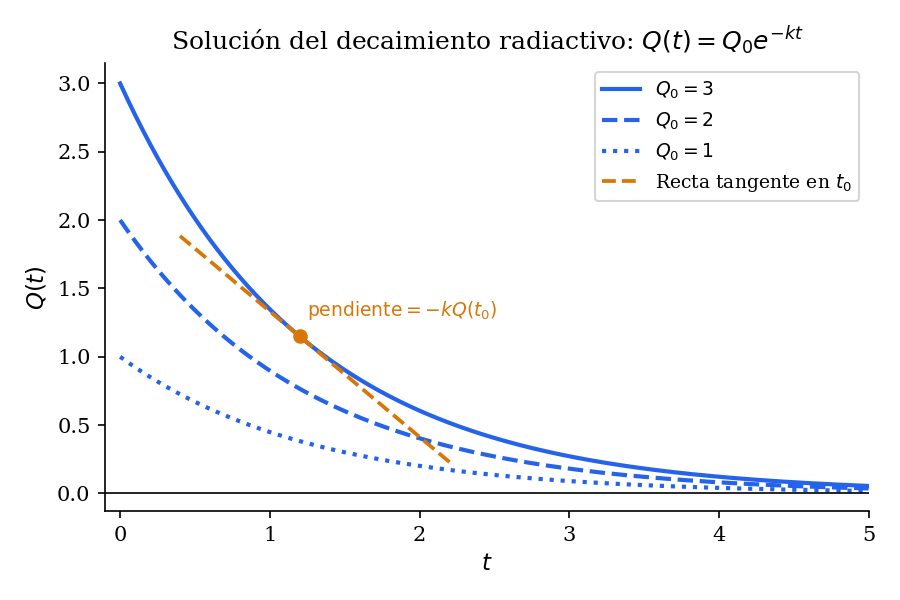
\includegraphics[width=0.72\textwidth]{fig_01_decaimiento_solucion.png}
\caption{Solución $Q(t)=Q_0e^{-kt}$ para distintos valores de $Q_0$. Todas las curvas
         son exponenciales decrecientes que convergen a cero.}
\end{figure}

\subsection{Vida media}

\begin{definicion}{Vida media}{}
La \textbf{vida media} $t_{1/2}$ es el tiempo necesario para que la cantidad inicial
se reduzca exactamente a la mitad: $Q(t_{1/2})=Q_0/2$.
\end{definicion}

De $Q_0e^{-kt_{1/2}}=Q_0/2$ se obtiene
\[
\boxed{t_{1/2}=\frac{\ln 2}{k}.}
\]

\begin{observacion}{Independencia de $Q_0$}{}
La vida media $t_{1/2}$ no depende de la cantidad inicial $Q_0$. Esto es consecuencia
directa de la estructura exponencial de la solución: si en $t=0$ hay el doble de material,
en $t=t_{1/2}$ también habrá el doble, y la proporción reducida es siempre la mitad.
\end{observacion}

\begin{figure}[H]
\centering
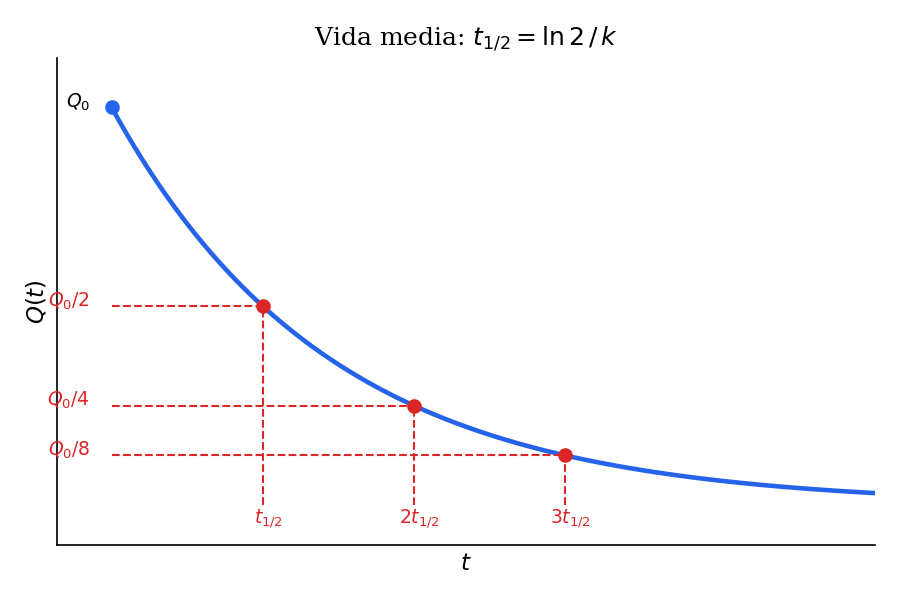
\includegraphics[width=0.72\textwidth]{fig_02_vida_media.png}
\caption{La cantidad se reduce a la mitad en cada intervalo de longitud $t_{1/2}$,
         independientemente del valor inicial.}
\end{figure}

% ============================================================
\section{Ecuaciones lineales de primer orden}
\label{sec:ecuaciones-lineales-primer-orden}
% ============================================================

Una ecuación de la forma
\[
\frac{dQ}{dt}+p(t)Q=g(t)
\]
se llama \textbf{lineal de primer orden} y se resuelve mediante el
\textbf{factor integrante} $\mu(t)=e^{\int p(t)\dd t}$ \naglecite{§2.3}.
La idea es que al multiplicar ambos lados por $\mu$, el lado izquierdo se
convierte en la derivada de un producto:
\[
\frac{d}{dt}\!\bigl[\mu(t)Q(t)\bigr]=\mu(t)g(t).
\]
Integrando ambos lados se obtiene la solución general. Esta técnica unifica
todos los problemas lineales de primer orden en un procedimiento sistemático.

\subsection{Modelo compartimental con entrada constante}

El caso más sencillo añade al decaimiento una \emph{entrada} constante $I>0$,
modelando por ejemplo la entrada de un fármaco al torrente sanguíneo:
\[
\boxed{\frac{dQ}{dt}=-kQ+I,\qquad I>0,\quad k>0.}
\]

\textbf{Punto de equilibrio:} cuando $Q'=0$ se obtiene $Q^*=I/k$, que es
asintóticamente estable: sin importar la condición inicial, el sistema tiende a
este nivel de saturación.

\textbf{Solución analítica} (con factor integrante $e^{kt}$):
\[
\boxed{Q(t)=\frac{I}{k}+\!\left(Q_0-\frac{I}{k}\right)e^{-kt}.}
\]
El primer término es el equilibrio; el segundo es un transitorio exponencial que
desaparece con el tiempo. Para cualquier $Q_0$: $\lim_{t\to\infty}Q(t)=I/k$.

\begin{figure}[H]
\centering
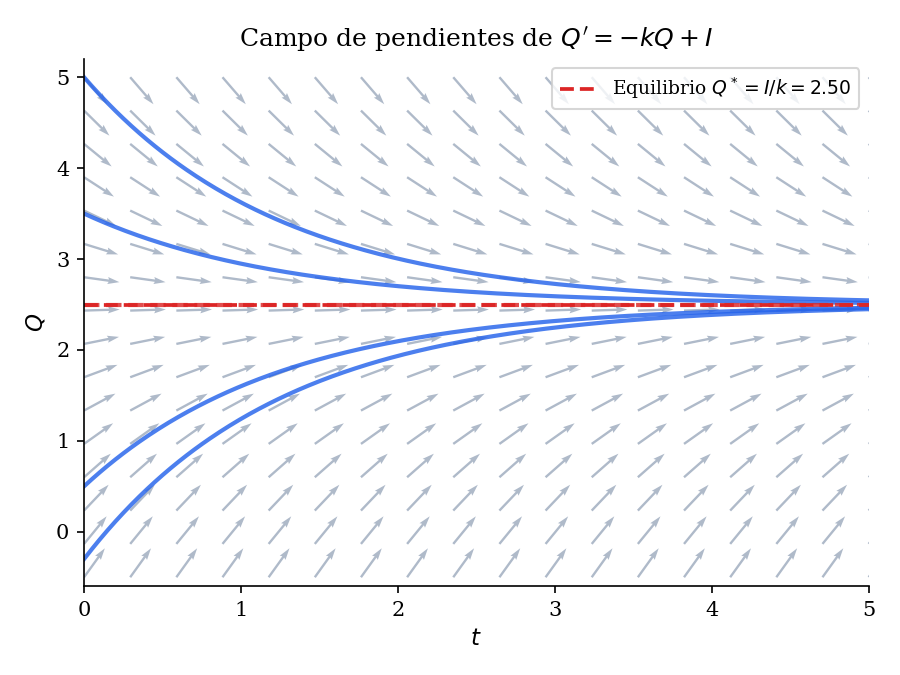
\includegraphics[width=0.74\textwidth]{fig_05_campo_compartimental.png}
\caption{Campo de pendientes de $Q'=-kQ+I$. Todas las trayectorias convergen a
$Q^*=I/k$, independientemente de la condición inicial.}
\end{figure}

\subsection{Circuito RC}
\label{sec:circuito-rc}

Un circuito RC con resistencia $R$, capacitor $C$ y voltaje constante $V_0$
satisface \naglecite{§3.5}, por la ley de Kirchhoff:
\[
R\frac{dq}{dt}+\frac{1}{C}q=V_0,
\]
donde $q(t)$ es la carga en el capacitor. Reescribiendo en forma estándar:
\[
\frac{dq}{dt}+\frac{1}{RC}q=\frac{V_0}{R}.
\]
Esta es una ecuación lineal de primer orden con $p=1/(RC)$ y $g=V_0/R$.
Con condición inicial $q(0)=q_0$, la solución es
\[
\boxed{q(t)=CV_0+\bigl(q_0-CV_0\bigr)e^{-t/(RC)}.}
\]
El equilibrio $q^*=CV_0$ es asintóticamente estable con constante de tiempo $\tau_c=RC$.

\textbf{Adimensionalización:} introduciendo
\[
\hat{q}=\frac{q}{CV_0},\qquad \hat{t}=\frac{t}{RC},
\]
la ecuación se reduce a la forma universal
\[
\frac{d\hat{q}}{d\hat{t}}=1-\hat{q},
\]
que tiene un único equilibrio adimensional $\hat{q}^*=1$ y describe la
dinámica del circuito sin depender de los valores particulares de $R$, $C$ ni $V_0$.
Esta forma es idéntica a la de la caída libre con resistencia, lo que pone en
evidencia la universalidad de la estructura matemática subyacente.

% ============================================================
\section{Cinética química}
\label{sec:cinetica}
% ============================================================

\subsection{Reacción elemental \texorpdfstring{$A\to B$}{A to B} (primer orden)}

Para la reacción $A\xrightarrow{k}B$ con condiciones iniciales $A(0)=A_0$, $B(0)=0$,
cada molécula de $A$ que se consume produce una de $B$, de modo que el sistema es:
\[
\boxed{\begin{aligned}
\frac{dA}{dt}&=-kA,\\[4pt]
\frac{dB}{dt}&=kA.
\end{aligned}}
\]

\textbf{Conservación de masa:} sumando las dos ecuaciones se obtiene
$\frac{d}{dt}(A+B)=0$, lo que implica que la cantidad total de material se conserva:
\[
\boxed{A(t)+B(t)=A_0,\qquad t\geq 0.}
\]

\textbf{Solución analítica:} La ecuación de $A$ es lineal homogénea y se resuelve
por separación de variables. Una vez obtenida $A(t)$, $B(t)$ se deduce de la conservación:
\[
A(t)=A_0e^{-kt},\qquad
B(t)=A_0\!\left(1-e^{-kt}\right).
\]

\begin{figure}[H]
\centering
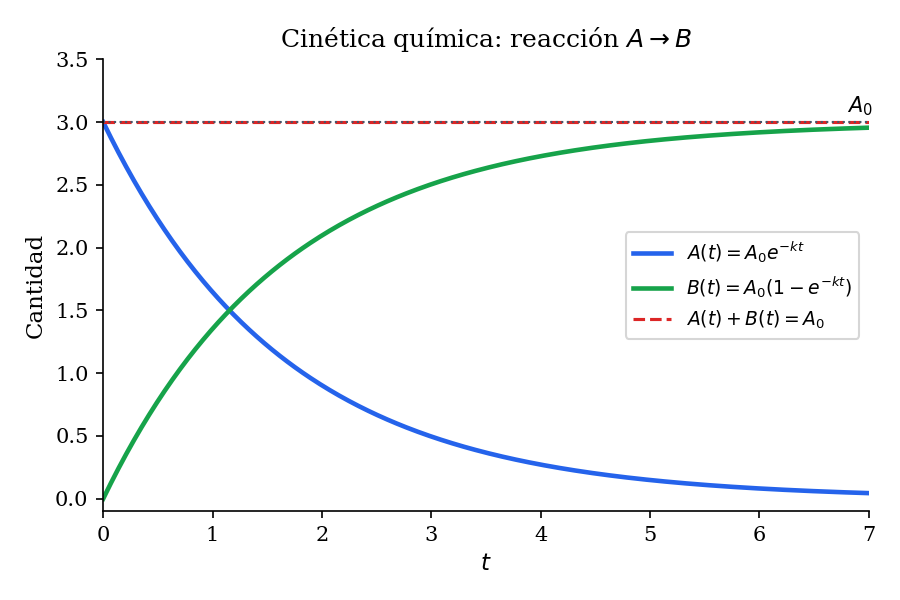
\includegraphics[width=0.72\textwidth]{fig_06_cinetica_AB.png}
\caption{$A(t)$ decrece exponencialmente; $B(t)$ crece de forma complementaria.
La suma $A+B=A_0$ (línea roja) se conserva para todo $t$.}
\end{figure}

\subsection{Ley de acción de masas}

\begin{definicion}{Ley de acción de masas}{}
Para la reacción $\alpha A+\beta B\xrightarrow{k}\cdots$, la velocidad de
reacción es proporcional al producto de las concentraciones elevadas a sus
coeficientes estequiométricos:
\[
v=kA^{\alpha}B^{\beta}.
\]
\end{definicion}

\begin{ejemplo}
\textbf{Reacción $2A\xrightarrow{k}B$.} Por la ley de acción de masas, $v=kA^2$.
Cada evento de reacción consume 2 unidades de $A$ y produce 1 de $B$:
\[
\frac{dA}{dt}=-2kA^2,\qquad \frac{dB}{dt}=kA^2,\qquad A(0)=A_0,\quad B(0)=0.
\]

\textbf{Conservación estequiométrica:}
\[
\frac{d}{dt}(A+2B)=-2kA^2+2kA^2=0
\;\Longrightarrow\;
\boxed{A(t)+2B(t)=A_0.}
\]

\textbf{Solución de $A$:} la ecuación $A'=-2kA^2$ es separable:
\[
\frac{dA}{A^2}=-2k\dd t
\;\Longrightarrow\;
-\frac{1}{A}=-2kt+C.
\]
Con $A(0)=A_0$: $C=-1/A_0$, de modo que
\[
\boxed{A(t)=\frac{A_0}{1+2kA_0 t}.}
\]
A diferencia de la reacción de primer orden, aquí la extinción de $A$ es algebraica
(hiperbólica), no exponencial: el proceso es más lento al disminuir la concentración.

\textbf{Solución de $B$:} usando la conservación,
\[
\boxed{B(t)=\frac{A_0}{2}\cdot\frac{2kA_0 t}{1+2kA_0 t}.}
\]
Nótese que $A(t)\to 0$ y $B(t)\to A_0/2$ cuando $t\to\infty$,
verificando $A_0+2\cdot 0=A_0$.
\end{ejemplo}

% ============================================================
\section{Modelos poblacionales}
% ============================================================

\subsection{Modelo malthusiano \naglecite{§3.2}}

Bajo hipótesis de tasas de crecimiento y mortalidad constantes, sin interacciones
ni limitación de recursos, la variación de la población en cada instante es
proporcional al tamaño actual:
\[
\boxed{\frac{dN}{dt}=rN,\qquad r\in\mathbb{R}.}
\]
La solución es $N(t)=N_0e^{rt}$, y el comportamiento depende cualitativamente del
signo de $r$:
\begin{itemize}
    \item $r>0$: crecimiento exponencial ($N\to+\infty$); irrealista a largo plazo.
    \item $r<0$: extinción ($N\to 0$); aplicable a poblaciones en declive.
    \item $r=0$: población constante; poco frecuente en la naturaleza.
\end{itemize}

\begin{figure}[H]
\centering
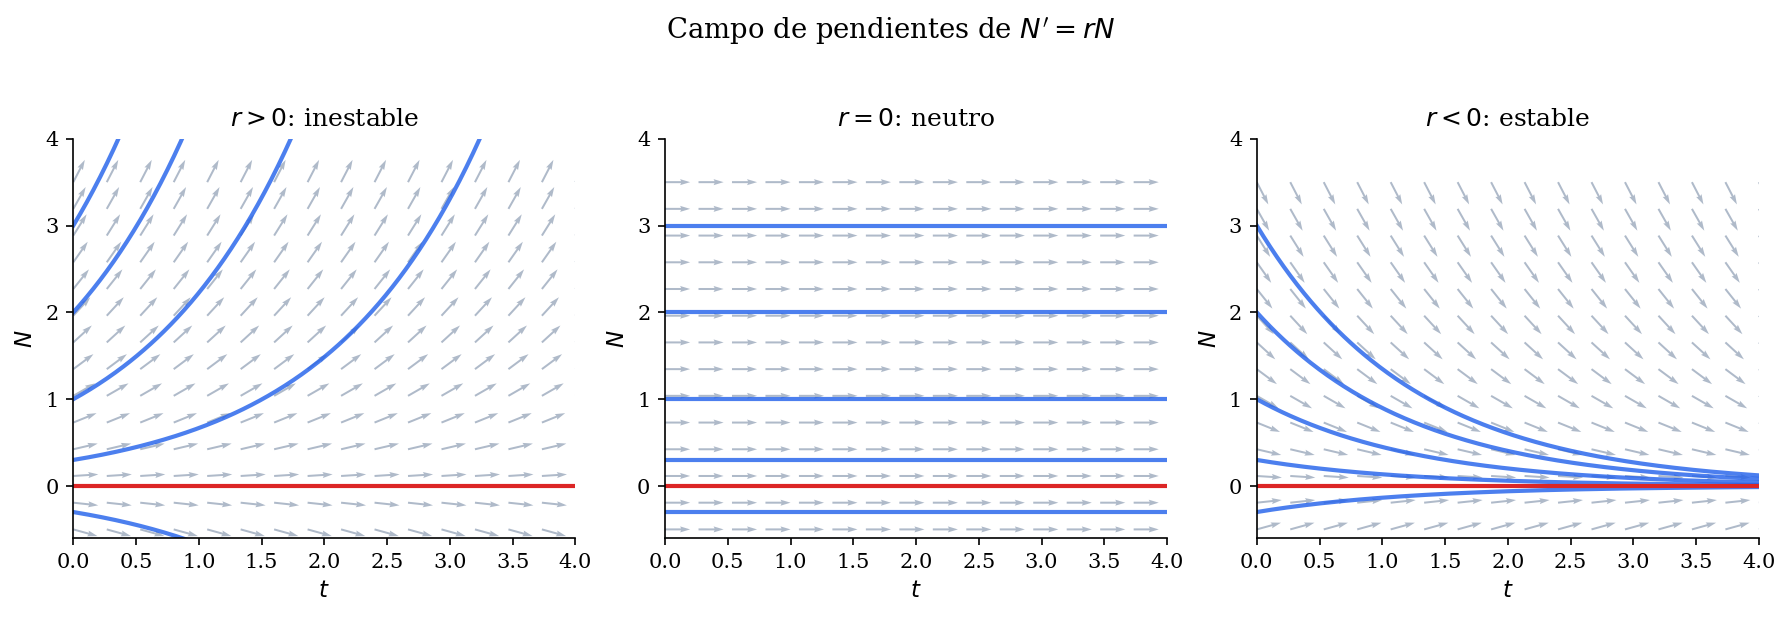
\includegraphics[width=0.92\textwidth]{fig_07_campo_malthusiano.png}
\caption{Campo de pendientes de $N'=rN$ para los tres casos cualitativos.}
\end{figure}

\subsection{Modelo con entrada y salida}

Con generación interna $\gamma$, mortalidad $m$ y entrada exterior $I$:
\[
\frac{dP}{dt}=(\gamma-m)P+I.
\]
El equilibrio es $P^*=I/(m-\gamma)$ (para $m\neq\gamma$) y la solución es
\[
P(t)=P^*+(P_0-P^*)e^{(\gamma-m)t}.
\]
Si $m>\gamma$ (la mortalidad supera la generación), el equilibrio es estable y
la población tiende a $P^*$ desde cualquier condición inicial.

% ============================================================
\section{Ecuaciones diferenciales autónomas}
% ============================================================

\begin{definicion}{Ecuación autónoma}{}
Una ecuación $\dfrac{dy}{dx}=f(y)$ donde el lado derecho \emph{no depende}
explícitamente de la variable independiente $x$ se llama \textbf{autónoma}.
\end{definicion}

La autonomía implica que el comportamiento cualitativo de las soluciones queda
completamente determinado por el signo de $f(y)$: no importa en qué ``instante''
se encuentre la solución, su tendencia depende solo de su valor actual.

\subsection{Puntos de equilibrio}

\begin{definicion}{Punto de equilibrio}{}
$y_0$ es un \textbf{punto de equilibrio} (o punto fijo) si $f(y_0)=0$.
La función constante $y(x)\equiv y_0$ es solución particular. Estas soluciones
constantes actúan como ``separatrices'' que organizan el espacio de fases.
\end{definicion}

\subsection{Línea de fase y análisis geométrico}

El signo de $f(y)$ determina la dirección del movimiento:
\[
f(y)>0\;\Rightarrow\; y'(x)>0\quad(\text{creciente});\qquad
f(y)<0\;\Rightarrow\; y'(x)<0\quad(\text{decreciente}).
\]

\textbf{Procedimiento estándar:}
\begin{enumerate}
    \item Encontrar los equilibrios: $f(y)=0$.
    \item Determinar el signo de $f(y)$ en los intervalos entre equilibrios.
    \item Construir la línea de fase con flechas.
    \item Clasificar cada equilibrio (estable, inestable, semiestable).
    \item Bosquejar cualitativamente las soluciones.
\end{enumerate}

\textbf{Clasificación geométrica:}
\begin{itemize}
    \item \textbf{Estable (atractor)}: flechas apuntan hacia $y_0$ desde ambos lados.
    \item \textbf{Inestable (repulsor)}: flechas se alejan de $y_0$ por ambos lados.
    \item \textbf{Semiestable}: un lado converge, el otro diverge.
\end{itemize}

\begin{figure}[H]
\centering
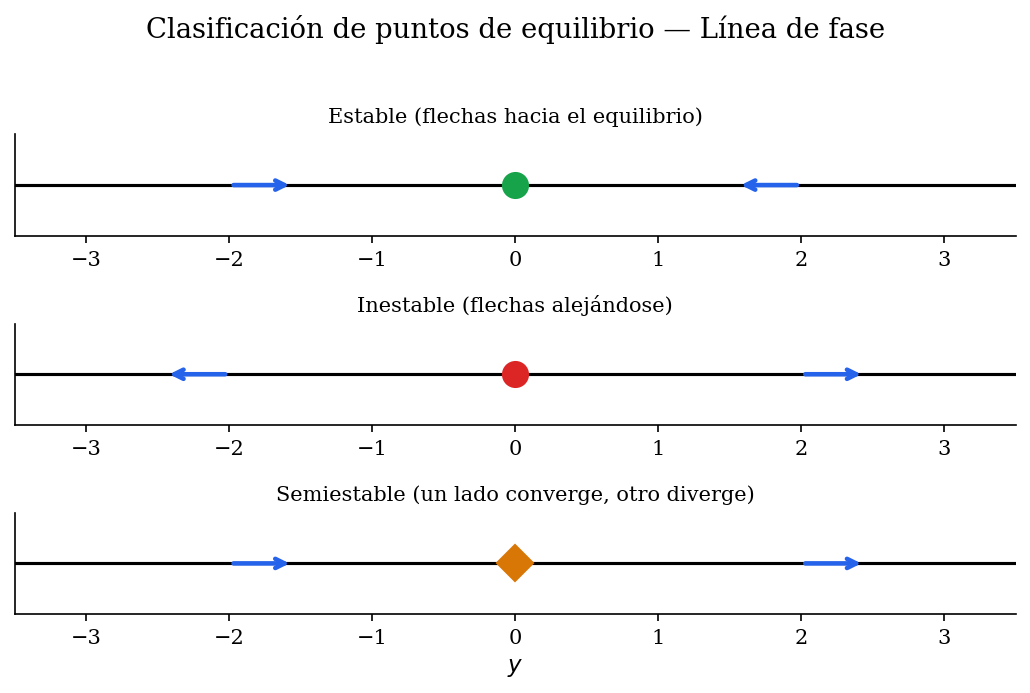
\includegraphics[width=0.74\textwidth]{fig_08_linea_fase_clasificacion.png}
\caption{Clasificación de equilibrios mediante la línea de fase.}
\end{figure}

% ============================================================
\section{Estabilidad y linealización}
% ============================================================

\subsection{Definiciones formales}

\begin{definicion}{Estabilidad de Lyapunov}{}
$y_0$ es \textbf{estable} si para todo $\varepsilon>0$ existe $\delta>0$
tal que $|y(0)-y_0|<\delta\Rightarrow|y(t)-y_0|<\varepsilon$ para todo $t\geq 0$.
En palabras: perturbaciones pequeñas producen desviaciones pequeñas para siempre.
\end{definicion}

\begin{definicion}{Estabilidad asintótica}{}
$y_0$ es \textbf{asintóticamente estable} si es estable y además
$|y(0)-y_0|<\delta\Rightarrow\lim_{t\to\infty}y(t)=y_0$.
La solución no solo permanece cerca sino que regresa al equilibrio.
\end{definicion}

\begin{figure}[H]
\centering
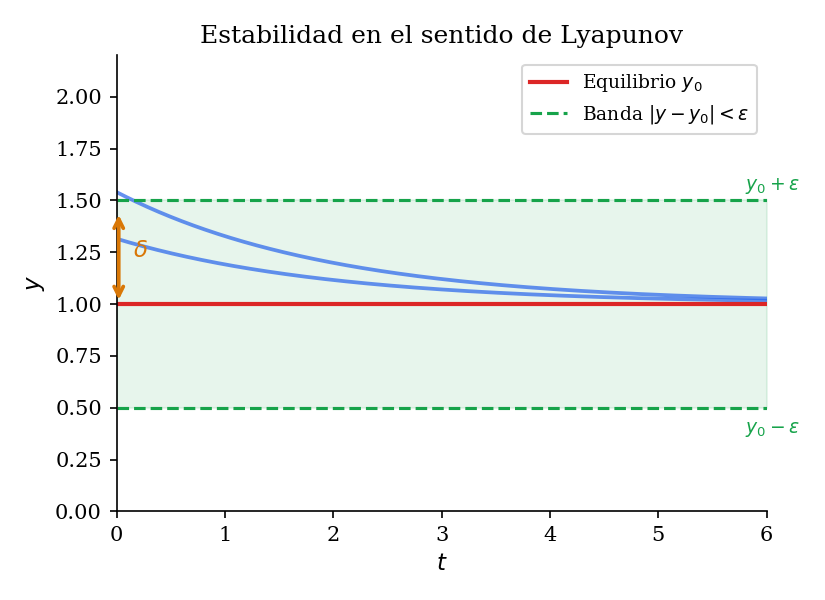
\includegraphics[width=0.62\textwidth]{fig_12_estabilidad_lyapunov.png}
\caption{Estabilidad de Lyapunov: trayectorias iniciadas dentro de la bola $\delta$
permanecen en la bola $\varepsilon$ para todo tiempo.}
\end{figure}

\subsection{Criterio de linealización (caso escalar)}

La idea central es aproximar $f$ por su desarrollo de Taylor de primer orden
alrededor del equilibrio. Como $f(y_0)=0$:
\[
f(y)\approx f'(y_0)(y-y_0).
\]
Con el cambio de variable $u(t)=y(t)-y_0$ (desplazamiento desde el equilibrio):
\[
u'\approx f'(y_0)u\;\Rightarrow\; u(t)=u(0)e^{f'(y_0)t}.
\]
Si $f'(y_0)<0$ el exponente es negativo y $u(t)\to 0$; si $f'(y_0)>0$ la
perturbación crece. Esto motiva el siguiente teorema:

\begin{teorema}{Criterio de linealización}{}
Sea $f\in C^1$ y $f(y_0)=0$. Entonces:
\begin{enumerate}[label=\alph*)]
    \item $f'(y_0)<0$: $y_0$ es \textbf{asintóticamente estable}.
    \item $f'(y_0)>0$: $y_0$ es \textbf{inestable}.
    \item $f'(y_0)=0$: el criterio no decide; se requiere análisis geométrico
          o términos de orden superior.
\end{enumerate}
\end{teorema}

\subsection{Expansión de Taylor en una y dos dimensiones}
\label{sec:taylor-multivariable}

La linealización en sistemas planos requiere entender primero la expansión de
Taylor para funciones vectoriales. Recordamos el caso escalar:
\[
f(x)\simeq f(x_0)+f'(x_0)(x-x_0)+\frac{1}{2}f''(x_0)(x-x_0)^2+\cdots
\]

\begin{figure}[H]
\centering
\begin{tikzpicture}[scale=0.95]
  \begin{scope}
    \draw[->] (-0.2,0) -- (4.2,0) node[right] {$x$};
    \draw[->] (0,-0.2) -- (0,2.1) node[above] {$y$};
    \draw[red!80!black,thick] (0.5,1.2) -- (3.5,1.2);
    \draw[dashed] (1.1,0) -- (1.1,1.2);
    \draw[dashed] (2.0,0) -- (2.0,1.2);
    \draw[dashed] (2.9,0) -- (2.9,1.2);
    \node[below] at (1.1,0) {$x_0-\varepsilon$};
    \node[below] at (2.0,0) {$x_0$};
    \node[below] at (2.9,0) {$x_0+\varepsilon$};
    \node[red!80!black] at (2.0,1.55) {$f(x)\simeq f(x_0)$};
  \end{scope}
  \begin{scope}[xshift=6.0cm]
    \draw[->] (-0.2,0) -- (4.2,0) node[right] {$x$};
    \draw[->] (0,-0.2) -- (0,2.1) node[above] {$y$};
    \draw[blue!70!black,thick] plot[smooth] coordinates {(0.4,0.45) (0.9,0.78) (1.4,1.02) (1.9,1.20) (2.4,1.30) (2.9,1.42) (3.4,1.56)};
    \draw[red!80!black,thick] (0.6,0.55) -- (3.3,1.78);
    \fill (1.9,1.20) circle (0.04) node[below right] {$x_0$};
    \draw[dashed] (1.9,0) -- (1.9,1.20);
    \node[red!80!black] at (2.7,1.9) {\small$f(x_0)+f'(x_0)(x-x_0)$};
  \end{scope}
\end{tikzpicture}
\caption{Izquierda: aproximación de orden cero (constante local). Derecha: aproximación
de primer orden (tangente), que captura la pendiente y es la base de la linealización.}
\end{figure}

Para un campo vectorial $F:\mathbb{R}^2\to\mathbb{R}^2$ de clase $C^\infty$
con $F=(F_1,F_2)$, tomando $x_0=(x_0,y_0)$, $h=x-x_0$, $k=y-y_0$, la expansión es:
\[
F(x_0+h,\, y_0+k)=F(x_0,y_0)+DF(x_0,y_0)\binom{h}{k}+O(\|(h,k)\|^2),
\]
donde la \textbf{matriz jacobiana} es
\[
DF(x_0,y_0)=J(x_0,y_0)=
\begin{pmatrix}
\dfrac{\partial F_1}{\partial x}(x_0,y_0) & \dfrac{\partial F_1}{\partial y}(x_0,y_0)\\[1ex]
\dfrac{\partial F_2}{\partial x}(x_0,y_0) & \dfrac{\partial F_2}{\partial y}(x_0,y_0)
\end{pmatrix}.
\]
Si $x_0$ es un punto de equilibrio, $F(x_0)=\vec{0}$, y la primera aproximación
significativa es el término lineal. Esto justifica estudiar el sistema linealizado
$Y'=DF(x_0)Y$ para entender el comportamiento local.

\begin{figure}[H]
\centering
\begin{tikzpicture}[scale=1]
  \draw[->] (-0.2,0) -- (4.8,0) node[right] {$x$};
  \draw[->] (0,-0.2) -- (0,4.0) node[above] {$y$};
  \draw[dashed,gray] (1.4,2.0) circle (1.1);
  \fill (1.4,2.0) circle (0.05) node[above right] {$x_0$};
  \draw[->,thick] (1.4,2.0) -- (2.2,2.45) node[midway,above] {$h$};
  \fill (2.2,2.45) circle (0.04) node[right] {$x_0+h$};
  \node at (3.15,3.05) {$F(x_0+h)\simeq F(x_0)+DF(x_0)h$};
\end{tikzpicture}
\caption{Esquema de linealización local: en una vecindad de $x_0$,
el campo no lineal $F$ se aproxima por el mapa lineal $DF(x_0)$.}
\end{figure}

\subsection{Linealización en sistemas planos}

Para un sistema autónomo $x'=P(x,y)$, $y'=Q(x,y)$ con equilibrio $X_0=(x_0,y_0)$,
el sistema linealizado alrededor de $X_0$ es $Y'=J(X_0)Y$ donde
\[
J(x,y)=\begin{pmatrix}
\partial P/\partial x & \partial P/\partial y\\
\partial Q/\partial x & \partial Q/\partial y
\end{pmatrix}.
\]

\textbf{Ejemplo de linealización.} Consideremos el sistema
\begin{align*}
x' &= x^2-y^2-1,\\
y' &= 2y.
\end{align*}
El jacobiano es
\[
J(x,y)=\begin{pmatrix}2x & -2y\\ 0 & 2\end{pmatrix}.
\]
Los puntos de equilibrio satisfacen $x^2-y^2-1=0$ y $2y=0$. De $y=0$:
$x^2=1$, así que hay dos equilibrios: $X_0=(1,0)$ y $X_1=(-1,0)$.

\begin{figure}[H]
\centering
\begin{tikzpicture}[scale=1.05,>=Stealth]
  \draw[->] (-2.5,0) -- (2.5,0) node[right] {$x$};
  \draw[->] (0,-2.5) -- (0,2.5) node[above] {$y$};
  \foreach \x in {-2,-1.5,...,2} {
    \foreach \y in {-2,-1.5,...,2} {
      \pgfmathsetmacro{\u}{\x*\x - \y*\y - 1}
      \pgfmathsetmacro{\v}{2*\y}
      \pgfmathsetmacro{\nrm}{max(0.35,sqrt(\u*\u+\v*\v))}
      \draw[blue!70,->,line width=0.35pt,opacity=0.9]
        (\x,\y) -- ++({0.22*\u/\nrm},{0.22*\v/\nrm});
    }
  }
  \draw[yellow!85!orange,thick] (-2.35,0) -- (2.35,0);
  \draw[orange!85!red,thick] plot[domain=1:2.25,samples=120] (\x,{sqrt(\x*\x-1)});
  \draw[orange!85!red,thick] plot[domain=1:2.25,samples=120] (\x,{-sqrt(\x*\x-1)});
  \draw[orange!85!red,thick] plot[domain=-2.25:-1,samples=120] (\x,{sqrt(\x*\x-1)});
  \draw[orange!85!red,thick] plot[domain=-2.25:-1,samples=120] (\x,{-sqrt(\x*\x-1)});
  \fill[black] (1,0) circle (0.05);
  \fill[black] (-1,0) circle (0.05);
  \node[black,below right] at (1,0) {$(1,0)$};
  \node[black,below left] at (-1,0) {$(-1,0)$};
\end{tikzpicture}
\caption{Campo vectorial del sistema $x'=x^2-y^2-1$, $y'=2y$. Las curvas
naranjas son las nullclines ($x'=0$), la amarilla el eje $x$ ($y'=0$).
Los puntos de equilibrio se ubican en las intersecciones.}
\end{figure}

% ============================================================
\section{Modelo logístico}
\label{sec:modelo-logistico}
% ============================================================

El modelo malthusiano es irrealista para tiempos largos porque la población
crecería sin límite. El modelo logístico corrige esto introduciendo la
\emph{capacidad de carga} $K>0$: el término $(1-N/K)$ hace que el crecimiento
disminuya conforme la población se acerca al límite del entorno:
\[
\boxed{\frac{dN}{dt}=rN\!\left(1-\frac{N}{K}\right),\qquad r,K>0.}
\]

\subsection{Puntos de equilibrio}

$f(N)=rN(1-N/K)=0\;\Rightarrow\;N_0=0$ (extinción, inestable) y $N_1=K$
(capacidad de carga, estable).

\subsection{Análisis geométrico}

\begin{itemize}
    \item $0<N<K$: $f(N)>0$ $\Rightarrow$ $N$ crece hacia $K$.
    \item $N>K$: $f(N)<0$ $\Rightarrow$ $N$ decrece hacia $K$.
\end{itemize}
Las soluciones con $N_0>0$ siempre tienden a $K$; la curva solución tiene
forma sigmoidal.

\begin{figure}[H]
\centering
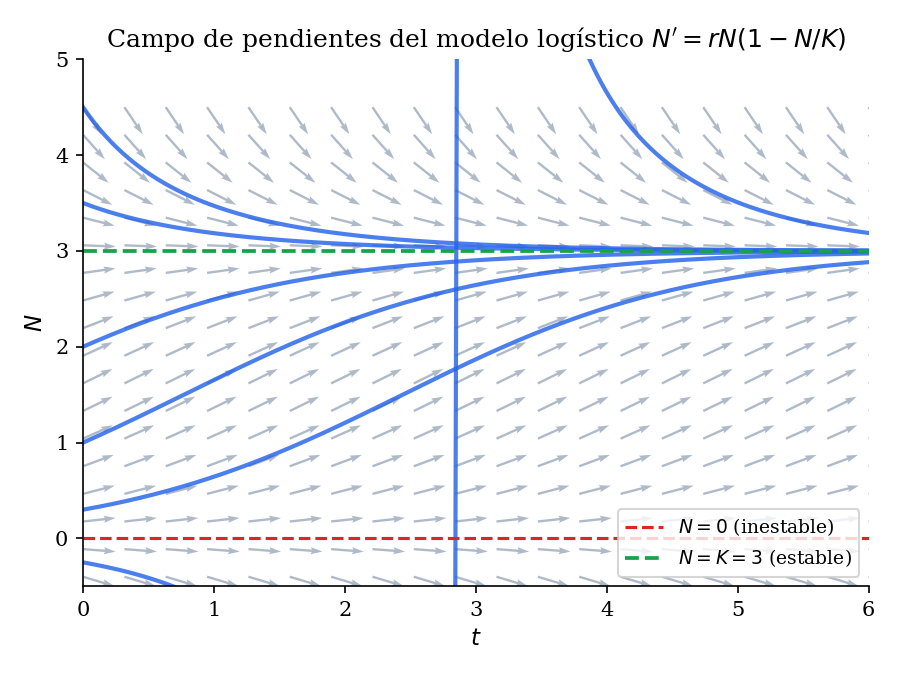
\includegraphics[width=0.72\textwidth]{fig_09_campo_logistico.png}
\caption{Campo de pendientes del logístico. Soluciones sigmoidales convergen a $K$
desde abajo o desde arriba.}
\end{figure}

\begin{figure}[H]
\centering
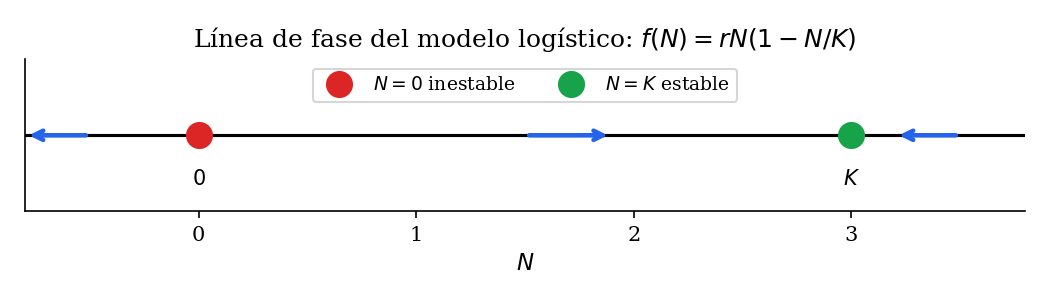
\includegraphics[width=0.70\textwidth]{fig_10_linea_fase_logistico.png}
\caption{Línea de fase: $N=0$ es inestable; $N=K$ es asintóticamente estable.}
\end{figure}

\subsection{Linealización}

$f'(N)=r-2rN/K$.
\[
f'(0)=r>0\;\Rightarrow\; N=0\text{ inestable}.\qquad
f'(K)=-r<0\;\Rightarrow\; N=K\text{ a.e.}
\]

\subsection{Solución analítica}

La ecuación es separable. Con fracciones parciales:
\[
\frac{K}{N(K-N)}=\frac{1}{N}+\frac{1}{K-N},
\]
integrando y usando $N(0)=N_0$ se obtiene la solución sigmoidal exacta:
\[
\boxed{N(t)=\frac{K}{1+\displaystyle\left(\frac{K-N_0}{N_0}\right)e^{-rt}}.}
\]

Una vez resuelto el caso base, conviene mirar dos extensiones muy comunes:
la extracción constante y el efecto Allee. Ambas conservan la misma lógica de
equilibrios, pero cambian de forma importante la estabilidad.

\subsection{Modelo logístico con cosecha}

Con extracción constante $H>0$:
\[
\frac{dN}{dt}=rN\!\left(1-\frac{N}{K}\right)-H.
\]
Los equilibrios satisfacen $N^*=\dfrac{K}{2}\!\left(1\pm\sqrt{1-4H/(rK)}\right)$.
Hay tres regímenes: si $H<rK/4$ existen dos equilibrios (uno estable, uno
inestable); si $H=rK/4$ los equilibrios coinciden en una bifurcación silla-nodo;
si $H>rK/4$ no hay equilibrios y la población colapsa.

\begin{figure}[H]
\centering
\begin{tikzpicture}
\begin{axis}[
    width=0.94\textwidth, height=5.2cm,
    xmin=0, xmax=0.40, ymin=-0.05, ymax=1.05,
    axis lines=middle,
    xlabel={$\lambda=H/(rK)$}, ylabel={$u^*=N/K$},
    title={Bifurcación silla-nodo del logístico con cosecha},
    samples=200, tick style={draw=none}
]
\addplot[thick,blue!75!black,domain=0:0.249] ({x},{0.5 - sqrt(0.25 - x)});
\addplot[thick,blue!75!black,domain=0:0.249] ({x},{0.5 + sqrt(0.25 - x)});
\addplot[thick,red!70!black,dashed] coordinates {(0.25,0) (0.25,1)};
\node[anchor=west] at (axis cs:0.258,0.95) {$\lambda=\frac14$};
\end{axis}
\end{tikzpicture}
\caption{Diagrama de bifurcación silla-nodo: los dos equilibrios colisionan y desaparecen
en $\lambda=H/(rK)=1/4$. Para $\lambda>1/4$ no hay equilibrios positivos.}
\end{figure}

\subsection{Modelo logístico con efecto Allee}

El efecto Allee ocurre cuando poblaciones muy pequeñas tienen dificultad para
reproducirse (por ejemplo, falta de parejas). Si el crecimiento neto cambia
de signo por debajo de un umbral $A$:
\[
\frac{dN}{dt}=rN\!\left(1-\frac{N}{K}\right)\!\left(\frac{N}{A}-1\right),
\qquad r>0,\; 0<A<K.
\]
Equilibrios: $N_0=0$ (estable), $N_1=A$ (inestable, umbral crítico), $N_2=K$ (estable).
Si la población cae por debajo de $A$, la extinción es inevitable.

\begin{figure}[H]
\centering
\begin{tikzpicture}
\begin{axis}[
    width=0.92\textwidth, height=6cm,
    xmin=0, xmax=2, ymin=-0.05, ymax=1.15,
    axis lines=middle,
    xlabel={$\lambda=A/K$}, ylabel={$u^*=N/K$},
    tick style={draw=none},
    title={Bifurcación transcrítica del efecto Allee},
    samples=200
]
\addplot[thick,blue!70!black,domain=0:2] {0};
\addplot[thick,blue!70!black,domain=0:1] {1};
\addplot[thick,blue!70!black,dashed,domain=1:2] {1};
\addplot[thick,blue!70!black,dashed,domain=0:1] {x};
\addplot[thick,blue!70!black,domain=1:2] {x};
\addplot[only marks,mark=*,mark size=1.5pt] coordinates {(1,1)};
\end{axis}
\end{tikzpicture}
\caption{Las ramas no triviales intercambian estabilidad en $\lambda=A/K=1$.
         Para $A<K$ el umbral $A$ es inestable y $K$ es estable.}
\end{figure}

% ============================================================
\section{Bifurcaciones en sistemas unidimensionales}
\label{sec:bifurcaciones-unidim}
% ============================================================

Los dos ejemplos anteriores muestran que, al variar un parámetro, los puntos de
equilibrio pueden aparecer, desaparecer o intercambiar estabilidad. Esta es la
idea central de una \emph{bifurcación}: un cambio cualitativo en la estructura
de los equilibrios al cruzar un valor crítico del parámetro.

\begin{definicion}{Bifurcación}{}
Se dice que $\mu_0$ es un \textbf{valor de bifurcación} de $y'=f(y,\mu)$
si al cruzar $\mu_0$ cambia el número o la estabilidad de los equilibrios.
\end{definicion}

El \textbf{diagrama de bifurcación} grafica los equilibrios $y^*(\mu)$ en el
plano $(\mu,y^*)$, usando línea sólida para ramas estables y línea discontinua
para inestables.

\subsection{Bifurcación silla-nodo}

Dos equilibrios (uno estable, uno inestable) se crean o destruyen al variar $\mu$.

\textbf{Ejemplo canónico:} $y'=y^2+\mu$.
\begin{itemize}
    \item $\mu<0$: equilibrios $y^*=\pm\sqrt{-\mu}$; $y^*=-\sqrt{-\mu}$ estable, $y^*=\sqrt{-\mu}$ inestable.
    \item $\mu=0$: único equilibrio $y^*=0$ semiestable (bifurcación).
    \item $\mu>0$: no hay equilibrios.
\end{itemize}
Verificación por linealización: $f'(y)=2y$, de modo que
$f'(-\sqrt{-\mu})=-2\sqrt{-\mu}<0$ (estable) y $f'(\sqrt{-\mu})=2\sqrt{-\mu}>0$ (inestable).

\textbf{Variante:} $y'=\mu+y-y^3$. Los equilibrios satisfacen $\mu=y^3-y$.
Para ciertos rangos de $\mu$ coexisten tres soluciones; hay dos valores de
bifurcación silla-nodo donde la curva $\mu=y^3-y$ tiene extremos locales.

\subsection{Bifurcación transcrítica}

Dos equilibrios existen para todo $\mu$ pero \emph{intercambian estabilidad}
al cruzar $\mu_0$.

\textbf{Ejemplo canónico:} $y'=\mu y-y^2=y(\mu-y)$.
\begin{itemize}
    \item Equilibrios: $y^*=0$ y $y^*=\mu$ para todo $\mu$.
    \item $f'(y)=\mu-2y$.
    \item $\mu<0$: $f'(0)=\mu<0$ ($y=0$ estable); $f'(\mu)=-\mu>0$ ($y=\mu$ inestable).
    \item $\mu>0$: $f'(0)=\mu>0$ ($y=0$ inestable); $f'(\mu)=-\mu<0$ ($y=\mu$ estable).
    \item $\mu=0$: ambos equilibrios coinciden; linealización no decide.
\end{itemize}

\subsection{Bifurcación pitchfork supercrítica}

Un equilibrio estable se divide en tres al cruzar $\mu_0$: el central se
vuelve inestable y nacen dos nuevos estables.

\textbf{Ejemplo canónico:} $y'=\mu y-y^3$.
\begin{itemize}
    \item Equilibrios: $y^*=0$ y (para $\mu>0$) $y^*=\pm\sqrt{\mu}$.
    \item $f'(y)=\mu-3y^2$.
    \item $\mu\leq 0$: $f'(0)=\mu\leq 0$; solo $y=0$, estable.
    \item $\mu>0$: $f'(0)=\mu>0$ ($y=0$ inestable); $f'(\pm\sqrt{\mu})=-2\mu<0$ (estables).
\end{itemize}
El nombre ``supercrítica'' indica que las ramas nuevas aparecen del lado $\mu>0$.

\subsection{Bifurcación pitchfork subcrítica}

\textbf{Ejemplo canónico:} $y'=\mu y+y^3$.
\begin{itemize}
    \item Equilibrios: $y^*=0$ y (para $\mu<0$) $y^*=\pm\sqrt{-\mu}$.
    \item $f'(y)=\mu+3y^2$.
    \item $\mu<0$: $f'(0)=\mu<0$ ($y=0$ estable); $f'(\pm\sqrt{-\mu})=-2\mu>0$
          ($y^*=\pm\sqrt{-\mu}$ \emph{inestables}).
    \item $\mu>0$: $f'(0)=\mu>0$ ($y=0$ inestable); no hay equilibrios adicionales.
\end{itemize}
Las ramas inestables existen para $\mu<0$. El sistema presenta \emph{histéresis}:
al aumentar $\mu$ más allá de cero, el sistema salta bruscamente de forma irreversible.

\subsection{Tipos de bifurcaciones}

\begin{center}
\begin{tabular}{lll}
\toprule
Tipo & Ejemplo & Característica\\
\midrule
Silla-nodo & $y'=y^2+\mu$ & se crean/destruyen 2 equilibrios\\
Transcrítica & $y'=\mu y-y^2$ & intercambio de estabilidad\\
Pitchfork supercrítica & $y'=\mu y-y^3$ & bifurcación con simetría $y\leftrightarrow -y$\\
Pitchfork subcrítica & $y'=\mu y+y^3$ & ramas inestables; histéresis\\
Bifurcación periódica & $\dot\theta=\mu\sin\theta$ & infinitos equilibrios periódicos\\
Cúspide (codim.~2) & $y'=y^3-3\mu y+\mu$ & requiere dos parámetros\\
\bottomrule
\end{tabular}
\end{center}

\subsection{Bifurcación periódica: flujos en el círculo}

Cuando la variable de estado es un \emph{ángulo} $\theta\in[0,2\pi)$, el espacio
de fases es el \textbf{círculo}, y las soluciones pueden ser periódicas aunque
el sistema sea unidimensional (Strogatz, Cap.~4).

\begin{definicion}{Campo vectorial en el círculo}{}
Una ecuación $\dot\theta=f(\theta)$ donde $f$ es $2\pi$-periódica define un
\textbf{campo vectorial en el círculo}. A diferencia de la recta, una partícula
puede regresar a su punto de partida, generando soluciones periódicas.
\end{definicion}

\textbf{Ejemplo canónico:} $\dot\theta=\mu\sin\theta$.
\begin{itemize}
  \item Los equilibrios satisfacen $\sin\theta^*=0$: $\theta^*=0$ y $\theta^*=\pi$.
  \item $f'(\theta)=\mu\cos\theta$: en $\theta^*=0$, $f'(0)=\mu$; en $\theta^*=\pi$, $f'(\pi)=-\mu$.
  \item Al cruzar $\mu=0$ los dos equilibrios intercambian estabilidad (bifurcación transcrítica en el círculo).
\end{itemize}

\begin{observacion}{Multiplicidad periódica}{}
Como $f(\theta)=\mu\sin\theta$ es $2\pi$-periódica, en el círculo hay infinitos
equilibrios: $\theta^*=k\pi$, $k\in\mathbb{Z}$, que intercambian estabilidad
simultáneamente al cruzar $\mu=0$.
\end{observacion}

\subsection{Bifurcación de cúspide (codimensión 2)}

Todos los tipos anteriores son de codimensión~1: basta variar un solo parámetro.
La \textbf{cúspide} es de codimensión~2: se necesitan dos parámetros (Strogatz, §3.6).

\textbf{Forma normal:} $\dot{x} = h + rx - x^3$, con parámetros $r$ (bifurcación)
y $h$ (imperfección). Los equilibrios satisfacen $x^3-rx=h$.
\begin{itemize}
    \item $r\leq 0$: exactamente \textbf{1 equilibrio} para todo $h$.
    \item $r>0$, $|h|<h_c(r)$: \textbf{3 equilibrios}; $|h|=h_c(r)$: bifurcación silla-nodo; $|h|>h_c(r)$: 1 equilibrio.
\end{itemize}
Al variar $h$ con $r>0$ fijo, el sistema puede exhibir \textbf{histéresis}: los
saltos de ida y vuelta ocurren en valores distintos de $h$, generando la
\emph{catástrofe de cúspide}.

% ============================================================
\section{Ejemplo: \texorpdfstring{$y'=y^2+\alpha$}{y' = y² + alpha}}
% ============================================================

\[
\frac{dy}{dx}=y^2+\alpha,\qquad\alpha\in\mathbb{R}.
\]
\textbf{$\alpha<0$:} equilibrios $y_1=-\sqrt{-\alpha}$ (estable) y $y_2=\sqrt{-\alpha}$ (inestable).
\textbf{$\alpha=0$:} único equilibrio $y=0$ semiestable.
\textbf{$\alpha>0$:} no hay equilibrios; todas las soluciones crecen indefinidamente.

\begin{figure}[H]
\centering
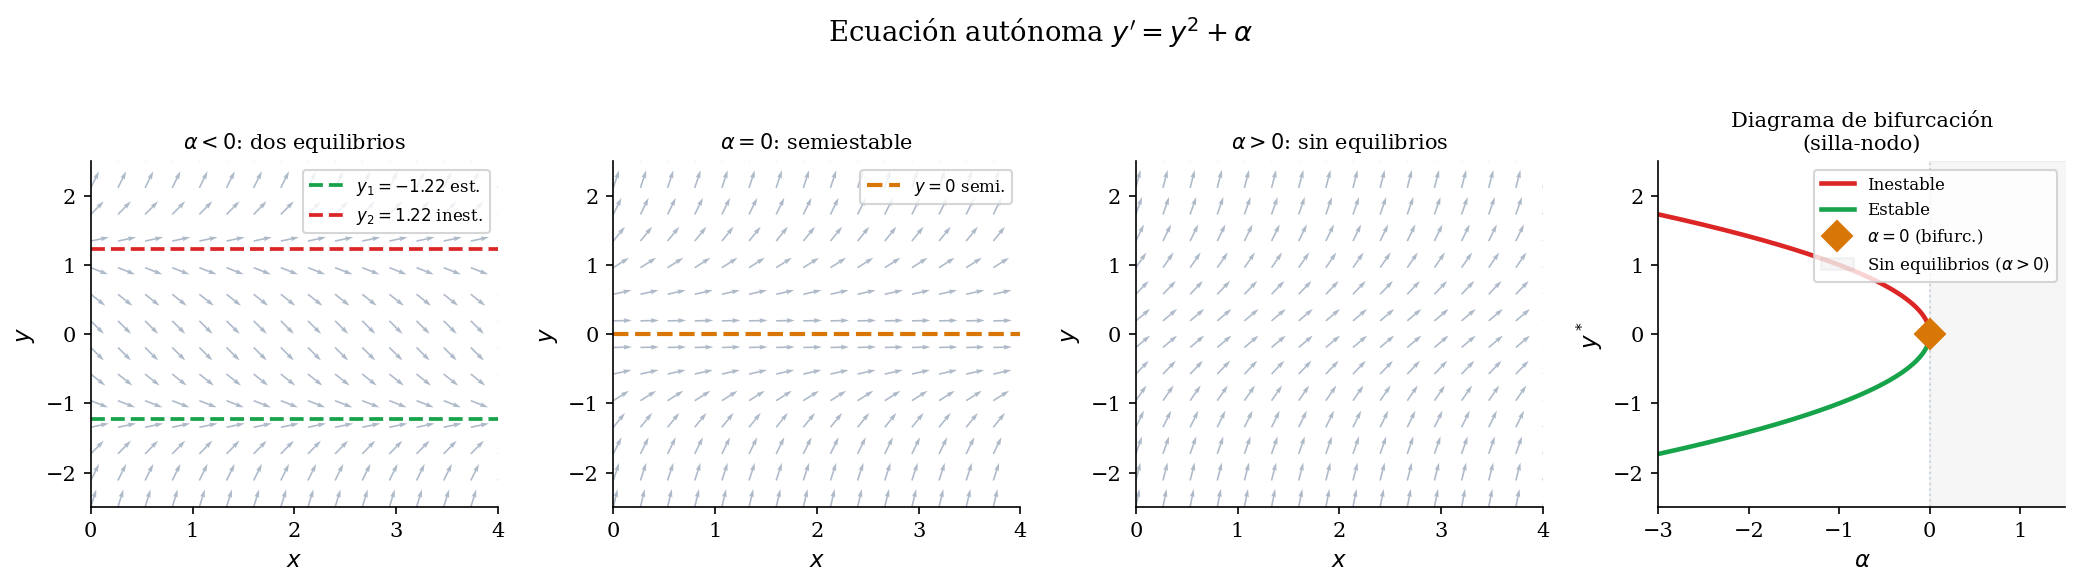
\includegraphics[width=\textwidth]{fig_11_autonoma_bifurcacion.png}
\caption{Campos de pendientes y diagrama de bifurcación silla-nodo de $y'=y^2+\alpha$.}
\end{figure}

% ============================================================
\section{Adimensionalización}
\label{sec:adimensionalizacion}
% ============================================================

La \textbf{adimensionalización} es el proceso de eliminar unidades físicas
mediante cambios de variable apropiados, reduciendo el número de parámetros
relevantes. La idea es que la dinámica esencial de muchos sistemas distintos
está gobernada por la misma estructura matemática.

\begin{definicion}{Análisis dimensional}{}
Una ecuación diferencial está \textbf{adimensionalizada} si todas sus variables
y parámetros son adimensionales (dimensión~1, sin unidades).
\end{definicion}

\textbf{Procedimiento general:}
\begin{enumerate}
    \item Identificar variables y parámetros con dimensiones.
    \item Construir escalas características $x_c$, $t_c$, etc., a partir de los parámetros.
    \item Definir variables adimensionales: $\hat{x}=x/x_c$, $\hat{t}=t/t_c$.
    \item Sustituir y verificar que el resultado no tiene unidades.
    \item Identificar los parámetros adimensionales que controlan la dinámica.
\end{enumerate}

\subsection{Análisis dimensional del modelo logístico}

Para $dN/dt=rN(1-N/K)$: $[N]=[K]=\mathcal{N}$, $[r]=T^{-1}$, $[t]=T$.
Con $u=N/K$ y $\tau=rt$:
\[
\frac{du}{d\tau}=u(1-u).
\]
Esta ecuación no tiene parámetros: todos fueron absorbidos por las escalas.

\subsection{Adimensionalización del logístico con cosecha}

Con $u=N/K$ y $\tau=rt$:
\[
\frac{du}{d\tau}=u(1-u)-\lambda,\qquad \lambda=\frac{H}{rK}.
\]

\subsection{Adimensionalización del efecto Allee}

Con $u=N/K$ y $\tau=rt$:
\[
\frac{du}{d\tau}=u(1-u)\!\left(\frac{u}{\lambda}-1\right),
\qquad \lambda=\frac{A}{K}.
\]

\subsection{Caída libre con resistencia lineal \naglecite{§3.4}}

Una partícula de masa $m$ cae bajo gravedad con resistencia proporcional a la velocidad:
\[
m\frac{dv}{dt}=mg-kv,\qquad k>0.
\]
Velocidad terminal: $v_\infty=mg/k$. Tiempo característico: $t_c=m/k$.
Con $\hat{v}=v/v_\infty$ y $\hat{t}=t/t_c$:
\[
\boxed{\frac{d\hat{v}}{d\hat{t}}=1-\hat{v}.}
\]
La ecuación no tiene parámetros y es idéntica a la del circuito RC adimensionalizado,
evidenciando la equivalencia estructural entre los dos sistemas.

\subsection{Oscilador armónico amortiguado \naglecite{§4.1, §4.9}}

Masa $m$, resorte $k$, amortiguamiento $c\geq 0$:
\[
m\frac{d^2x}{dt^2}+c\frac{dx}{dt}+kx=0.
\]
Con $\omega_0=\sqrt{k/m}$, $\hat{x}=x/x_c$, $\tau=\omega_0 t$:
\[
\boxed{\frac{d^2\hat{x}}{d\tau^2}+2\zeta\frac{d\hat{x}}{d\tau}+\hat{x}=0,}
\qquad \zeta=\frac{c}{2\sqrt{mk}}.
\]
El único parámetro adimensional $\zeta$ clasifica el comportamiento:
$\zeta<1$ (subamortiguado, oscilaciones decrecientes), $\zeta=1$ (críticamente amortiguado),
$\zeta>1$ (sobreamortiguado, sin oscilaciones).

\subsection{Péndulo simple \naglecite{§4.8}}

El ángulo $\theta(t)$ satisface:
\[
\frac{d^2\theta}{dt^2}+\frac{g}{L}\sin\theta=0.
\]
Con $\tau=t\sqrt{g/L}$:
\[
\boxed{\frac{d^2\theta}{d\tau^2}+\sin\theta=0.}
\]
La ecuación adimensionalizada no tiene parámetros. El período de oscilaciones
pequeñas ($\sin\theta\approx\theta$) en $\tau$ es $2\pi$, correspondiente al
período dimensional $T=2\pi\sqrt{L/g}$.

% ============================================================
\section{Normalización del modelo logístico}
\label{sec:normalizacion-logistica}
% ============================================================

Con $u=N/K$ y $\tau=rt$ el logístico se reduce a $\dot{u}=u(1-u)$. Este
resultado concentra la normalización que elimina $r$ y $K$ simultáneamente
y deja una ecuación universal.

\begin{figure}[H]
\centering
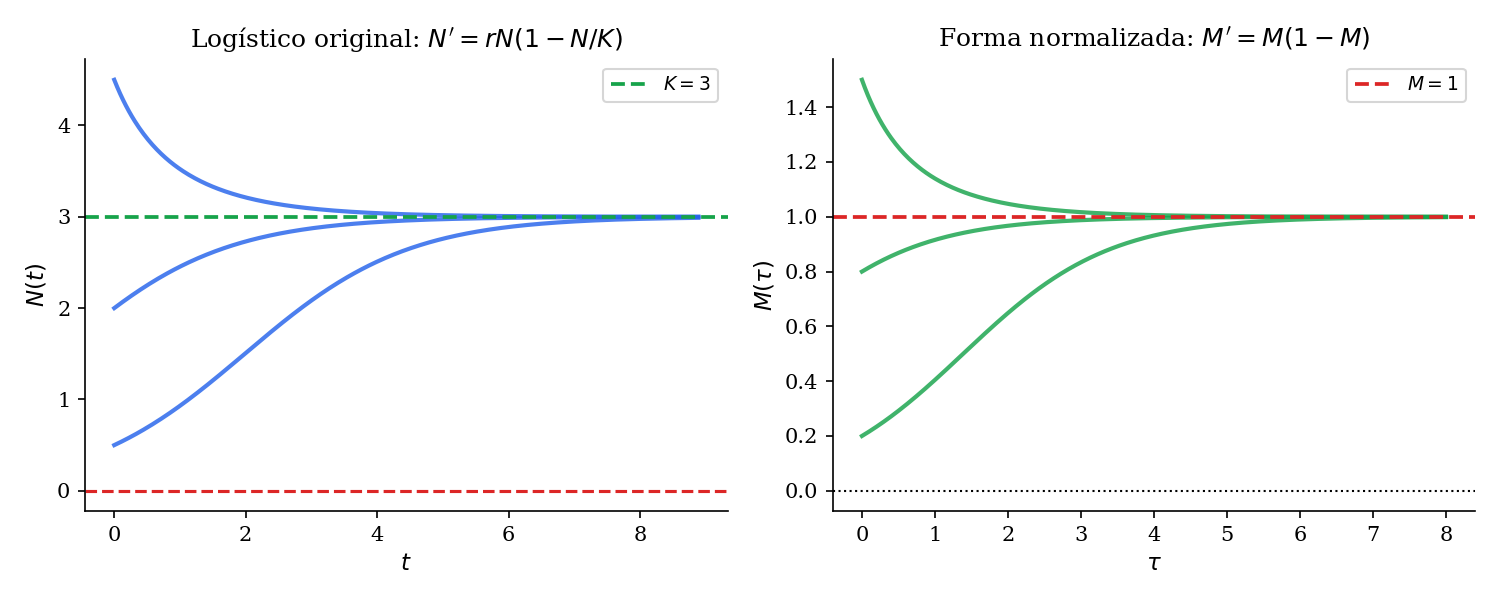
\includegraphics[width=0.88\textwidth]{fig_13_normalizacion_logistica.png}
\caption{Izquierda: logístico original $N'=rN(1-N/K)$.
Derecha: forma normalizada $\dot{u}=u(1-u)$ con $u=N/K$, $\tau=rt$.}
\end{figure}

\subsection{Análisis dimensional comparado}

\begin{center}
\begin{tabular}{lll}
\toprule
Ecuación & Variables con dimensión & Parámetros adimensionales\\
\midrule
$N'=rN(1-N/K)$ & $N$ ($\mathcal{N}$), $t$ ($T$) & $r$ ($T^{-1}$), $K$ ($\mathcal{N}$)\\
$\dot{u}=u(1-u)$ & --- & ninguno\\
$\dot{u}=u(1-u)-\lambda$ & --- & $\lambda=H/(rK)$\\
$\dot{u}=u(1-u)(u/\lambda-1)$ & --- & $\lambda=A/K$\\
\bottomrule
\end{tabular}
\end{center}

% ============================================================
\section{Sistemas lineales: \texorpdfstring{$\vec{X}'=A\vec{X}$}{X' = AX}}
\label{sec:sistemas-lineales}
% ============================================================

Dado un sistema lineal con coeficientes constantes
\[
\vec{X}'=A\vec{X},\qquad A\in M_{n\times n}(\mathbb{R}),
\]
el caso escalar $x'=ax$ tiene solución $x(t)=x_0e^{at}$. La idea es extender
este \emph{ansatz} exponencial al caso vectorial.

\subsection{El ansatz exponencial y los valores propios}

Proponemos una solución de la forma $X(t)=e^{\lambda t}v$ con
$\lambda\in\mathbb{R}$ y $v\in\mathbb{R}^n$. Calculando la derivada:
\[
X'(t)=\lambda e^{\lambda t}v.
\]
Para que $X(t)$ sea solución del sistema necesitamos $X'(t)=AX(t)$, es decir,
\[
\lambda e^{\lambda t}v = e^{\lambda t}Av \quad \Longrightarrow \quad Av=\lambda v.
\]
Por lo tanto, $X(t)=e^{\lambda t}v$ es solución \textbf{si y solo si} $\lambda$
es valor propio de $A$ y $v$ es el vector propio correspondiente. El sistema lineal
queda así completamente vinculado al problema de valores propios de $A$.

\subsection{Solución general}

Si $A$ tiene $n$ valores propios distintos $\lambda_1,\lambda_2,\ldots,\lambda_n$
con vectores propios correspondientes $v_1,\ldots,v_n$, entonces estos últimos son
linealmente independientes. El conjunto
\[
\left\{X_j(t)=e^{\lambda_j t}v_j\right\}_{j=1}^n
\]
es un conjunto fundamental de soluciones, y la solución general es la combinación lineal:
\[
X(t)=\sum_{j=1}^n c_j e^{\lambda_j t}v_j.
\]

% ============================================================
\section{Dinámica local en el plano: tipos de equilibrios}
\label{sec:dinamica-local}
% ============================================================

Para un sistema autónomo $x'=F(x)$ con $F:\mathbb{R}^n\to\mathbb{R}^n$ de
clase $C^1$, la pregunta central de la dinámica local es: dado un punto
$x_0\in\mathbb{R}^n$, ¿cuál es el comportamiento de las soluciones cerca de $x_0$?
Hay dos posibilidades:

\begin{enumerate}
    \item \textbf{Punto regular}: $F(x_0)\neq\vec{0}$. Por el teorema de
          enderezamiento de flujos, localmente el campo se parece a uno constante:
          las órbitas son curvas casi paralelas que atraviesan $x_0$.
    \item \textbf{Punto de equilibrio}: $F(x_0)=\vec{0}$. Aquí la estructura
          local puede ser variada: el linealizado determina el tipo.
\end{enumerate}

En el plano ($n=2$), los tipos genéricos de equilibrios hiperbólicos son:

\begin{figure}[H]
\centering
\begin{tikzpicture}[scale=0.95,>=Stealth]
  \newcommand{\miniaxes}{
    \draw[->] (-1.4,0) -- (1.4,0);
    \draw[->] (0,-1.4) -- (0,1.4);
  }
  \begin{scope}[shift={(-4.3,2.0)}]
    \miniaxes
    \foreach \a in {0,30,...,330} {
      \draw[blue!70,->,line width=0.35pt] (0,0) -- ({1.05*cos(\a)},{1.05*sin(\a)});
    }
    \node[font=\small] at (0,-1.85) {Fuente ($\lambda_1,\lambda_2>0$)};
  \end{scope}
  \begin{scope}[shift={(0,2.0)}]
    \miniaxes
    \foreach \a in {0,30,...,330} {
      \draw[blue!70,->,line width=0.35pt] ({1.05*cos(\a)},{1.05*sin(\a)}) -- (0,0);
    }
    \node[font=\small] at (0,-1.85) {Sumidero ($\lambda_1,\lambda_2<0$)};
  \end{scope}
  \begin{scope}[shift={(4.3,2.0)}]
    \miniaxes
    \draw[red!75,->,line width=0.45pt] (-1.2,0) -- (-0.15,0);
    \draw[red!75,->,line width=0.45pt] (0.15,0) -- (1.2,0);
    \draw[blue!70,->,line width=0.45pt] (0,-1.2) -- (0,-0.15);
    \draw[blue!70,->,line width=0.45pt] (0,1.2) -- (0,0.15);
    \draw[blue!70,thick] plot[domain=-1.2:-0.25,samples=70] (\x,{0.65/\x});
    \draw[blue!70,thick] plot[domain=0.25:1.2,samples=70] (\x,{0.65/\x});
    \draw[blue!70,thick] plot[domain=-1.2:-0.25,samples=70] (\x,{-0.65/\x});
    \draw[blue!70,thick] plot[domain=0.25:1.2,samples=70] (\x,{-0.65/\x});
    \node[font=\small] at (0,-1.85) {Silla ($\lambda_1>0>\lambda_2$)};
  \end{scope}
  \begin{scope}[shift={(-2.15,-2.4)}]
    \miniaxes
    \draw[blue!70,->,line width=0.5pt,domain=0:5.6,samples=150]
      plot ({0.92*exp(-0.18*\x)*cos(\x r)},{0.92*exp(-0.18*\x)*sin(\x r)});
    \node[font=\small] at (0,-1.85) {Espiral ($\lambda=\alpha\pm i\beta$, $\alpha\neq 0$)};
  \end{scope}
  \begin{scope}[shift={(2.15,-2.4)}]
    \miniaxes
    \draw[blue!70,->,line width=0.55pt] (0.78,0) arc (0:335:0.78);
    \draw[blue!70,->,line width=0.55pt] (0.50,0) arc (0:335:0.50);
    \node[font=\small] at (0,-1.85) {Centro ($\lambda=\pm i\beta$)};
  \end{scope}
\end{tikzpicture}
\caption{Esquemas locales típicos para la dinámica en el plano. Los tipos fuente,
sumidero y silla son hiperbólicos (H-G aplica). El centro es no hiperbólico.}
\end{figure}

La clasificación de los equilibrios lineales en el plano depende de la traza
$\tau=\text{tr}(A)$ y el determinante $\Delta=\det(A)$ de la matriz del sistema:
los valores propios son $\lambda=(\tau\pm\sqrt{\tau^2-4\Delta})/2$.

% ============================================================
\section{Teorema de Hartman-Grobman}
\label{sec:hartman-grobman}
% ============================================================

El teorema de Hartman-Grobman es la piedra angular que conecta el análisis lineal
con el no lineal. Establece que, cerca de un equilibrio \emph{hiperbólico}, el
sistema no lineal y su linealización son cualitativamente equivalentes.

\begin{definicion}{Equilibrio hiperbólico}{}
El punto de equilibrio $x_0$ de $X'=F(X)$ es \textbf{hiperbólico} si ningún
valor propio de $DF(x_0)$ tiene parte real cero, es decir, si todos los
valores propios están estrictamente fuera del eje imaginario.
\end{definicion}

\begin{teorema}{Hartman-Grobman}{}
Sea $X'=F(X)$ un sistema en $\mathbb{R}^n$ de clase $C^1$, definido en un
abierto $\Omega\subseteq\mathbb{R}^n$, y $x_0\in\Omega$ un punto de equilibrio
hiperbólico. Entonces existen:
\begin{enumerate}[label=(\roman*)]
    \item Vecindades $U_{x_0}\subset\Omega$ y $V_0\subset\mathbb{R}^n$,
    \item Un homeomorfismo $H:U_{x_0}\to V_0$
\end{enumerate}
tal que $H$ conjuga localmente el flujo $\varphi_t$ del sistema no lineal con
el flujo $\psi_t$ del sistema linealizado $Y'=DF(x_0)Y$:
\[
H(\varphi_t(x))=\psi_t(H(x)).
\]
En otras palabras: el retrato de fase del sistema no lineal cerca de $x_0$ es
\textbf{topológicamente equivalente} al del sistema linealizado.
\end{teorema}

\begin{figure}[H]
\centering
\begin{tikzpicture}[>=Latex, scale=1]
  \begin{scope}[xshift=-4.6cm, yshift=0.8cm]
    \node[red!70!black] at (1.25,1.95) {$X'=F(X)$};
    \draw[->,gray!80] (0.0,0.0) -- (2.6,0.0) node[right] {$\mathbb{R}^n$};
    \draw[->,gray!80] (0.0,0.0) -- (0.0,2.4);
    \fill (1.25,1.05) circle (0.04) node[below left] {$x_0$};
    \draw[dashed,red!55] (1.25,1.05) circle (0.62);
    \node[red!55] at (1.28,0.18) {$U_{x_0}$};
    \draw[very thick,blue!70!black,->] (0.92,1.42) .. controls (1.00,1.78) and (1.32,1.70) .. (1.55,1.34);
    \node at (1.86,1.52) {$\varphi_t(x)$};
  \end{scope}
  \begin{scope}[xshift=4.6cm, yshift=0.8cm]
    \node[red!70!black] at (1.25,1.95) {$Y'=DF(x_0)Y$};
    \draw[->,gray!80] (0.0,0.0) -- (2.6,0.0) node[right] {$\mathbb{R}^n$};
    \draw[->,gray!80] (0.0,0.0) -- (0.0,2.4);
    \fill (1.25,1.05) circle (0.04) node[below left] {$H(x_0)$};
    \draw[dashed,red!55] (1.25,1.05) circle (0.62);
    \node[red!55] at (1.30,0.18) {$V_0$};
    \draw[very thick,blue!70!black,->] (0.96,1.34) .. controls (1.10,1.68) and (1.38,1.63) .. (1.58,1.30);
    \node at (1.86,1.52) {$\psi_t(H(x))$};
  \end{scope}
  \draw[->,very thick,teal!70!black] (0.85,1.85) -- node[above] {$H$} (3.15,1.85);
  \node (A) at (-3.2,-1.35) {$U_{x_0}\subset \mathbb{R}^n$};
  \node (B) at ( 3.2,-1.35) {$V_0\subset \mathbb{R}^n$};
  \node (C) at (-3.2,-3.0) {$\varphi_t(U_{x_0})\subset \mathbb{R}^n$};
  \node (D) at ( 3.2,-3.0) {$\psi_t(V_0)\subset \mathbb{R}^n$};
  \draw[->] (A) -- node[above] {$H$} (B);
  \draw[->] (A) -- node[left] {$\varphi_t$} (C);
  \draw[->] (B) -- node[right] {$\psi_t$} (D);
  \draw[->] (C) -- node[below] {$H$} (D);
\end{tikzpicture}
\caption{Diagrama conmutativo del teorema de Hartman-Grobman. El homeomorfismo $H$
conjuga los flujos: no importa si primero se evoluciona y luego se aplica $H$, o
viceversa; el resultado es el mismo.}
\end{figure}

\begin{figure}[H]
\centering
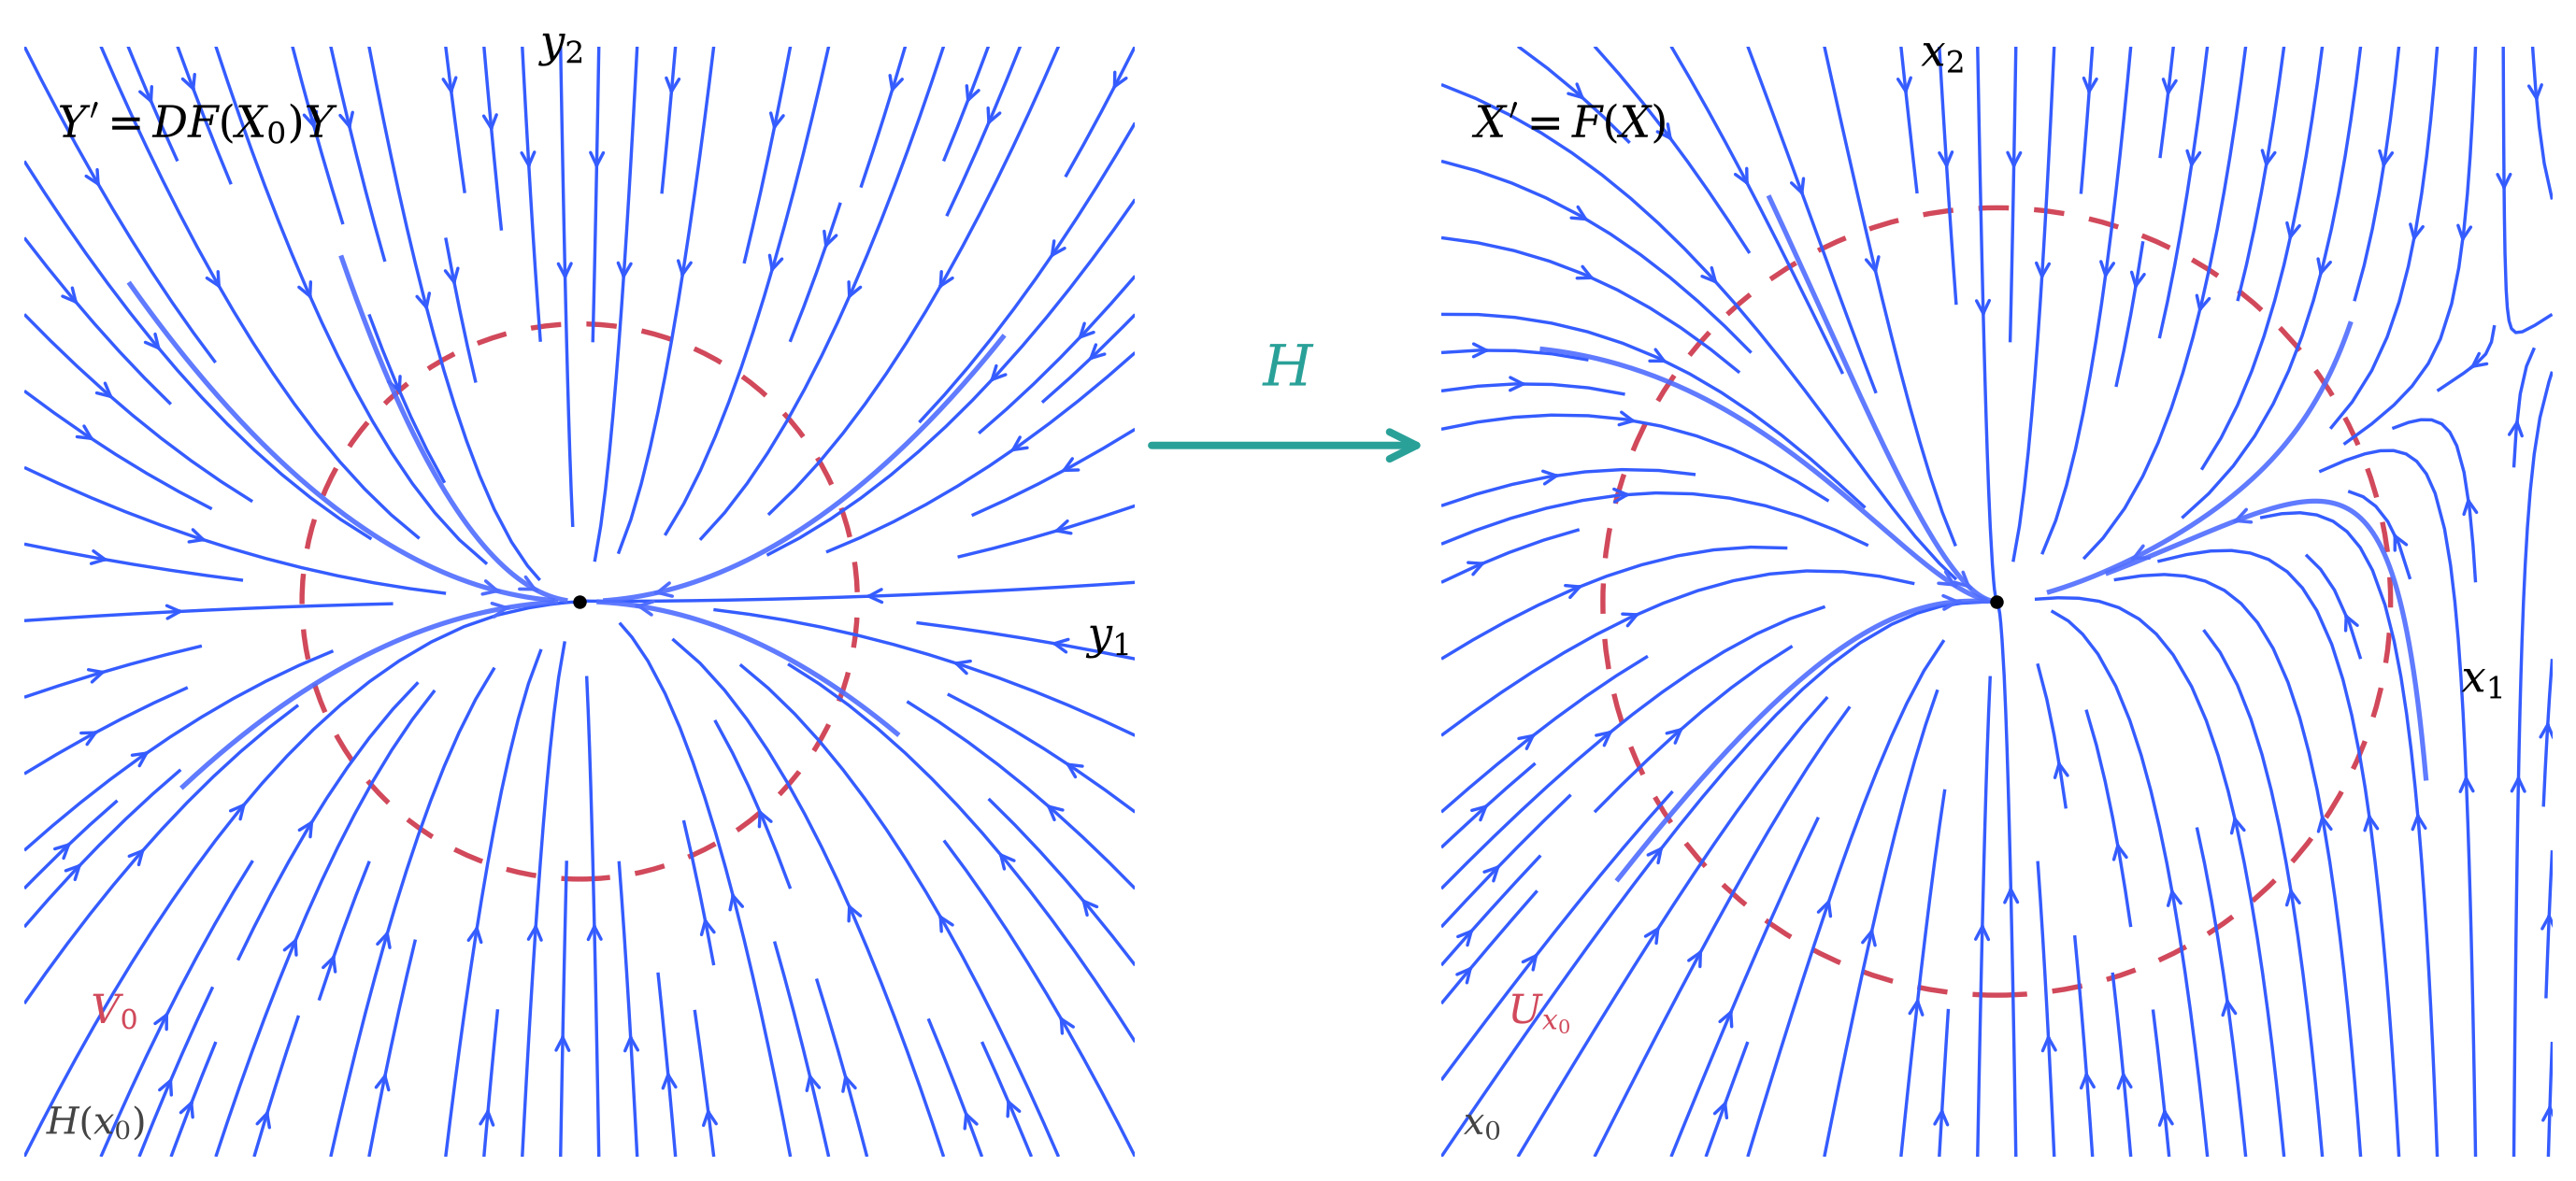
\includegraphics[width=0.98\linewidth]{fig_17_hg_conjugacion_local.png}
\caption{Retratos de fase locales: a la izquierda el sistema linealizado
$Y'=DF(X_0)Y$, a la derecha el sistema no lineal $X'=F(X)$, unidos por
la conjugación local $H$.}
\end{figure}

\subsection{Ejemplo trabajado: verificación de Hartman-Grobman}

Consideremos el sistema
\begin{align*}
x_1' &= -x_1 + x_1^2,\\
x_2' &= -2x_2 + x_1^2.
\end{align*}

\textbf{Puntos de equilibrio.} De $-x_1+x_1^2=x_1(x_1-1)=0$ obtenemos
$x_1=0$ o $x_1=1$. Para cada caso:
\[
x_1=0 \Rightarrow x_2=0 \quad (X_0=(0,0)),\qquad
x_1=1 \Rightarrow x_2=\tfrac{1}{2} \quad (X_1=(1,\tfrac{1}{2})).
\]

\textbf{Jacobiano:}
\[
J(X)=DF(X)=\begin{pmatrix}2x_1-1 & 0\\ 2x_1 & -2\end{pmatrix}.
\]

\textbf{Equilibrio $X_0=(0,0)$:}
\[
A=J(X_0)=\begin{pmatrix}-1 & 0\\ 0 & -2\end{pmatrix},\qquad
p(\lambda)=(\lambda+1)(\lambda+2),\quad \lambda_1=-1,\;\lambda_2=-2.
\]
Ambos valores propios son reales negativos, así que $X_0$ es un \textbf{sumidero}
(nodo estable). Como ningún valor propio tiene parte real nula, $X_0$ es
hiperbólico y H-G garantiza que el no lineal también tiene un sumidero en $X_0$.

Los vectores propios son $V_1=\binom{1}{0}$ (para $\lambda_1=-1$)
y $V_2=\binom{0}{1}$ (para $\lambda_2=-2$), y la solución general del sistema
linealizado es
\[
Y(t)=c_1 e^{-t}\binom{1}{0}+c_2 e^{-2t}\binom{0}{1}.
\]

\textbf{Equilibrio $X_1=(1,\frac{1}{2})$:}
\[
J(X_1)=\begin{pmatrix}1 & 0\\ 2 & -2\end{pmatrix},\qquad
p(\lambda)=(1-\lambda)(-2-\lambda),\quad \lambda_1=1,\;\lambda_2=-2.
\]
Los valores propios tienen signos opuestos: $X_1$ es una \textbf{silla hiperbólica}.
La solución del sistema linealizado en variables locales $Y=X-X_1$ es:
\[
Y(t)=c_1 e^{t}\binom{3}{2}+c_2 e^{-2t}\binom{0}{1}.
\]
Por Hartman-Grobman, el sistema no lineal cerca de $X_1$ es topológicamente
conjugado a esta silla lineal: las soluciones se acercan sobre la variedad
estable y se alejan por la variedad inestable.

\begin{figure}[H]
\centering
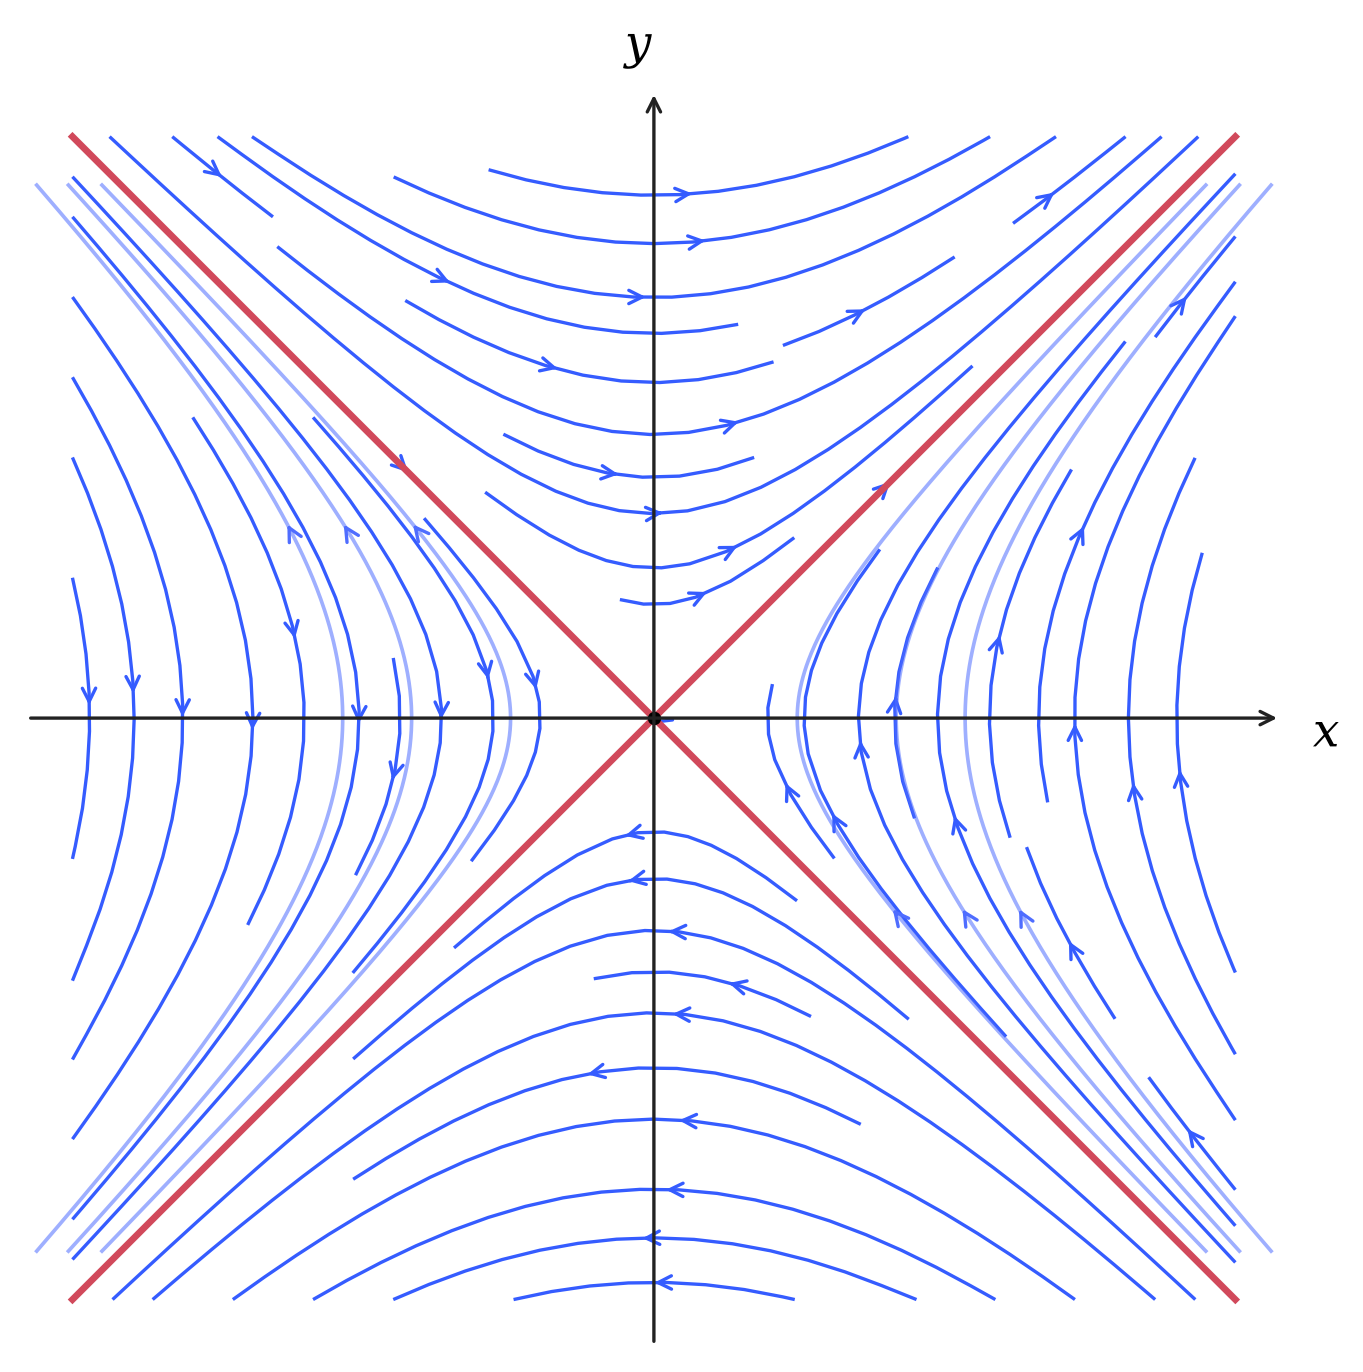
\includegraphics[width=0.94\linewidth]{fig_14_flujo_silla.png}
\caption{Retrato de fase tipo silla con separatrices y trayectorias. Las flechas
rojas indican la variedad inestable (crecimiento exponencial) y las azules la
variedad estable (decaimiento exponencial).}
\end{figure}

\subsection{Limitación de Hartman-Grobman: el no-ejemplo}

Cuando el equilibrio \textbf{no es hiperbólico}, el teorema H-G no aplica y
el comportamiento del sistema no lineal puede diferir cualitativamente del lineal.

Considérese el sistema
\begin{align*}
x' &= -y + x(x^2+y^2),\\
y' &= x + y(x^2+y^2).
\end{align*}
El origen es el único equilibrio. El jacobiano en $(0,0)$ es
\[
DF(0,0)=\begin{pmatrix}0 & -1\\ 1 & 0\end{pmatrix},\qquad p(\lambda)=\lambda^2+1,\quad \lambda=\pm i.
\]
Como los valores propios son puramente imaginarios, el origen \textbf{no es hiperbólico}.
El sistema linealizado tiene un \textbf{centro}: las soluciones son
circunferencias periódicas de período $2\pi$.

Sin embargo, pasando a coordenadas polares $r^2=x^2+y^2$, se verifica que
\[
\dot{r}=\frac{x\dot{x}+y\dot{y}}{r}=r^3,\qquad \dot{\theta}=1.
\]
Por lo tanto, el radio \emph{crece} con el tiempo (las órbitas son espirales
salientes), lo que es cualitativamente distinto al centro. La diferencia no es
topológicamente equivalente: H-G no aplica.

\begin{figure}[H]
\centering
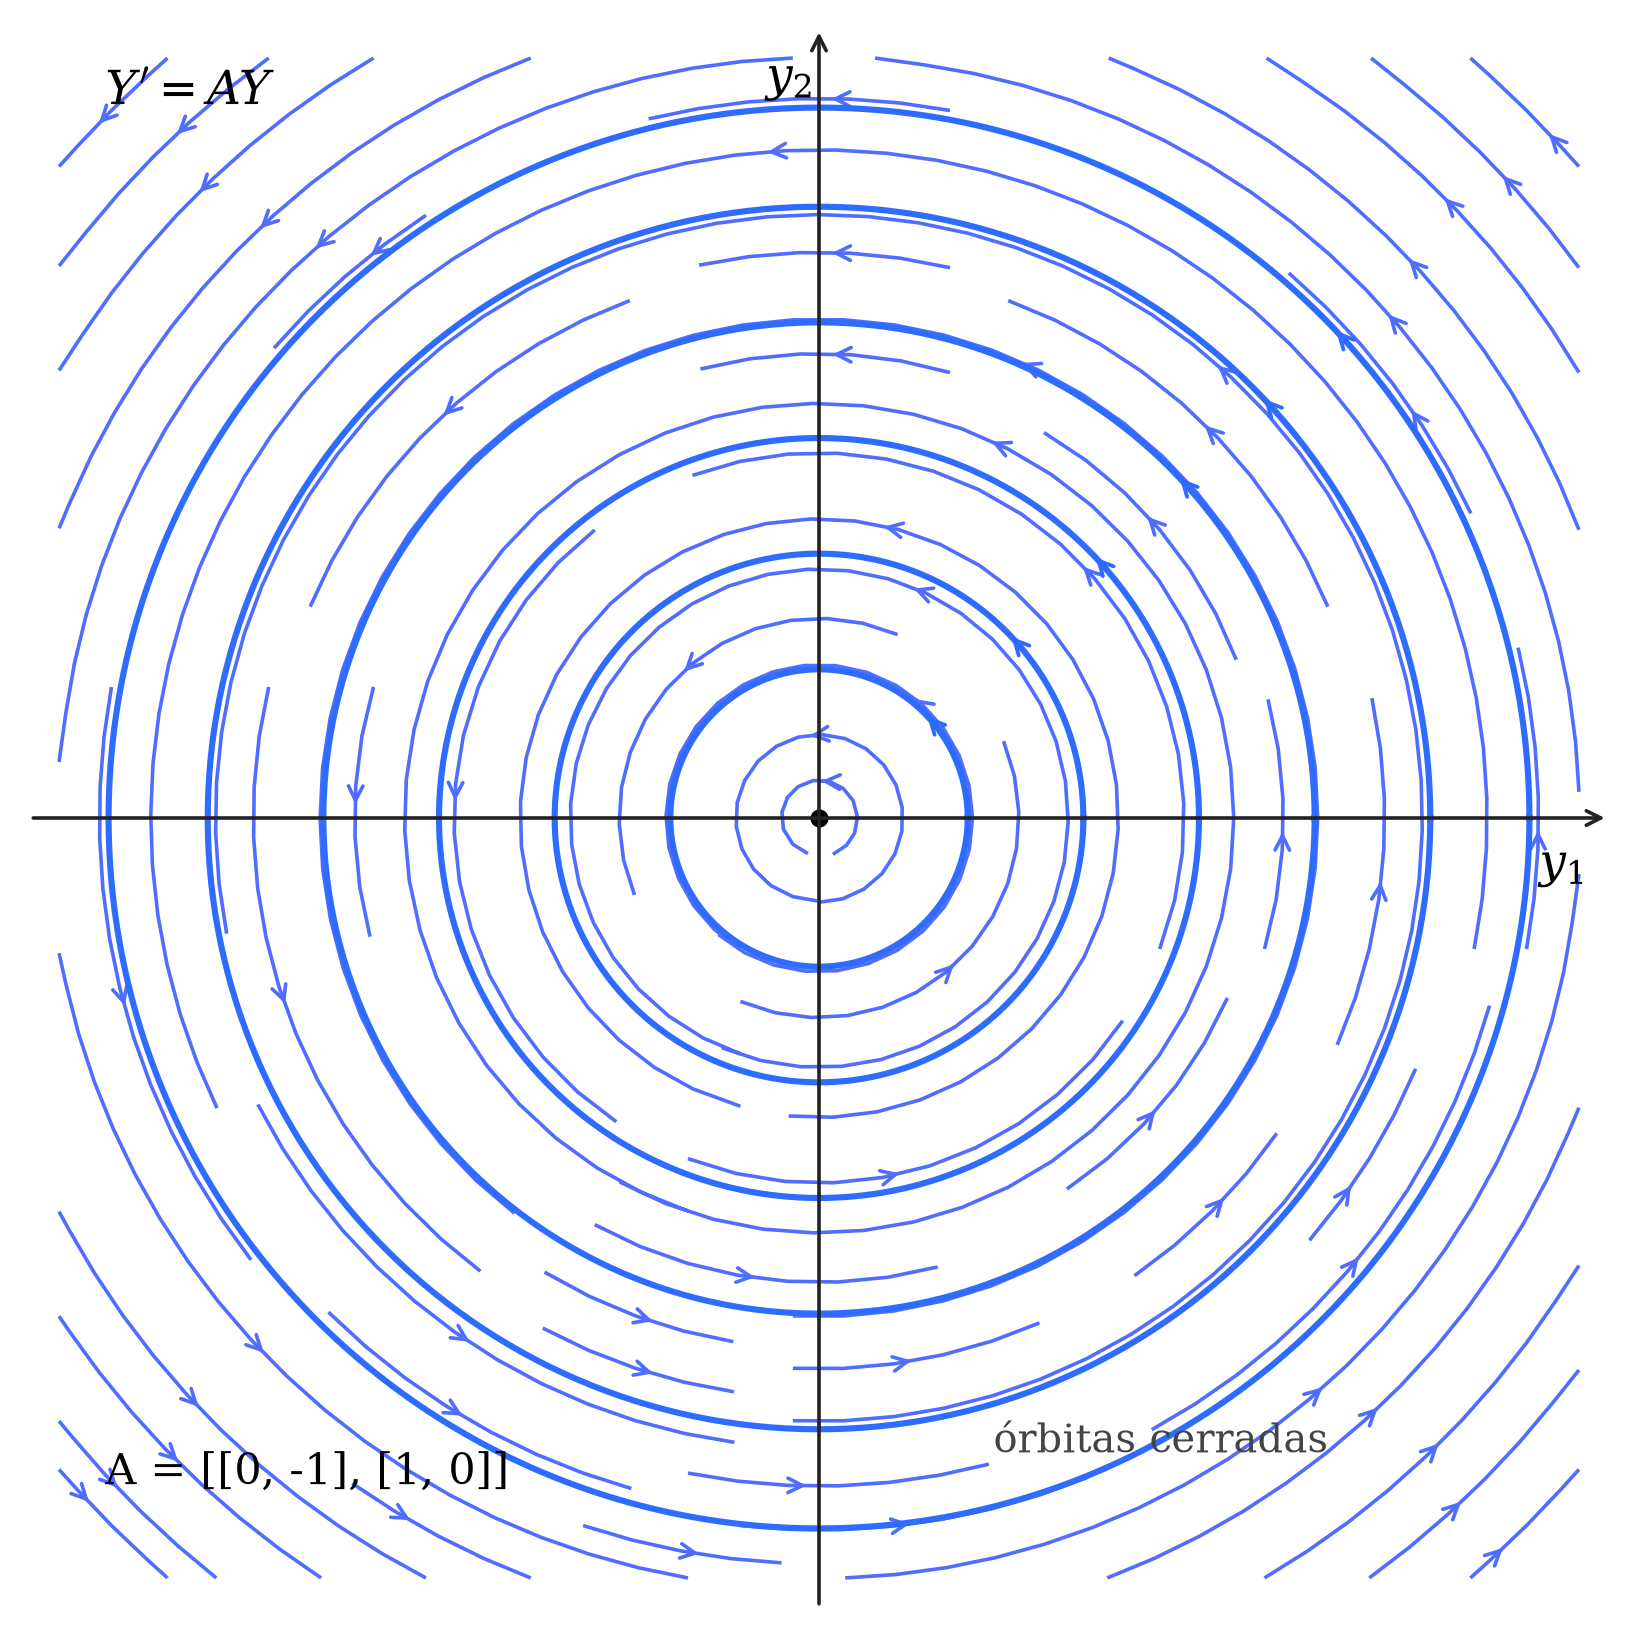
\includegraphics[width=0.94\linewidth]{fig_18_sistema_lineal_periodico.png}
\caption{Sistema linealizado $Y'=AY$: trayectorias cerradas (centro en el origen).}
\end{figure}

\begin{figure}[H]
\centering
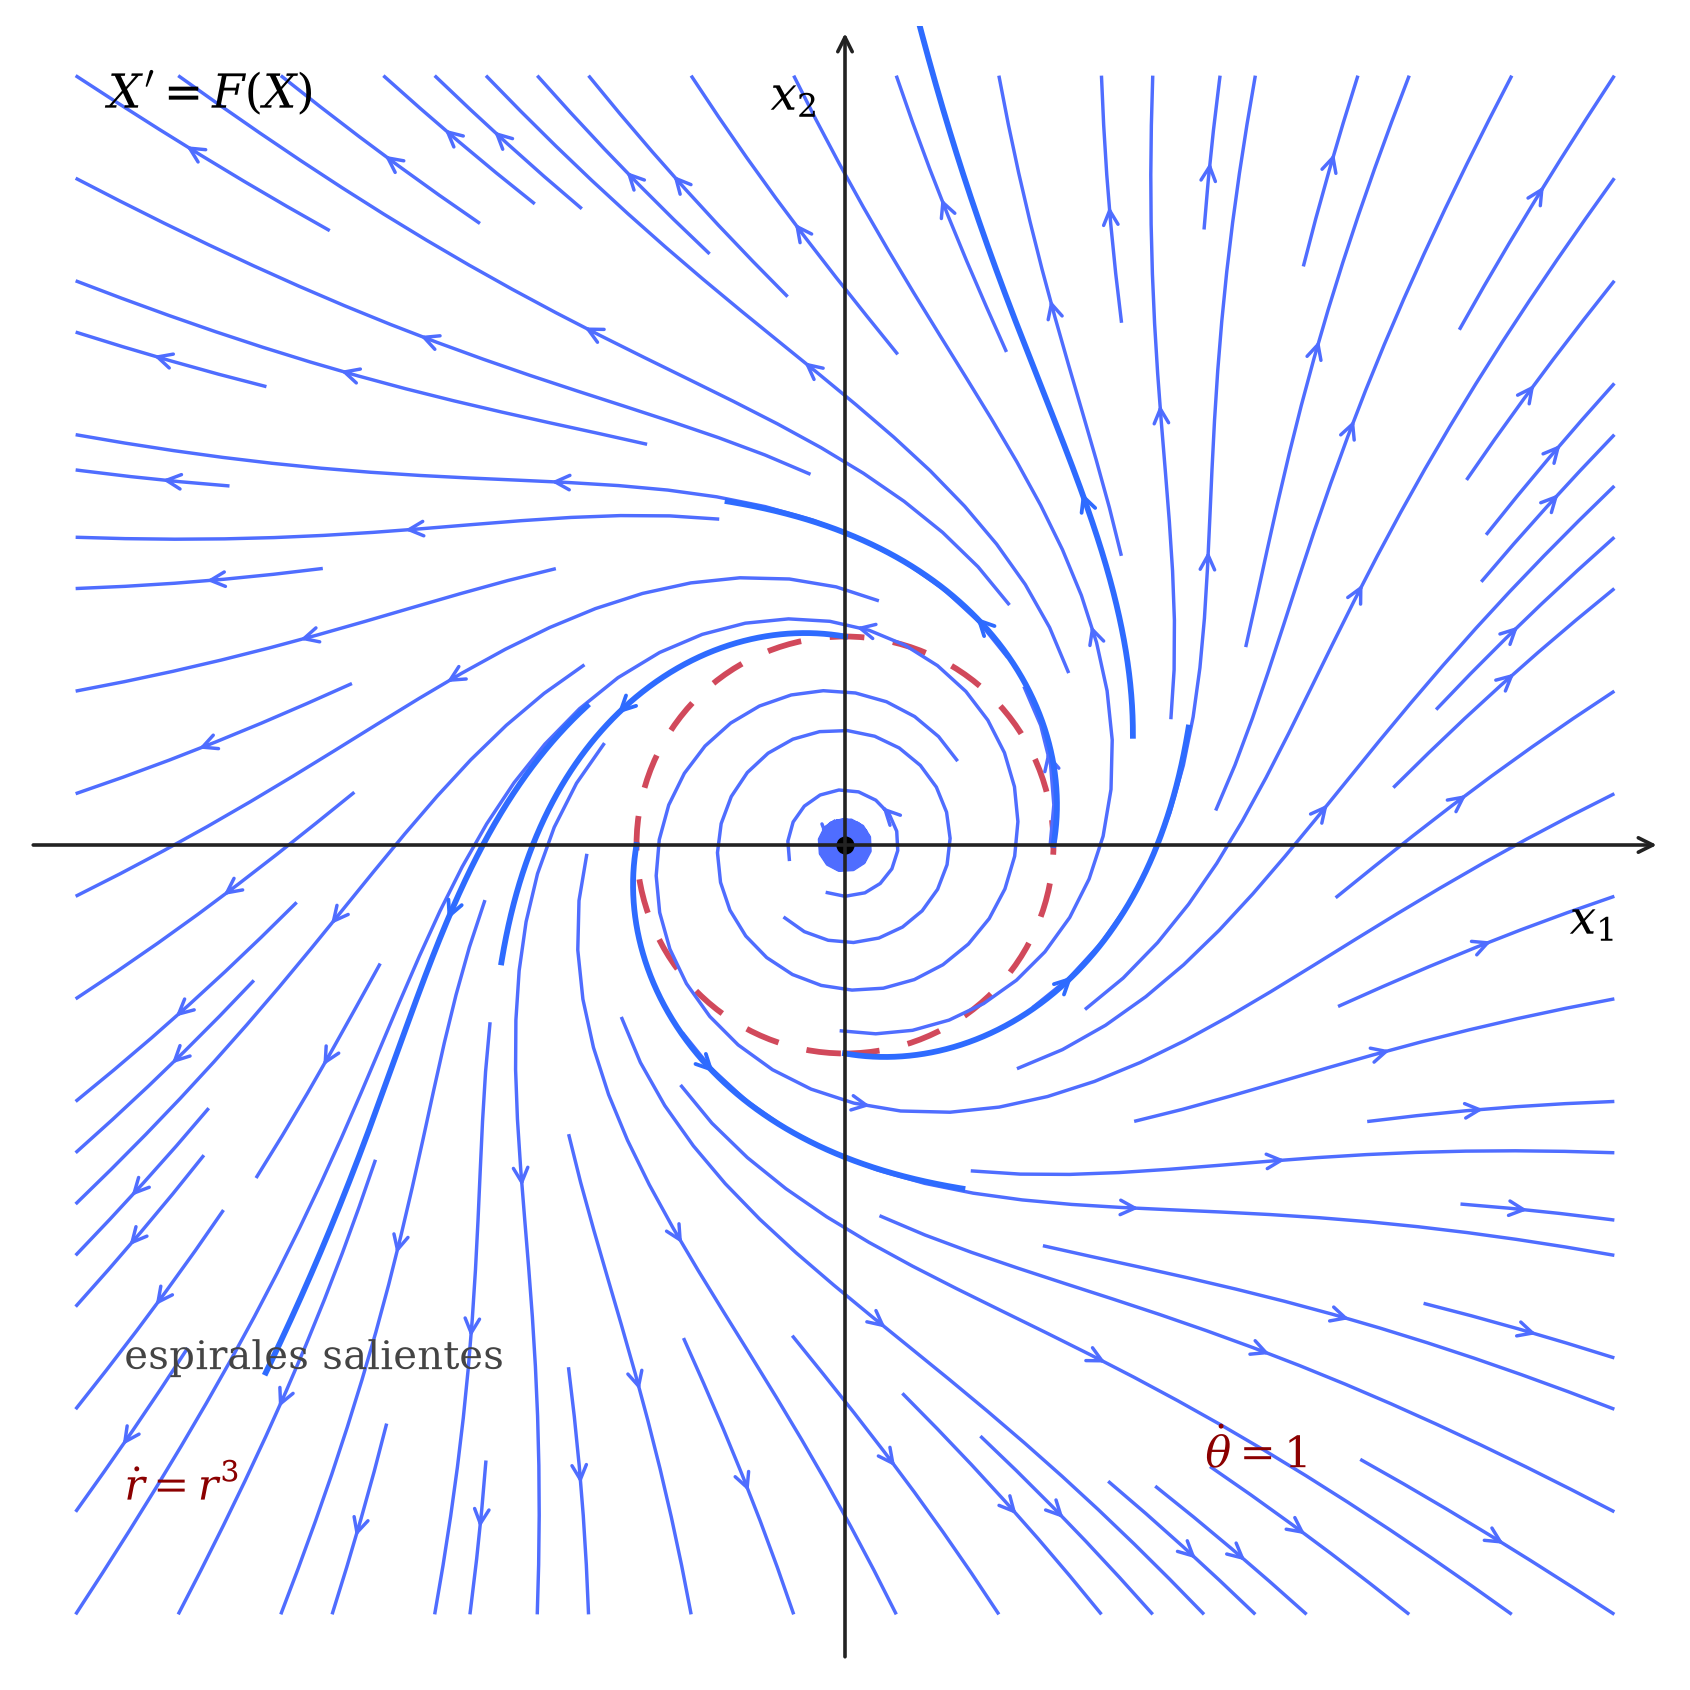
\includegraphics[width=0.94\linewidth]{fig_19_no_ejemplo_espiral.png}
\caption{Sistema no lineal: las trayectorias son espirales salientes, coherentes
con $\dot{r}=r^3$. El comportamiento cualitativo difiere del linealizado.}
\end{figure}

% ============================================================
\section{Flujo de un sistema dinámico y conjugación topológica}
\label{sec:flujo-conjugacion}
% ============================================================

\subsection{El flujo asociado a un sistema}

Dado un sistema $x'=F(x)$ en $\mathbb{R}^n$ de clase $C^1$, para cada condición
inicial $x\in\mathbb{R}^n$ existe una solución única $x(t)$. Esto define una
familia de aplicaciones indexadas por el tiempo:

\begin{definicion}{Flujo}{}
El \textbf{flujo} asociado a $x'=F(x)$ es la aplicación
\[
\varphi:\mathbb{R}\times\mathbb{R}^n\to\mathbb{R}^n,\qquad (t,x)\mapsto\varphi(t,x)=\varphi_t(x),
\]
donde $\varphi_t(x)$ es la solución en el tiempo $t$ con condición inicial $x$.
\end{definicion}

El flujo satisface tres propiedades fundamentales:
\begin{enumerate}
    \item \textbf{Identidad inicial:} $\varphi_0(x)=x$ (la solución en $t=0$ es la condición inicial).
    \item \textbf{Propiedad de grupo (composición):} $\varphi_s(\varphi_t(x))=\varphi_{s+t}(x)$
          (evolucionar $t$ unidades y luego $s$ unidades es lo mismo que evolucionar $s+t$).
    \item \textbf{Ecuación del flujo:} $\dfrac{d}{dt}\varphi_t(x)=F(\varphi_t(x))$.
\end{enumerate}

\textbf{Verificación para $x'=ax$:} la solución es $\varphi_t(x)=xe^{at}$.
\begin{align*}
\varphi_0(x) &= xe^0 = x \checkmark\\
\varphi_s(\varphi_t(x)) &= \varphi_s(xe^{at}) = xe^{at}e^{as} = xe^{a(s+t)} = \varphi_{s+t}(x)\checkmark
\end{align*}

\begin{figure}[H]
\centering
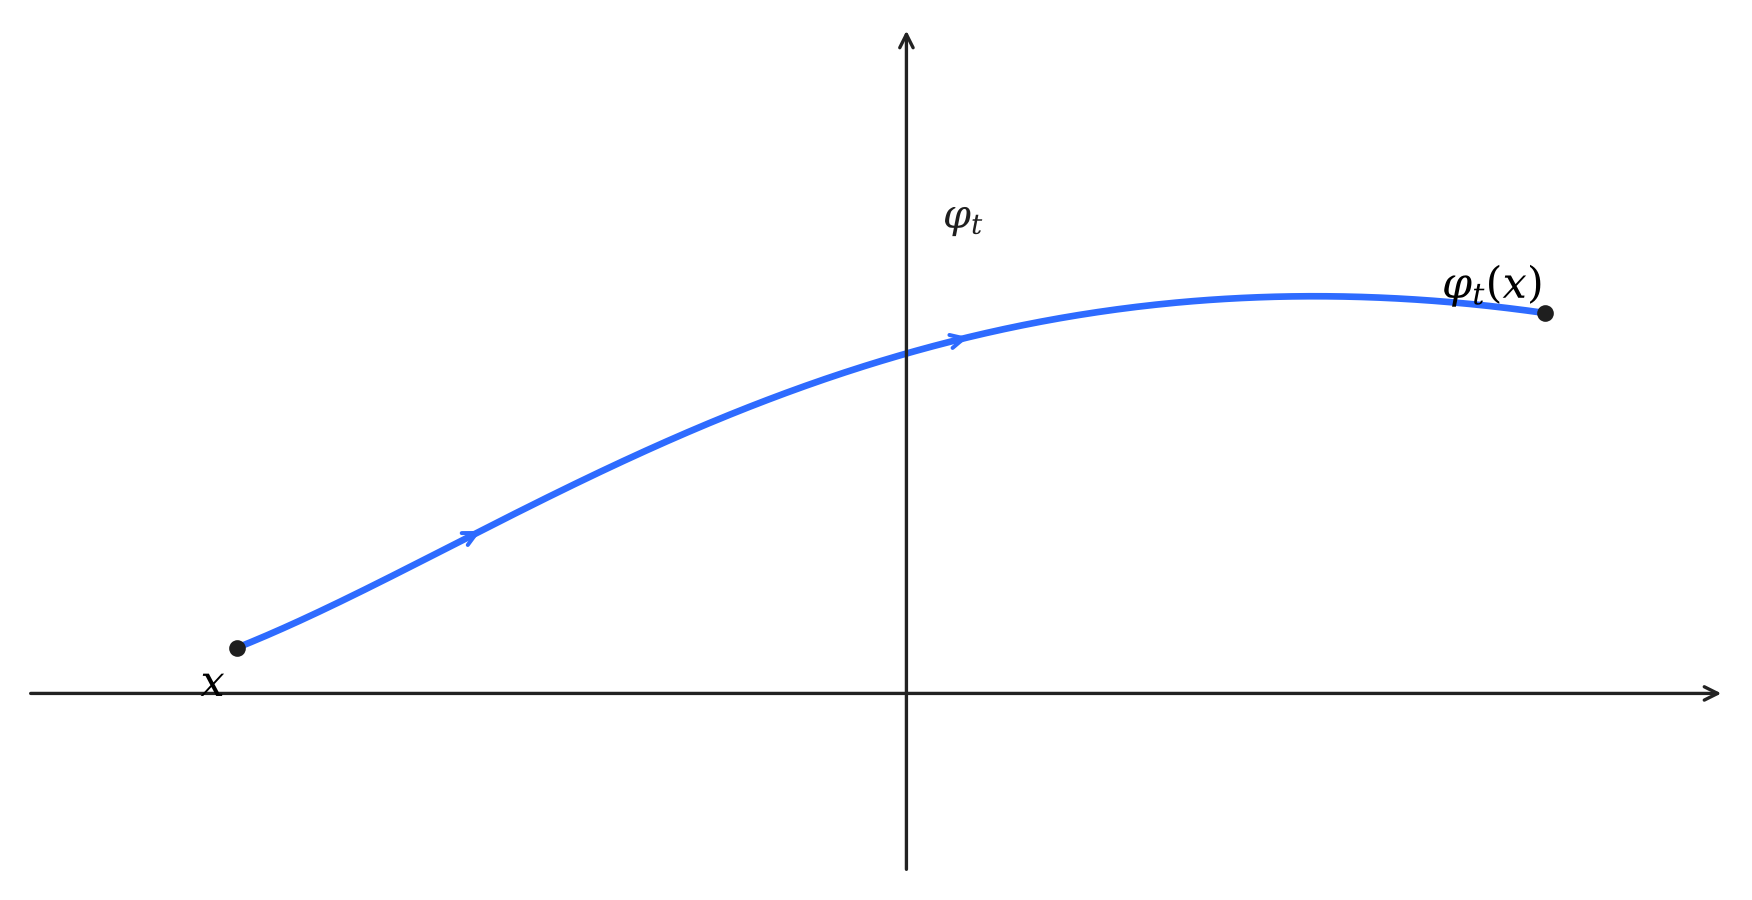
\includegraphics[width=0.96\linewidth]{fig_15_flujo_orbita.png}
\caption{Trayectoria de una solución bajo el flujo $\varphi_t$: la condición inicial
$x$ se transporta a lo largo de la curva integral.}
\end{figure}

\begin{figure}[H]
\centering
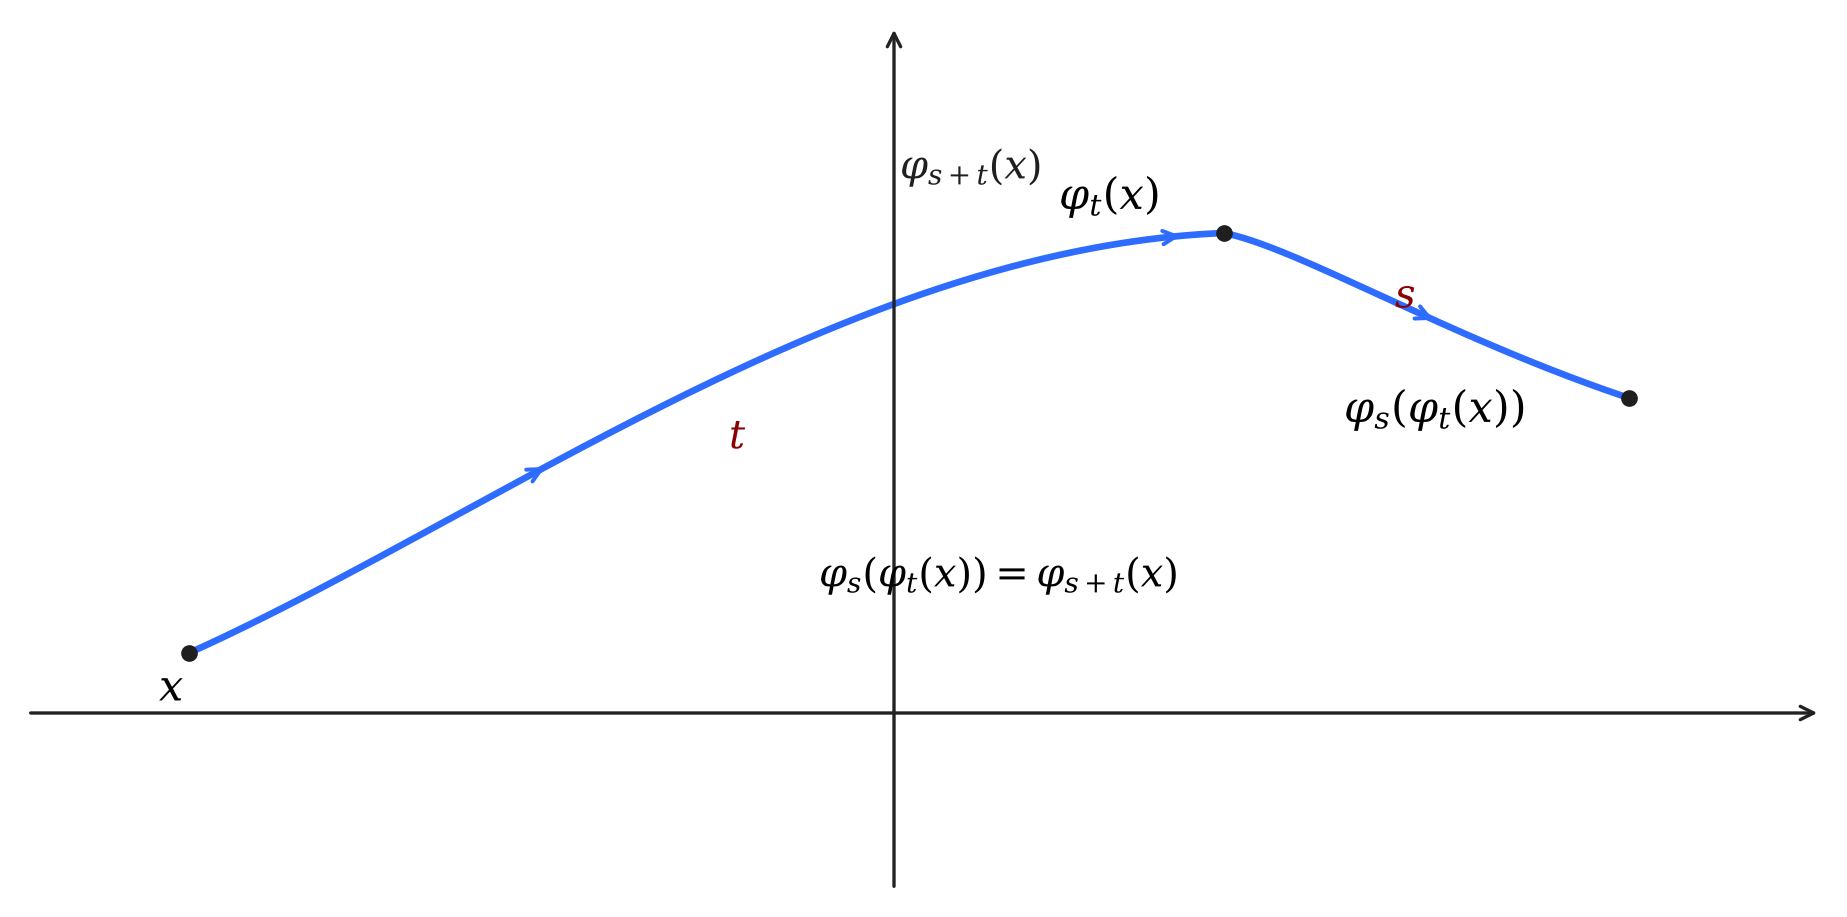
\includegraphics[width=0.96\linewidth]{fig_16_flujo_composicion.png}
\caption{Propiedad de composición $\varphi_s(\varphi_t(x))=\varphi_{s+t}(x)$:
las evoluciones sucesivas son equivalentes a una única evolución de duración $s+t$.}
\end{figure}

\subsection{Conjugación topológica}

La conjugación topológica es la noción precisa que formaliza cuándo dos sistemas
dinámicos son ``cualitativamente equivalentes'': sus flujos se relacionan mediante
un cambio de coordenadas continuo e invertible.

\begin{definicion}{Conjugación topológica local}{}
Sean $x'=F(x)$ e $y'=G(y)$ dos sistemas de clase $C^1$, con $x_0$ e $y_0$
puntos de equilibrio respectivos y flujos $\varphi_t$, $\psi_t$.
Decimos que son \textbf{localmente topológicamente conjugados} alrededor de
$x_0$ e $y_0$ si existen:
\begin{itemize}
    \item Vecindades $U_{x_0}$ y $V_{y_0}$,
    \item Un homeomorfismo $H:U_{x_0}\to V_{y_0}$
\end{itemize}
tal que $H(\varphi_t(x))=\psi_t(H(x))$ para todo $x\in U_{x_0}$ y $t$ suficientemente pequeño.
\end{definicion}

La conjugación topológica preserva la estructura cualitativa del flujo: órbitas
en órbitas, equilibrios en equilibrios, y el sentido de recorrido. No preserva
necesariamente distancias ni tiempos.

% ============================================================
\section{Isoclinas nulas y análisis cualitativo en el plano}
\label{sec:isoclinas}
% ============================================================

Para un sistema $X'=F(X)$ con $F=(f,g)$ en $\mathbb{R}^2$, las
\textbf{isoclinas nulas} (nullclines) son las curvas donde cada componente
del campo se anula:
\[
I_1:\; f(x,y)=0 \quad(\text{isoclina de }x'),\qquad
I_2:\; g(x,y)=0 \quad(\text{isoclina de }y').
\]
En $I_1$ el campo es vertical: $F=\binom{0}{g(x,y)}$.
En $I_2$ el campo es horizontal: $F=\binom{f(x,y)}{0}$.
Las isoclinas dividen el plano en regiones donde el signo de cada componente
es constante, permitiendo esbozar el campo sin integrar.

\begin{figure}[H]
\centering
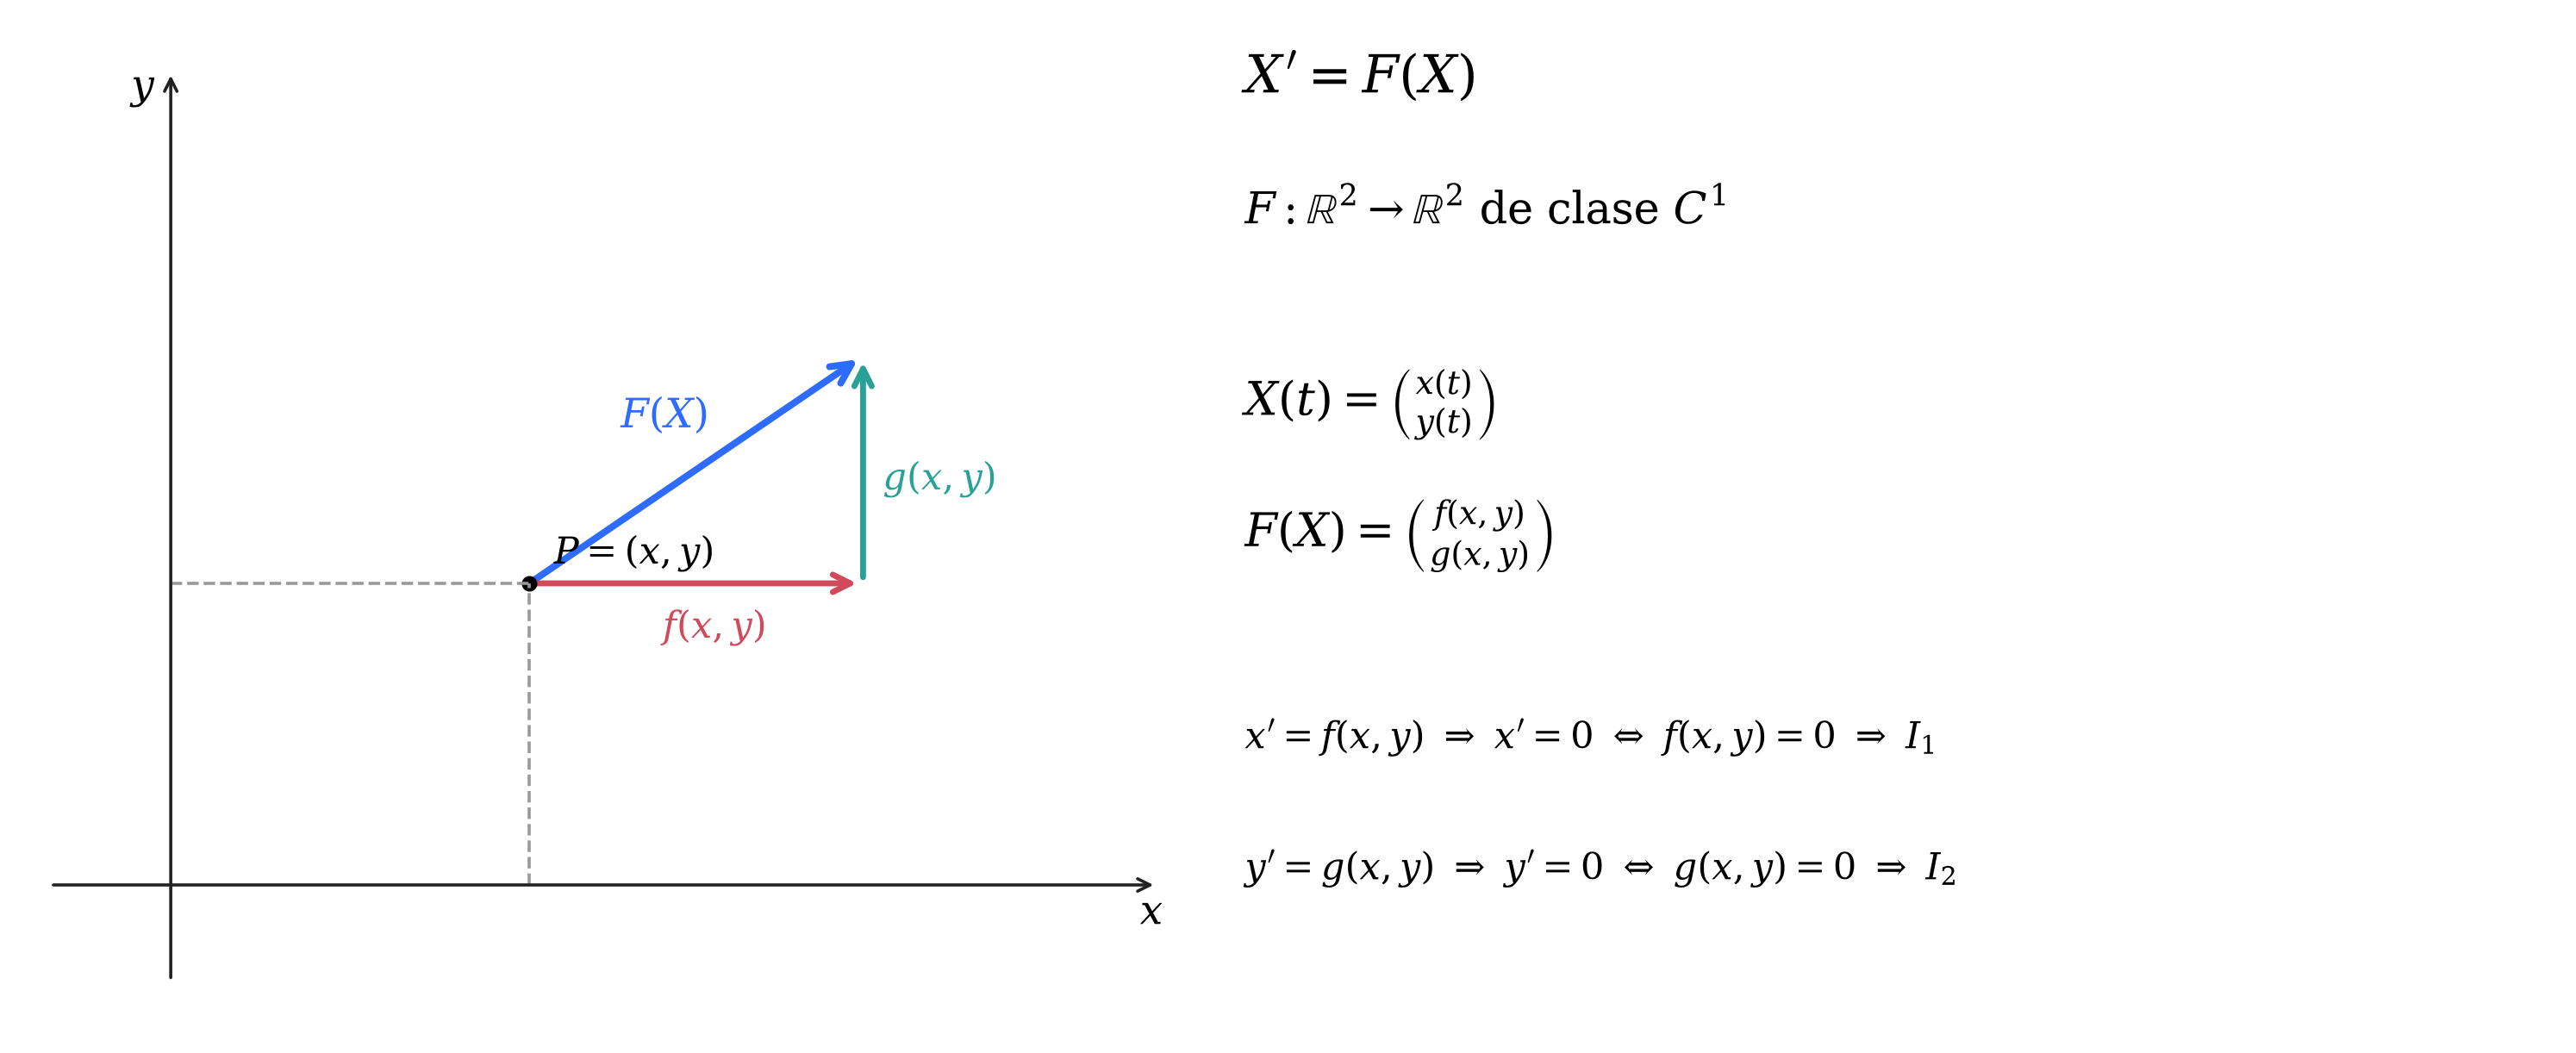
\includegraphics[width=0.92\linewidth]{fig_20_isoclinas_esquema.png}
\end{figure}

\begin{figure}[H]
\centering
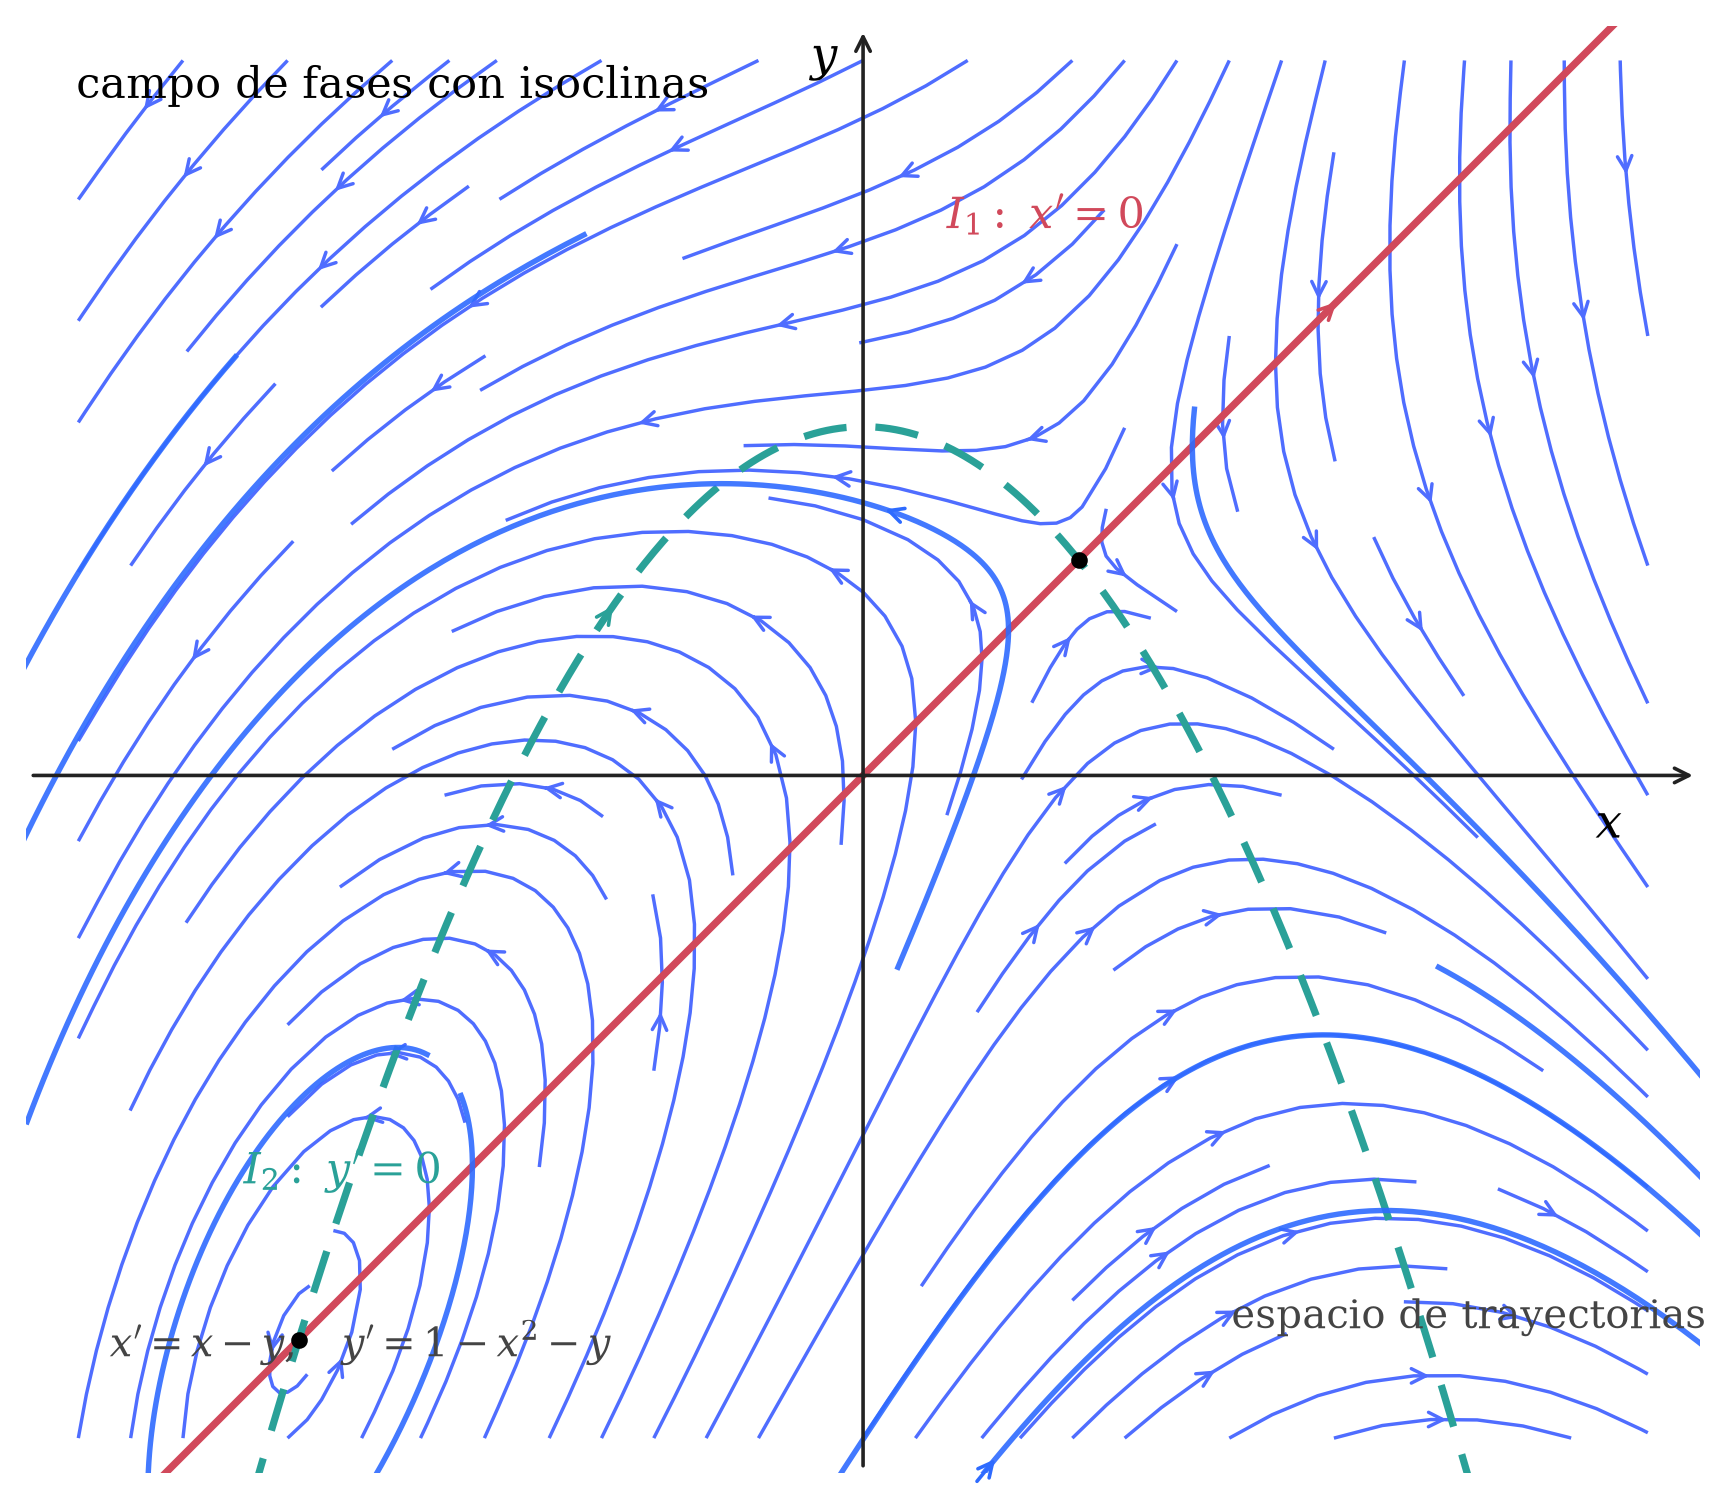
\includegraphics[width=0.92\linewidth]{fig_21_isoclinas_retrato.png}
\end{figure}

\begin{figure}[H]
\centering
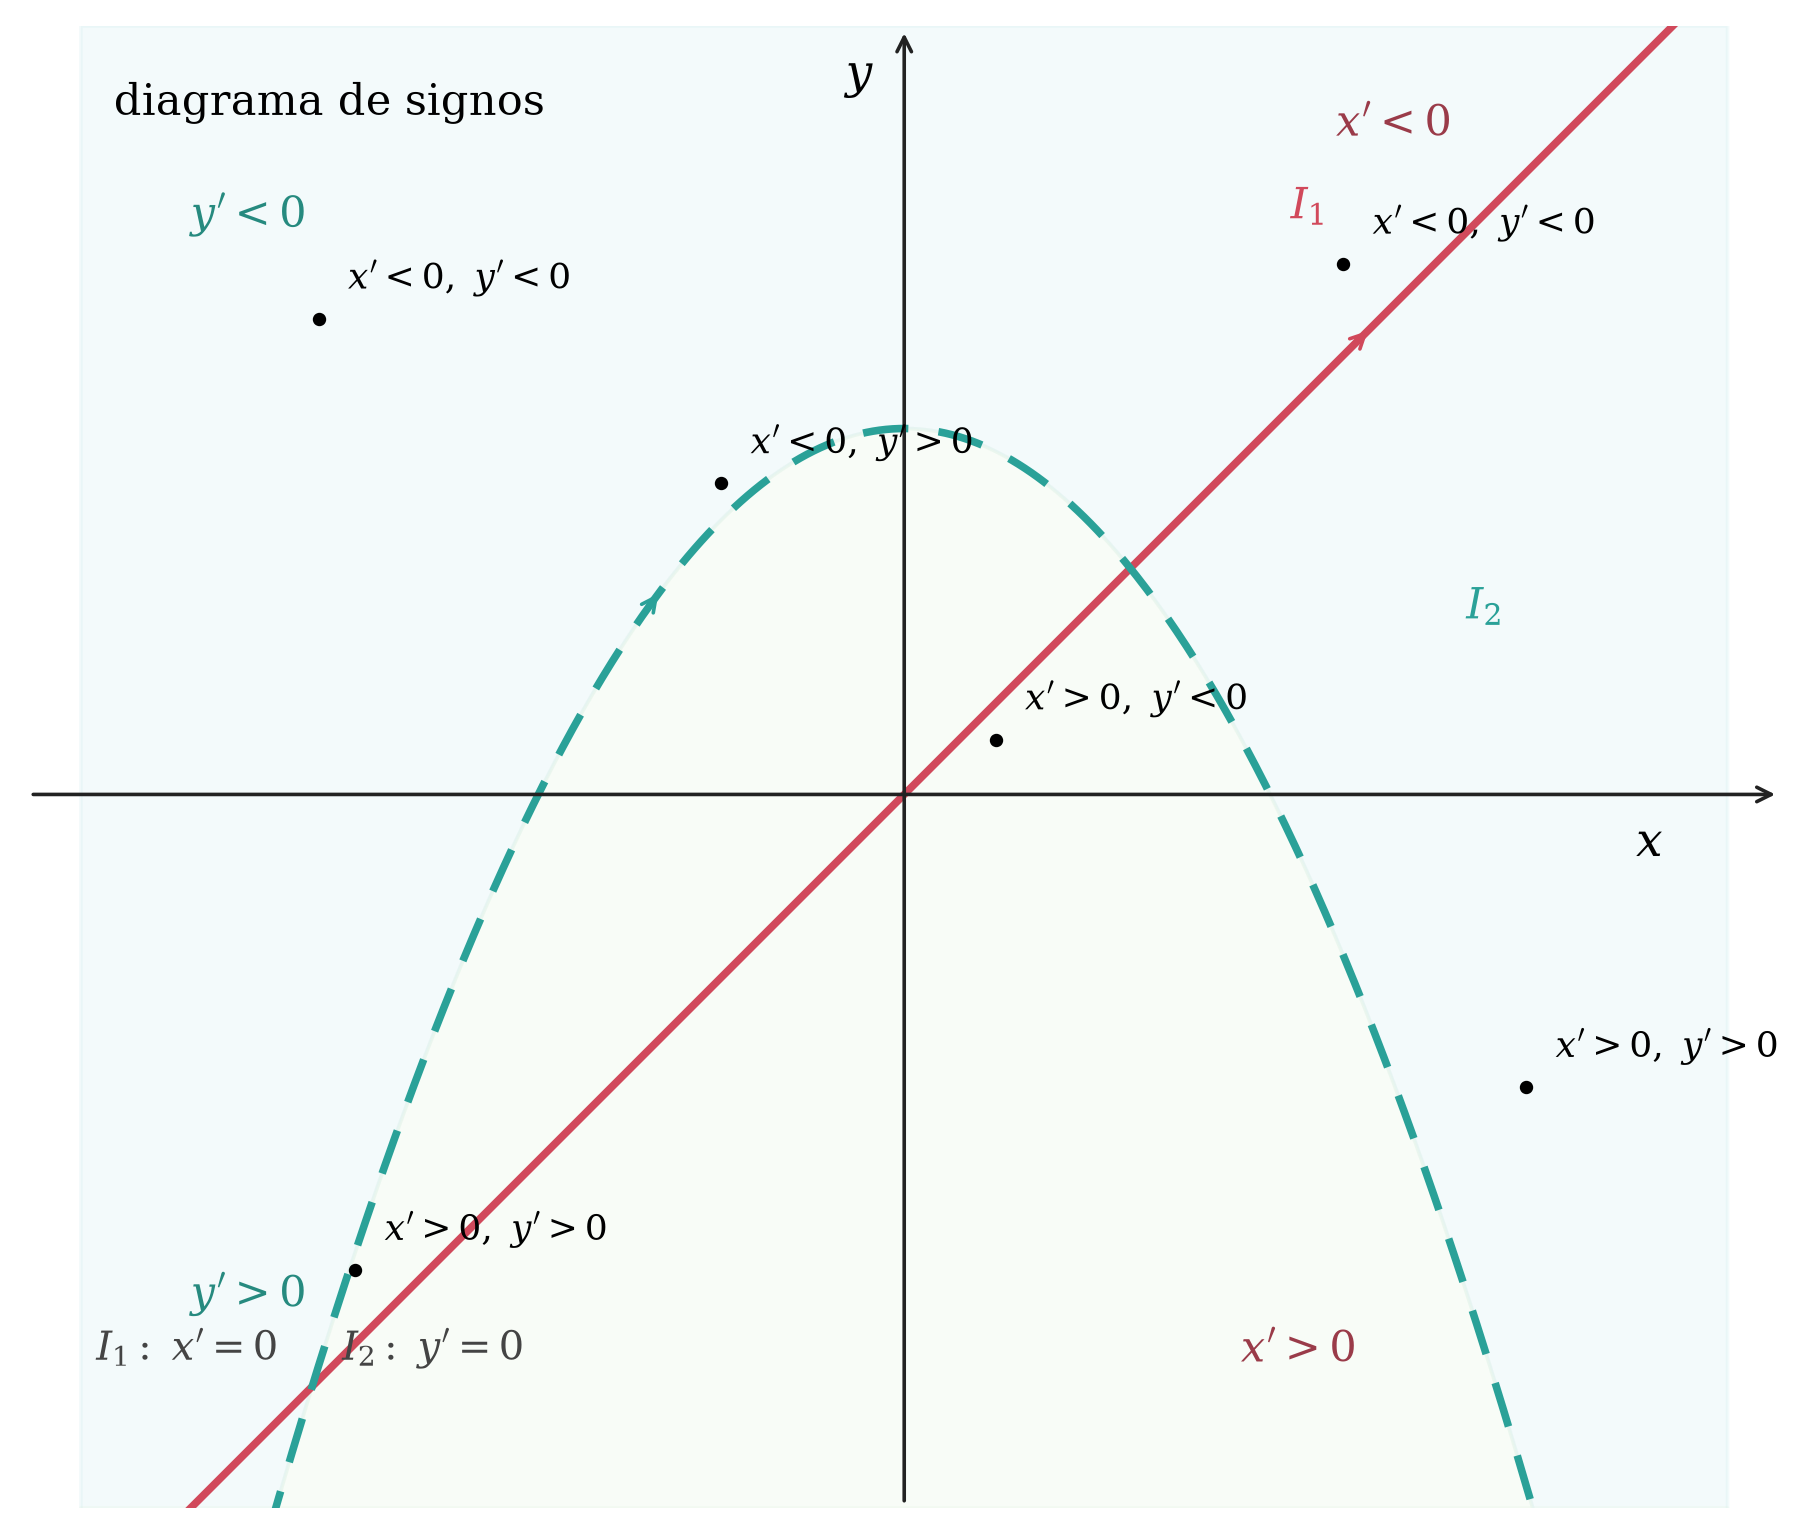
\includegraphics[width=0.92\linewidth]{fig_22_isoclinas_signos.png}
\end{figure}

\textbf{Ejemplo:} Sistema $x'=x(1-x-y)$, $y'=y(1-x)$.

Las isoclinas nulas son:
\begin{itemize}
    \item Para $x'$: $x=0$ o $y=1-x$.
    \item Para $y'$: $y=0$ o $x=1$.
\end{itemize}
Los ejes coordenados positivos son invariantes (si la población empieza en cero
no puede volverse negativa). Las isoclinas dividen el primer cuadrante en regiones
donde se lee el signo del campo directamente.

\begin{figure}[H]
\centering
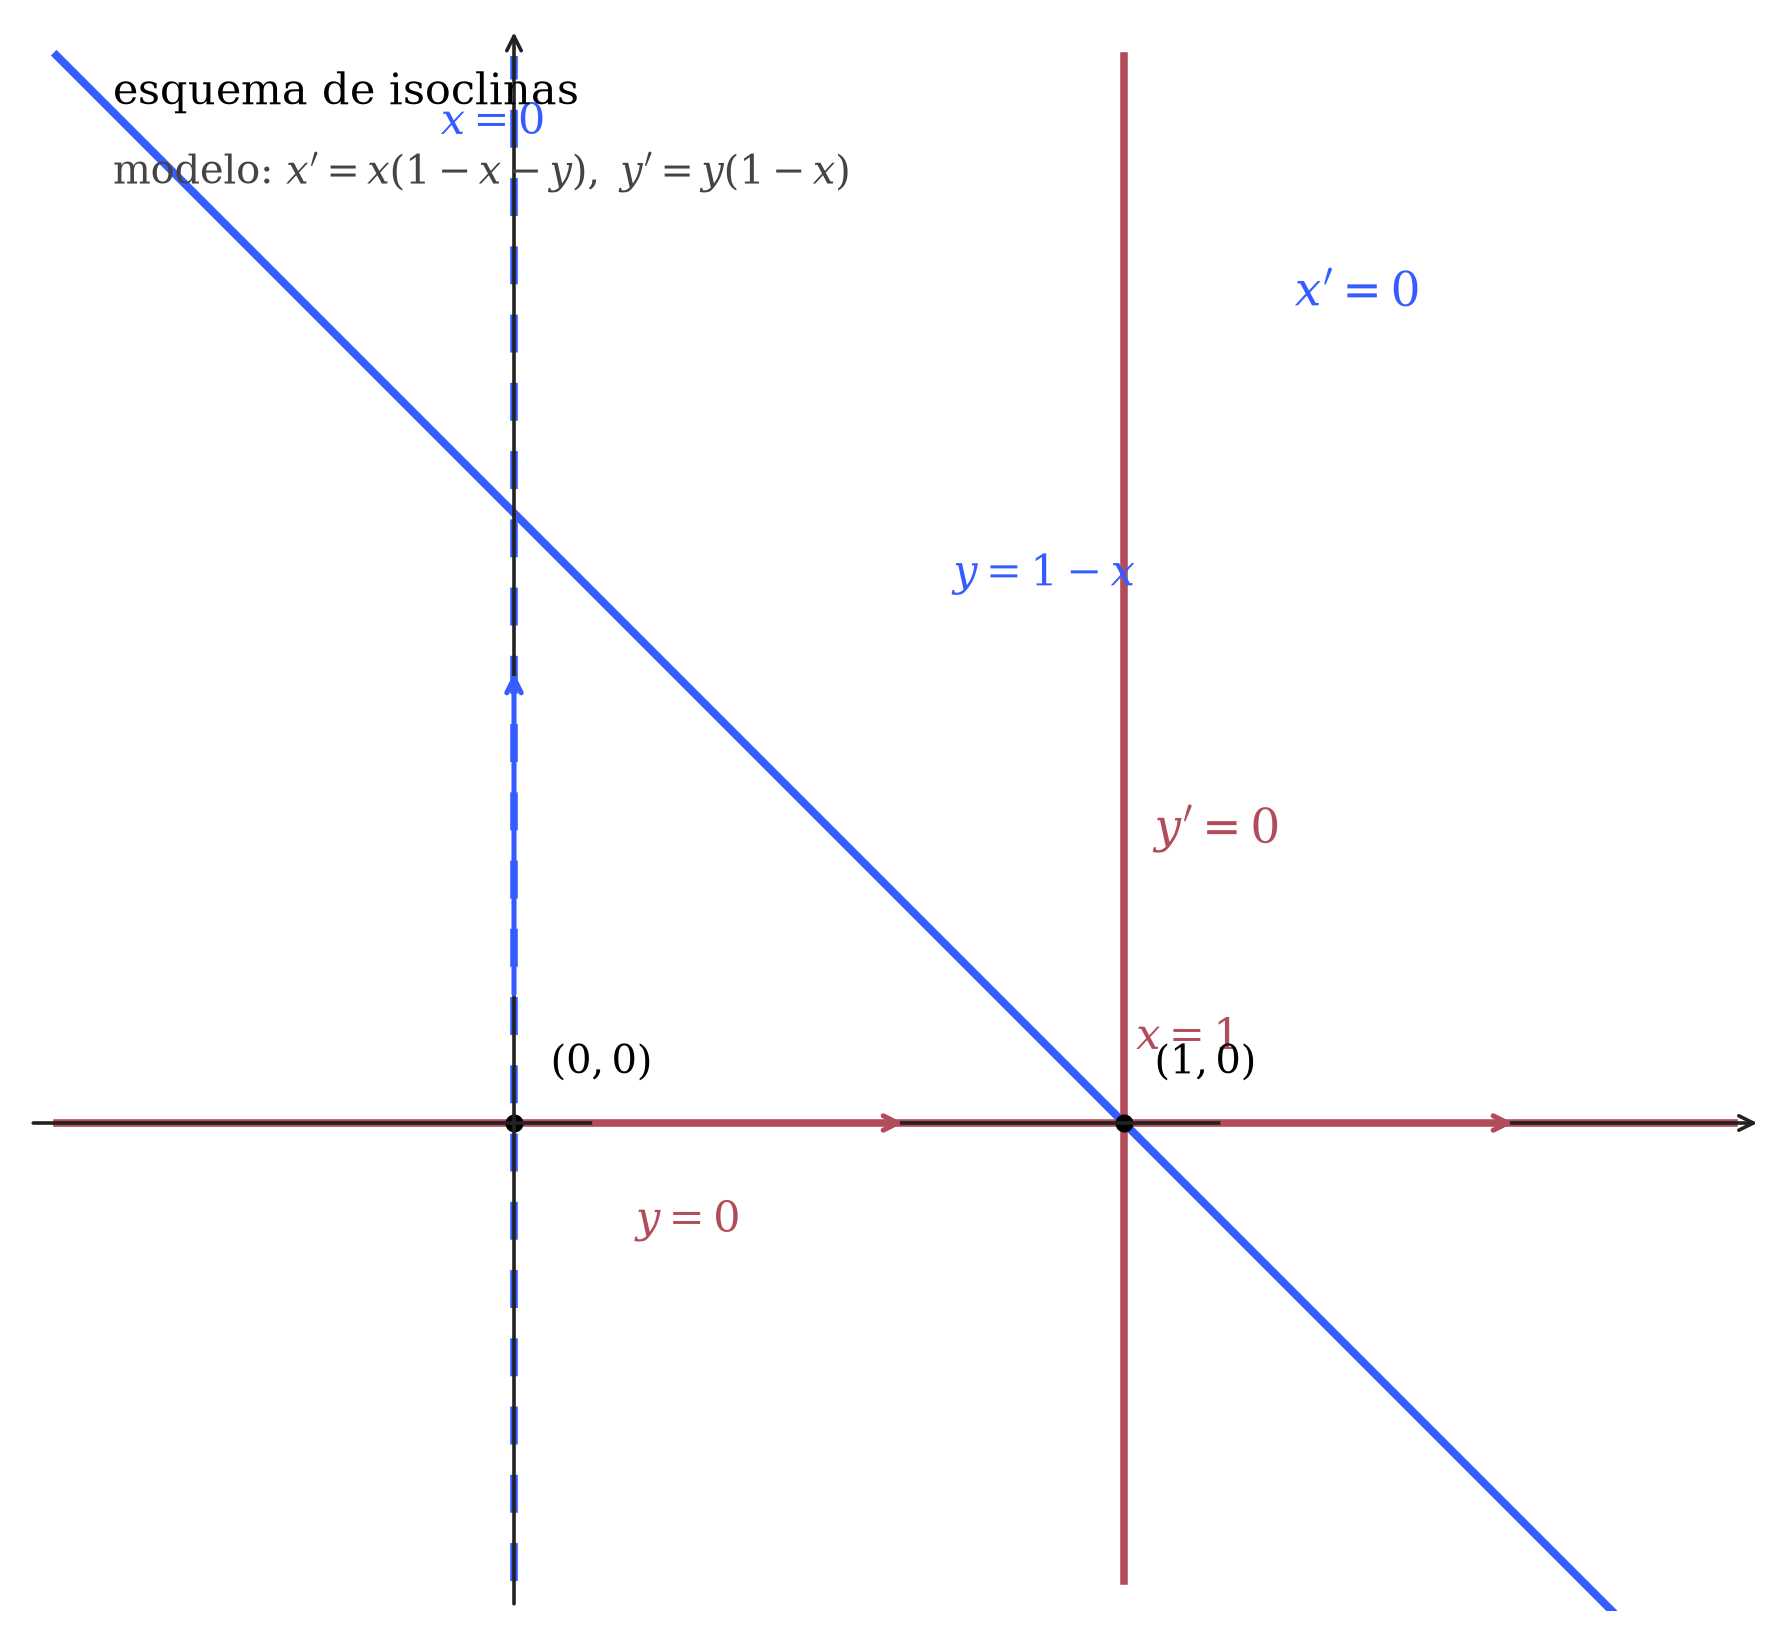
\includegraphics[width=0.92\linewidth]{fig_23_competencia_isoclinas.png}
\end{figure}

\begin{figure}[H]
\centering
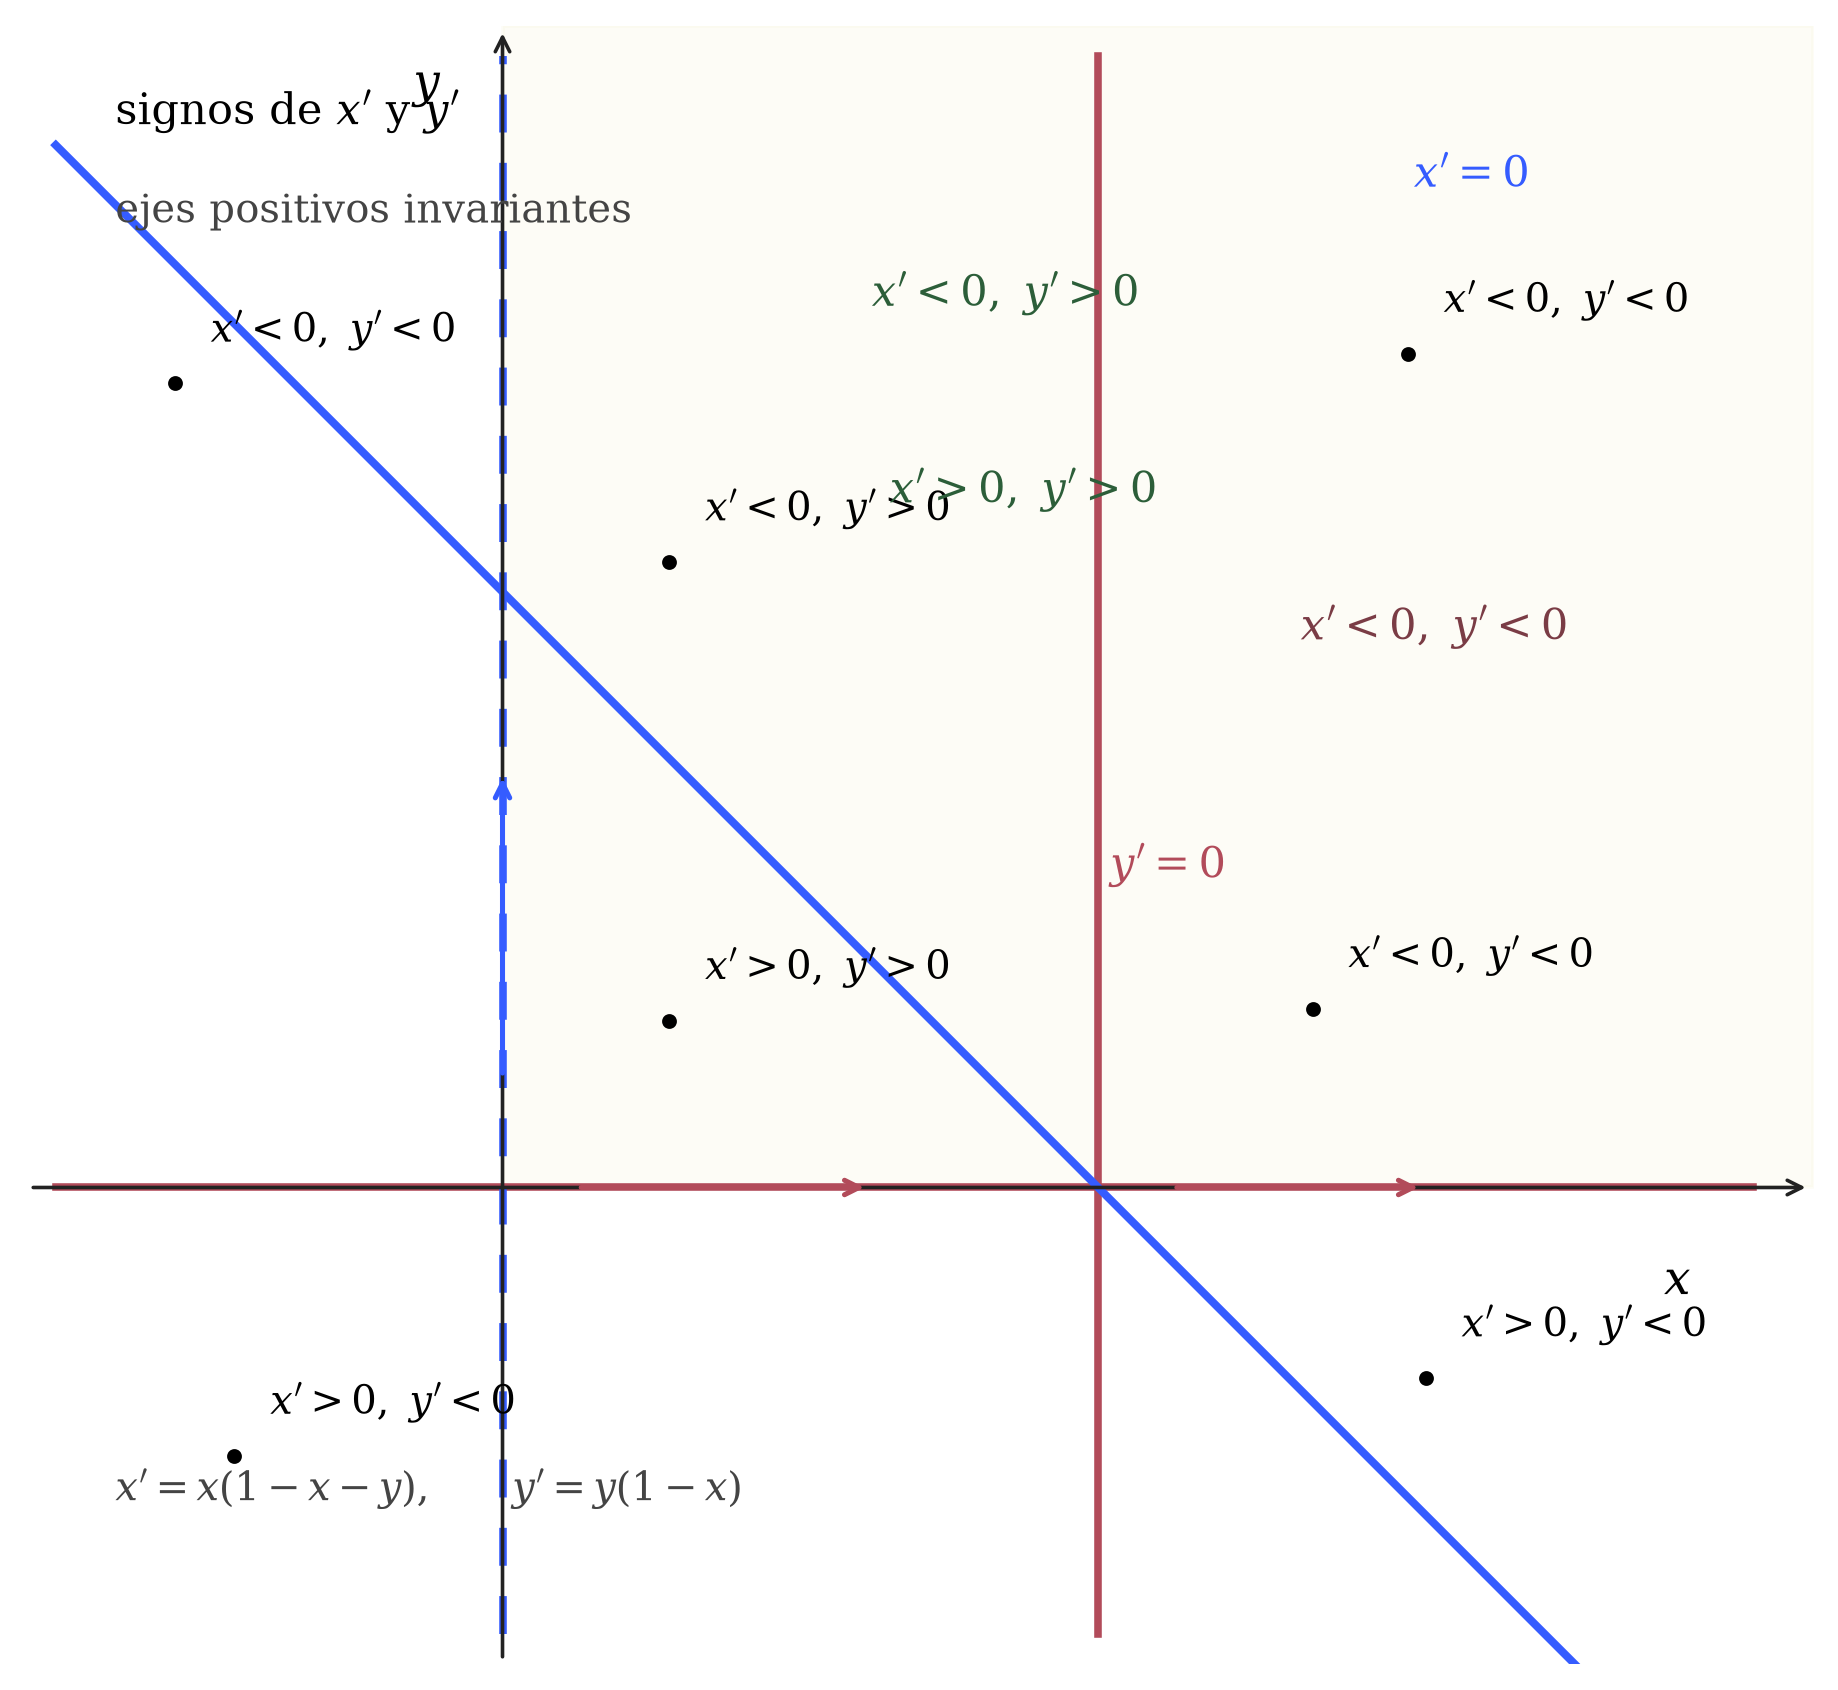
\includegraphics[width=0.92\linewidth]{fig_24_competencia_signos.png}
\end{figure}

% ============================================================
\section{Dinámica de dos poblaciones: modelo depredador-presa}
\label{sec:lotka-volterra}
% ============================================================

Después de estudiar una sola población, pasamos al caso de dos especies
interactuando. El sistema clásico presa--depredador de Lotka--Volterra
\naglecite{§5.1} describe la coevolución de presas $P$ y depredadores $D$
distribuidos uniformemente en un hábitat.

\textbf{Hipótesis del modelo:}
\begin{enumerate}
    \item En ausencia de depredador, la presa crece exponencialmente: $P'=\alpha P$.
    \item En ausencia de presa, el depredador se extingue: $D'=-\gamma D$.
    \item Cuando ambas poblaciones son positivas, los encuentros reducen la presa
          y benefician al depredador en proporción a $PD$.
\end{enumerate}

El sistema resultante es:
\[
\boxed{\frac{dP}{dt}=\alpha P-\beta PD, \qquad \frac{dD}{dt}=-\gamma D+\delta PD,}
\]
con $\alpha,\beta,\gamma,\delta>0$.

\begin{figure}[H]
\centering
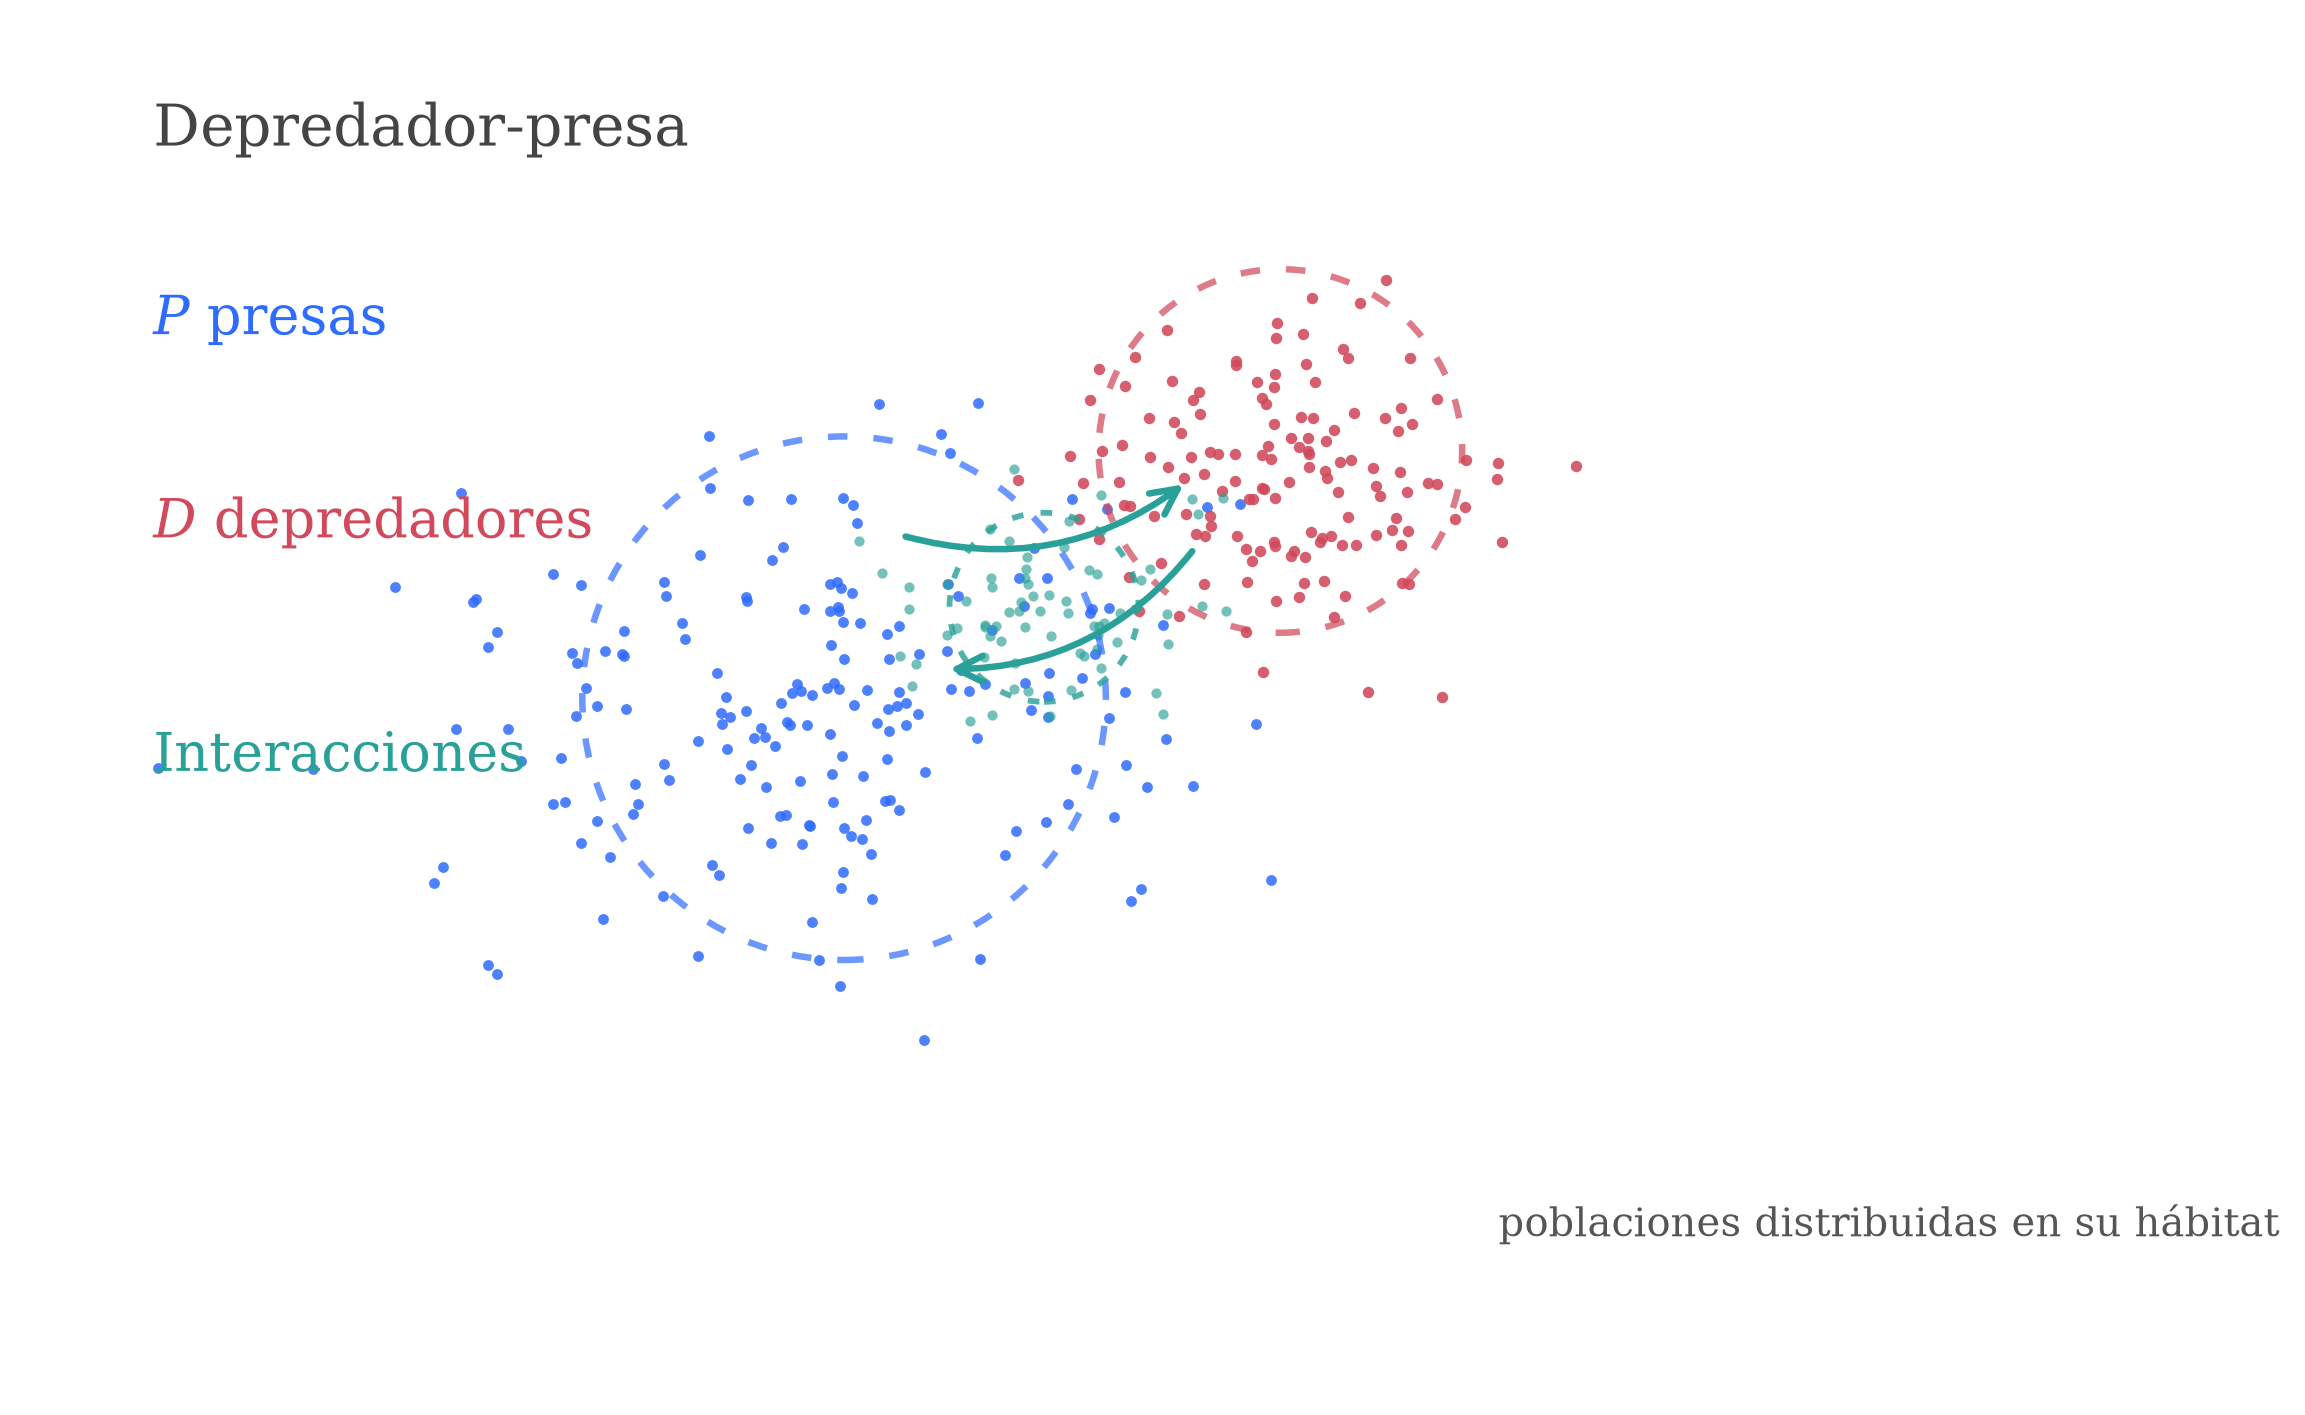
\includegraphics[width=0.92\linewidth]{fig_25_depredador_presa.png}
\caption{Diagrama esquemático del modelo depredador-presa: interacciones entre
las poblaciones $P$ y $D$.}
\end{figure}

\subsection{Adimensionalización del sistema de Lotka--Volterra}

Introduciendo variables características $x_c=\gamma/\delta$, $y_c=\alpha/\beta$,
$t_c=1/\alpha$ (con $P=ux_c$, $D=vy_c$, $t=\tau t_c$) el sistema se reduce a:
\[
\boxed{\frac{du}{d\tau}=u(1-v),\qquad
\frac{dv}{d\tau}=\delta v(u-1),\qquad \delta=\frac{\gamma}{\alpha}.}
\]
El sistema adimensional tiene un solo parámetro $\delta=\gamma/\alpha$ en lugar
de cuatro. Los equilibrios son $(0,0)$ y $(1,1)$.

\subsection{Análisis de isoclinas y signos}

Como los factores $P$ y $D$ aparecen multiplicando en cada ecuación, los ejes
coordenados son invariantes. Las isoclinas nulas del sistema son:
\begin{itemize}
    \item Para $P'$: $P=0$ o $D=\alpha/\beta$ (recta horizontal).
    \item Para $D'$: $D=0$ o $P=\gamma/\delta$ (recta vertical).
\end{itemize}
Estas rectas dividen el primer cuadrante en cuatro regiones. En cada una, el
signo de $P'$ y $D'$ es constante:
\[
0<P<\tfrac{\gamma}{\delta},\;0<D<\tfrac{\alpha}{\beta} \;\Rightarrow\; P'>0,\;D'<0,
\]
\[
0<P<\tfrac{\gamma}{\delta},\;D>\tfrac{\alpha}{\beta} \;\Rightarrow\; P'<0,\;D'<0,
\]
\[
P>\tfrac{\gamma}{\delta},\;0<D<\tfrac{\alpha}{\beta} \;\Rightarrow\; P'>0,\;D'>0,
\]
\[
P>\tfrac{\gamma}{\delta},\;D>\tfrac{\alpha}{\beta} \;\Rightarrow\; P'<0,\;D'>0.
\]

\begin{figure}[H]
\centering
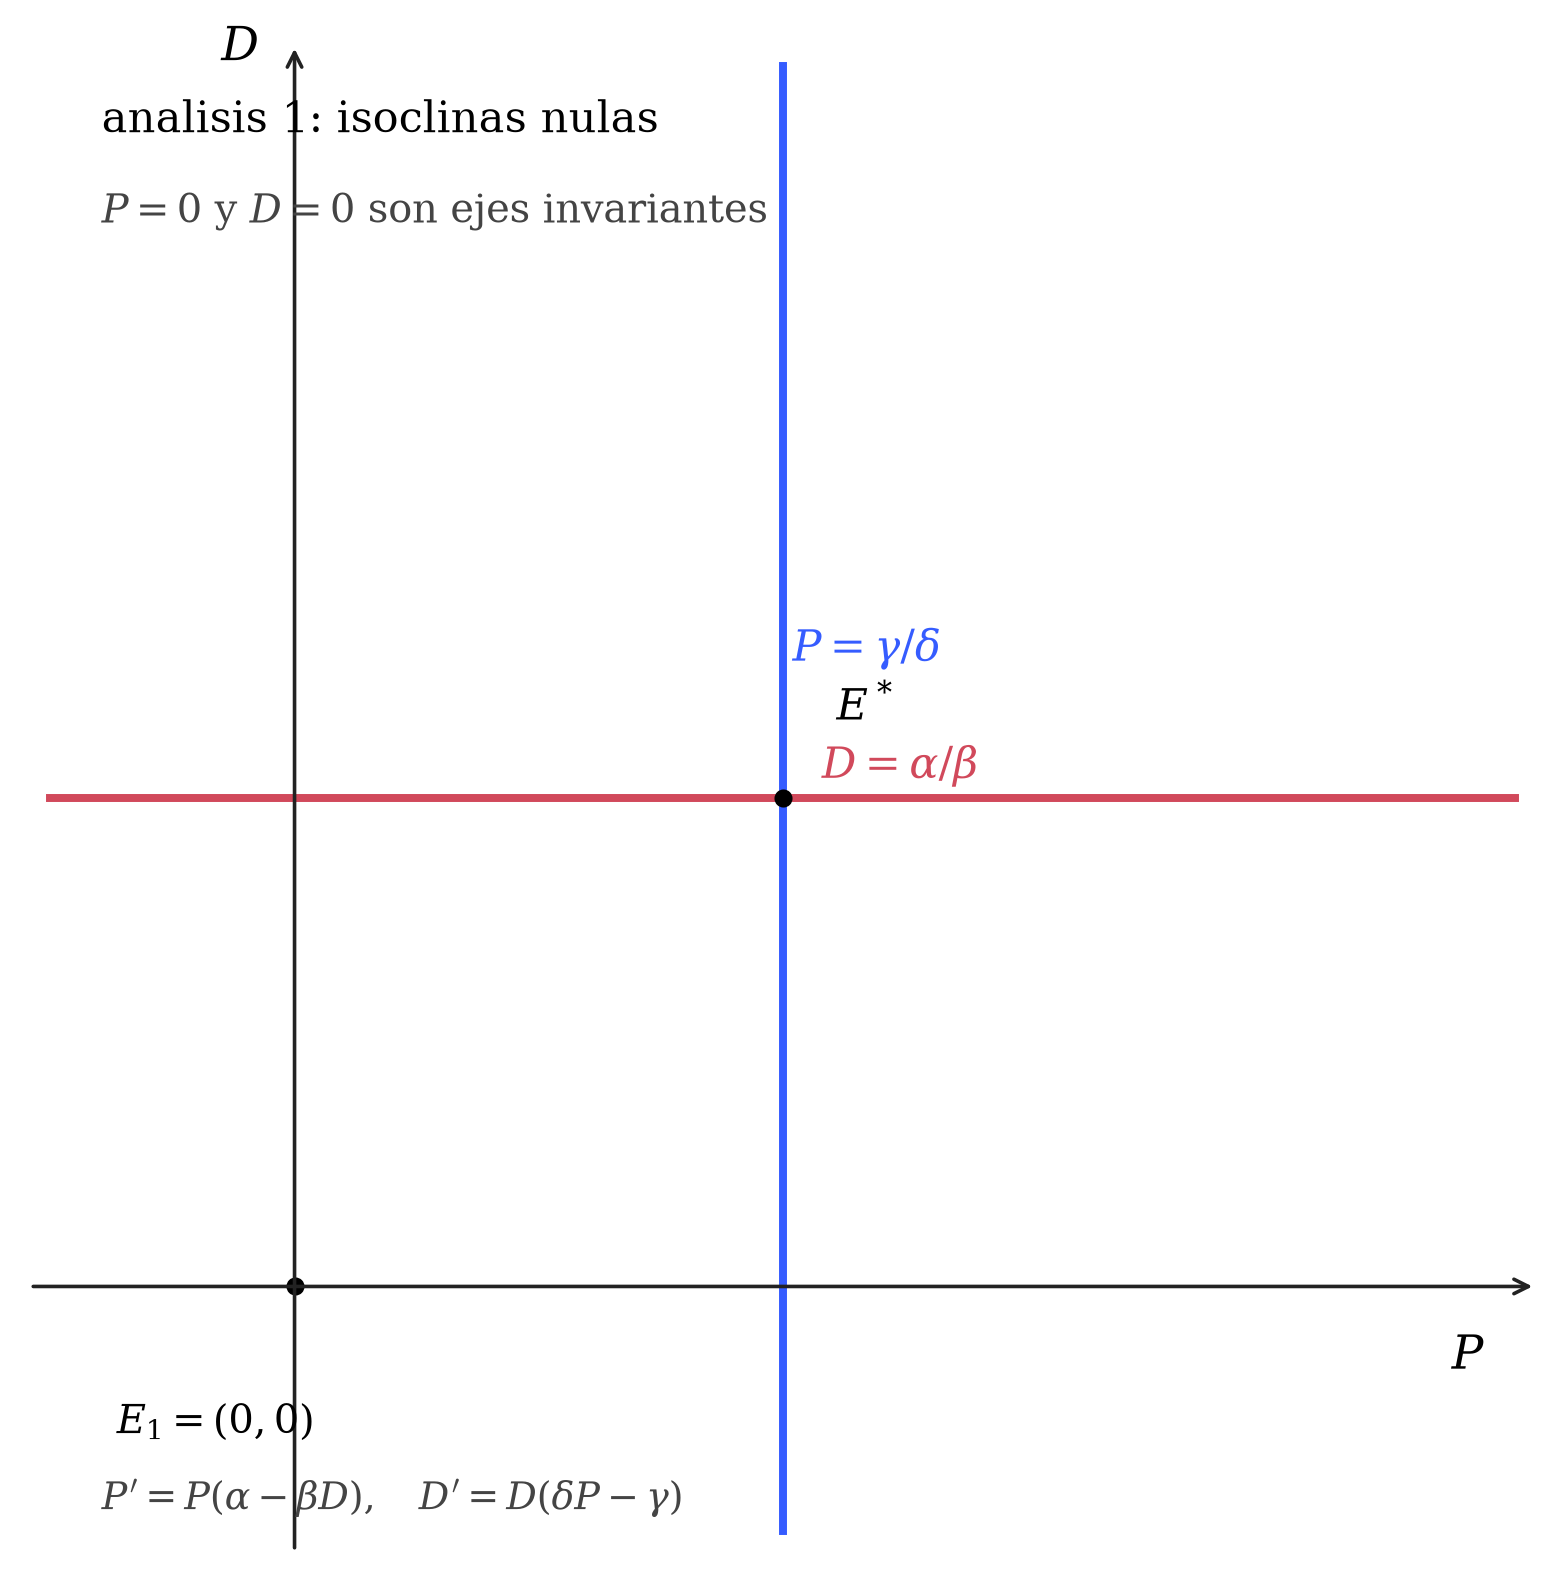
\includegraphics[width=0.92\linewidth]{fig_27_depredador_presa_etapa1.png}
\caption{Primera etapa: ejes invariantes, isoclinas nulas y equilibrios
$E_1=(0,0)$ y $E^*=(\gamma/\delta,\alpha/\beta)$.}
\end{figure}

\begin{figure}[H]
\centering
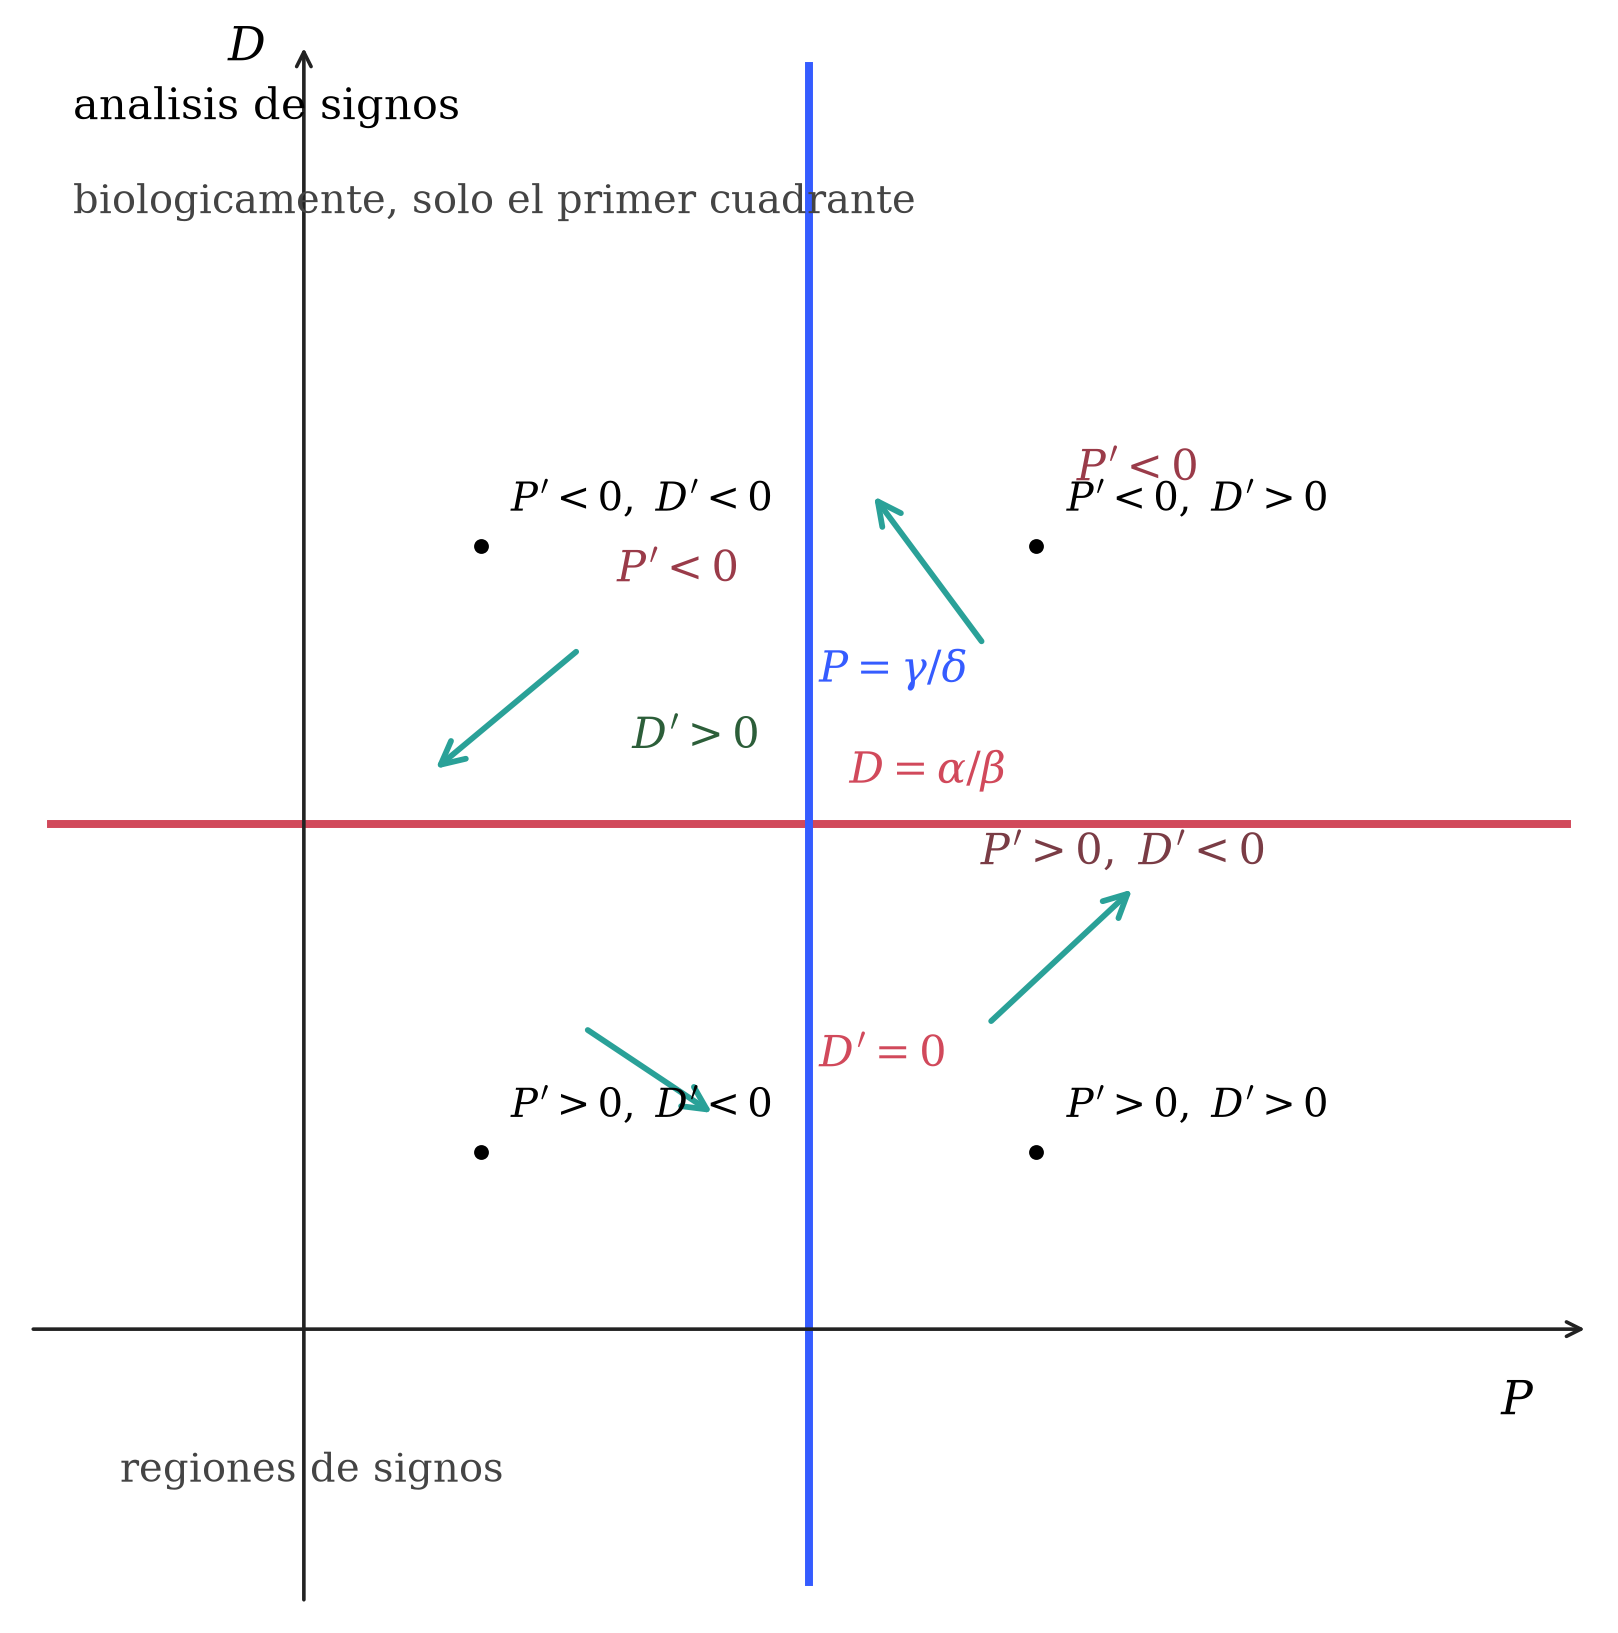
\includegraphics[width=0.92\linewidth]{fig_28_depredador_presa_etapa2.png}
\caption{Segunda etapa: signos de $P'$ y $D'$ en cada región y dirección del flujo.}
\end{figure}

\subsection{Puntos de equilibrio y estabilidad local}

El jacobiano del sistema es
\[
J(P,D)=\begin{pmatrix}\alpha-\beta D & -\beta P \\ \delta D & \delta P-\gamma\end{pmatrix}.
\]

\textbf{Equilibrio de extinción $E_1=(0,0)$:}
\[
J(E_1)=\begin{pmatrix}\alpha & 0 \\ 0 & -\gamma\end{pmatrix}.
\]
Los valores propios son $\lambda_1=\alpha>0$ y $\lambda_2=-\gamma<0$. Por lo tanto,
$E_1$ es hiperbólico y de \textbf{tipo silla}: en ausencia de ambas especies, la
presa crece pero el depredador se extingue, de modo que el origen es un punto de silla.

\textbf{Equilibrio de coexistencia $E^*=\left(\dfrac{\gamma}{\delta},\dfrac{\alpha}{\beta}\right)$:}
\[
J(E^*)=\begin{pmatrix}0 & -\beta\tfrac{\gamma}{\delta} \\ \delta\tfrac{\alpha}{\beta} & 0\end{pmatrix}.
\]
El polinomio característico es
\[
p(\lambda)=\lambda^2+\alpha\gamma=0 \;\Longrightarrow\; \lambda=\pm i\sqrt{\alpha\gamma}.
\]
Los valores propios son puramente imaginarios, así que $E^*$ \textbf{no es hiperbólico}.
El teorema de Hartman-Grobman no es aplicable: la linealización predice un centro,
pero esto no garantiza que el sistema no lineal también lo tenga. Para concluir,
se necesita un argumento diferente: la integral primera.

\begin{figure}[H]
\centering
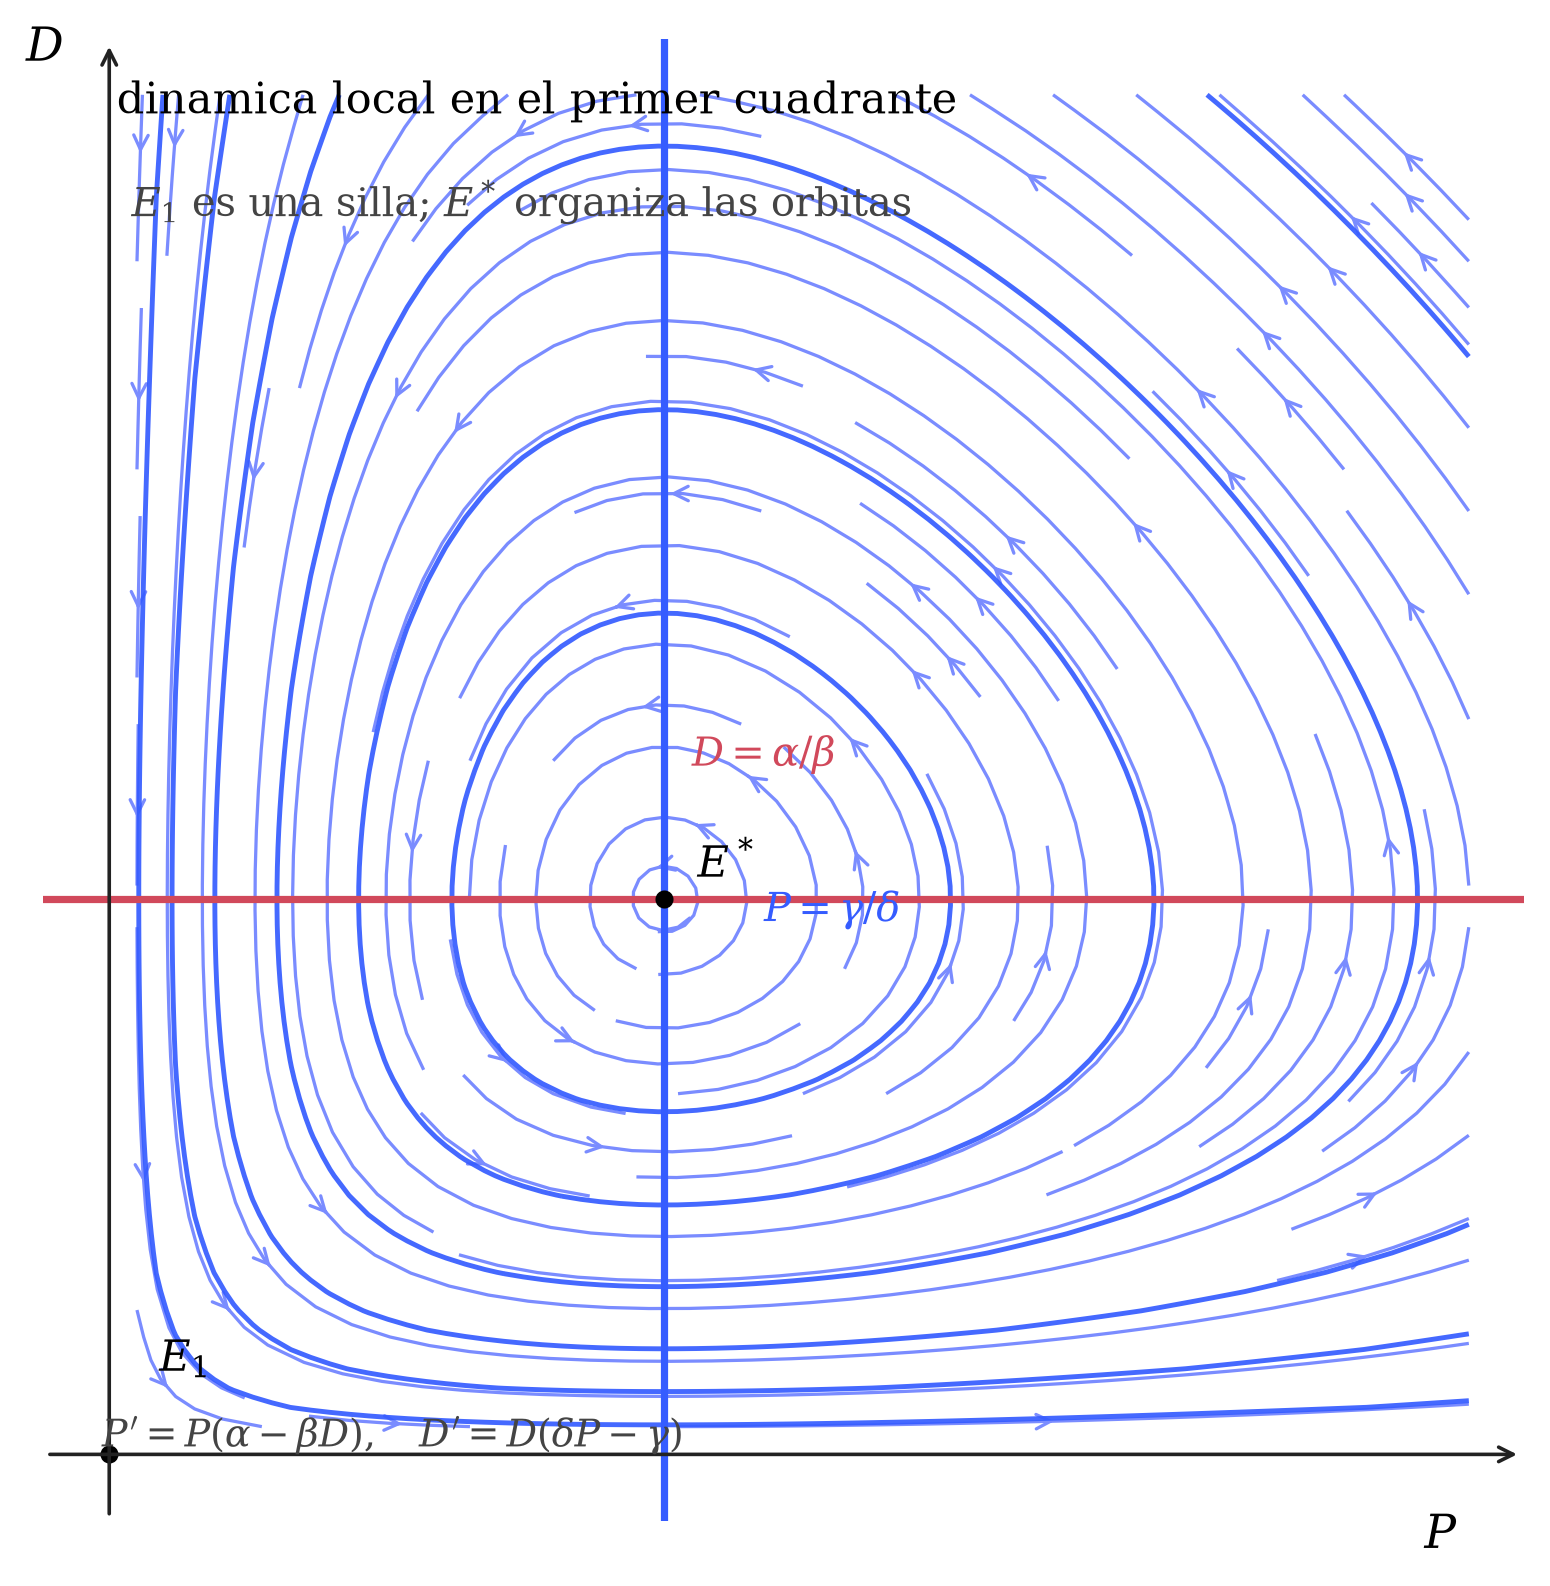
\includegraphics[width=0.92\linewidth]{fig_29_depredador_presa_etapa3.png}
\caption{Tercera etapa: retrato local completo. $E_1$ es una silla; $E^*$ organiza
las órbitas cerradas del modelo clásico.}
\end{figure}

\subsection{Integrales primeras y órbitas cerradas}
\label{sec:integrales-primeras}

Una \textbf{integral primera} es una función conservada a lo largo de las trayectorias,
análoga a la energía en mecánica. Su existencia garantiza que las órbitas son
curvas de nivel de esa función.

\begin{definicion}{Integral primera}{}
Sea $X'=F(X)$ en $\mathbb{R}^n$ con $F$ suficientemente diferenciable.
Una función $H:\mathbb{R}^n\to\mathbb{R}$ es una \textbf{integral primera} del
sistema si $H(X(t))=\text{cte}$ para toda solución $X(t)$, es decir:
\[
\frac{d}{dt}H(X(t)) = \nabla H(X(t))\cdot F(X(t)) = 0.
\]
\end{definicion}

La condición $\nabla H\cdot F=0$ tiene una interpretación geométrica elegante:
el gradiente de $H$, que apunta en la dirección de máximo crecimiento de $H$,
es perpendicular al campo vectorial $F$. Esto equivale a decir que el flujo
es tangente a las curvas de nivel de $H$.

\begin{figure}[H]
\centering
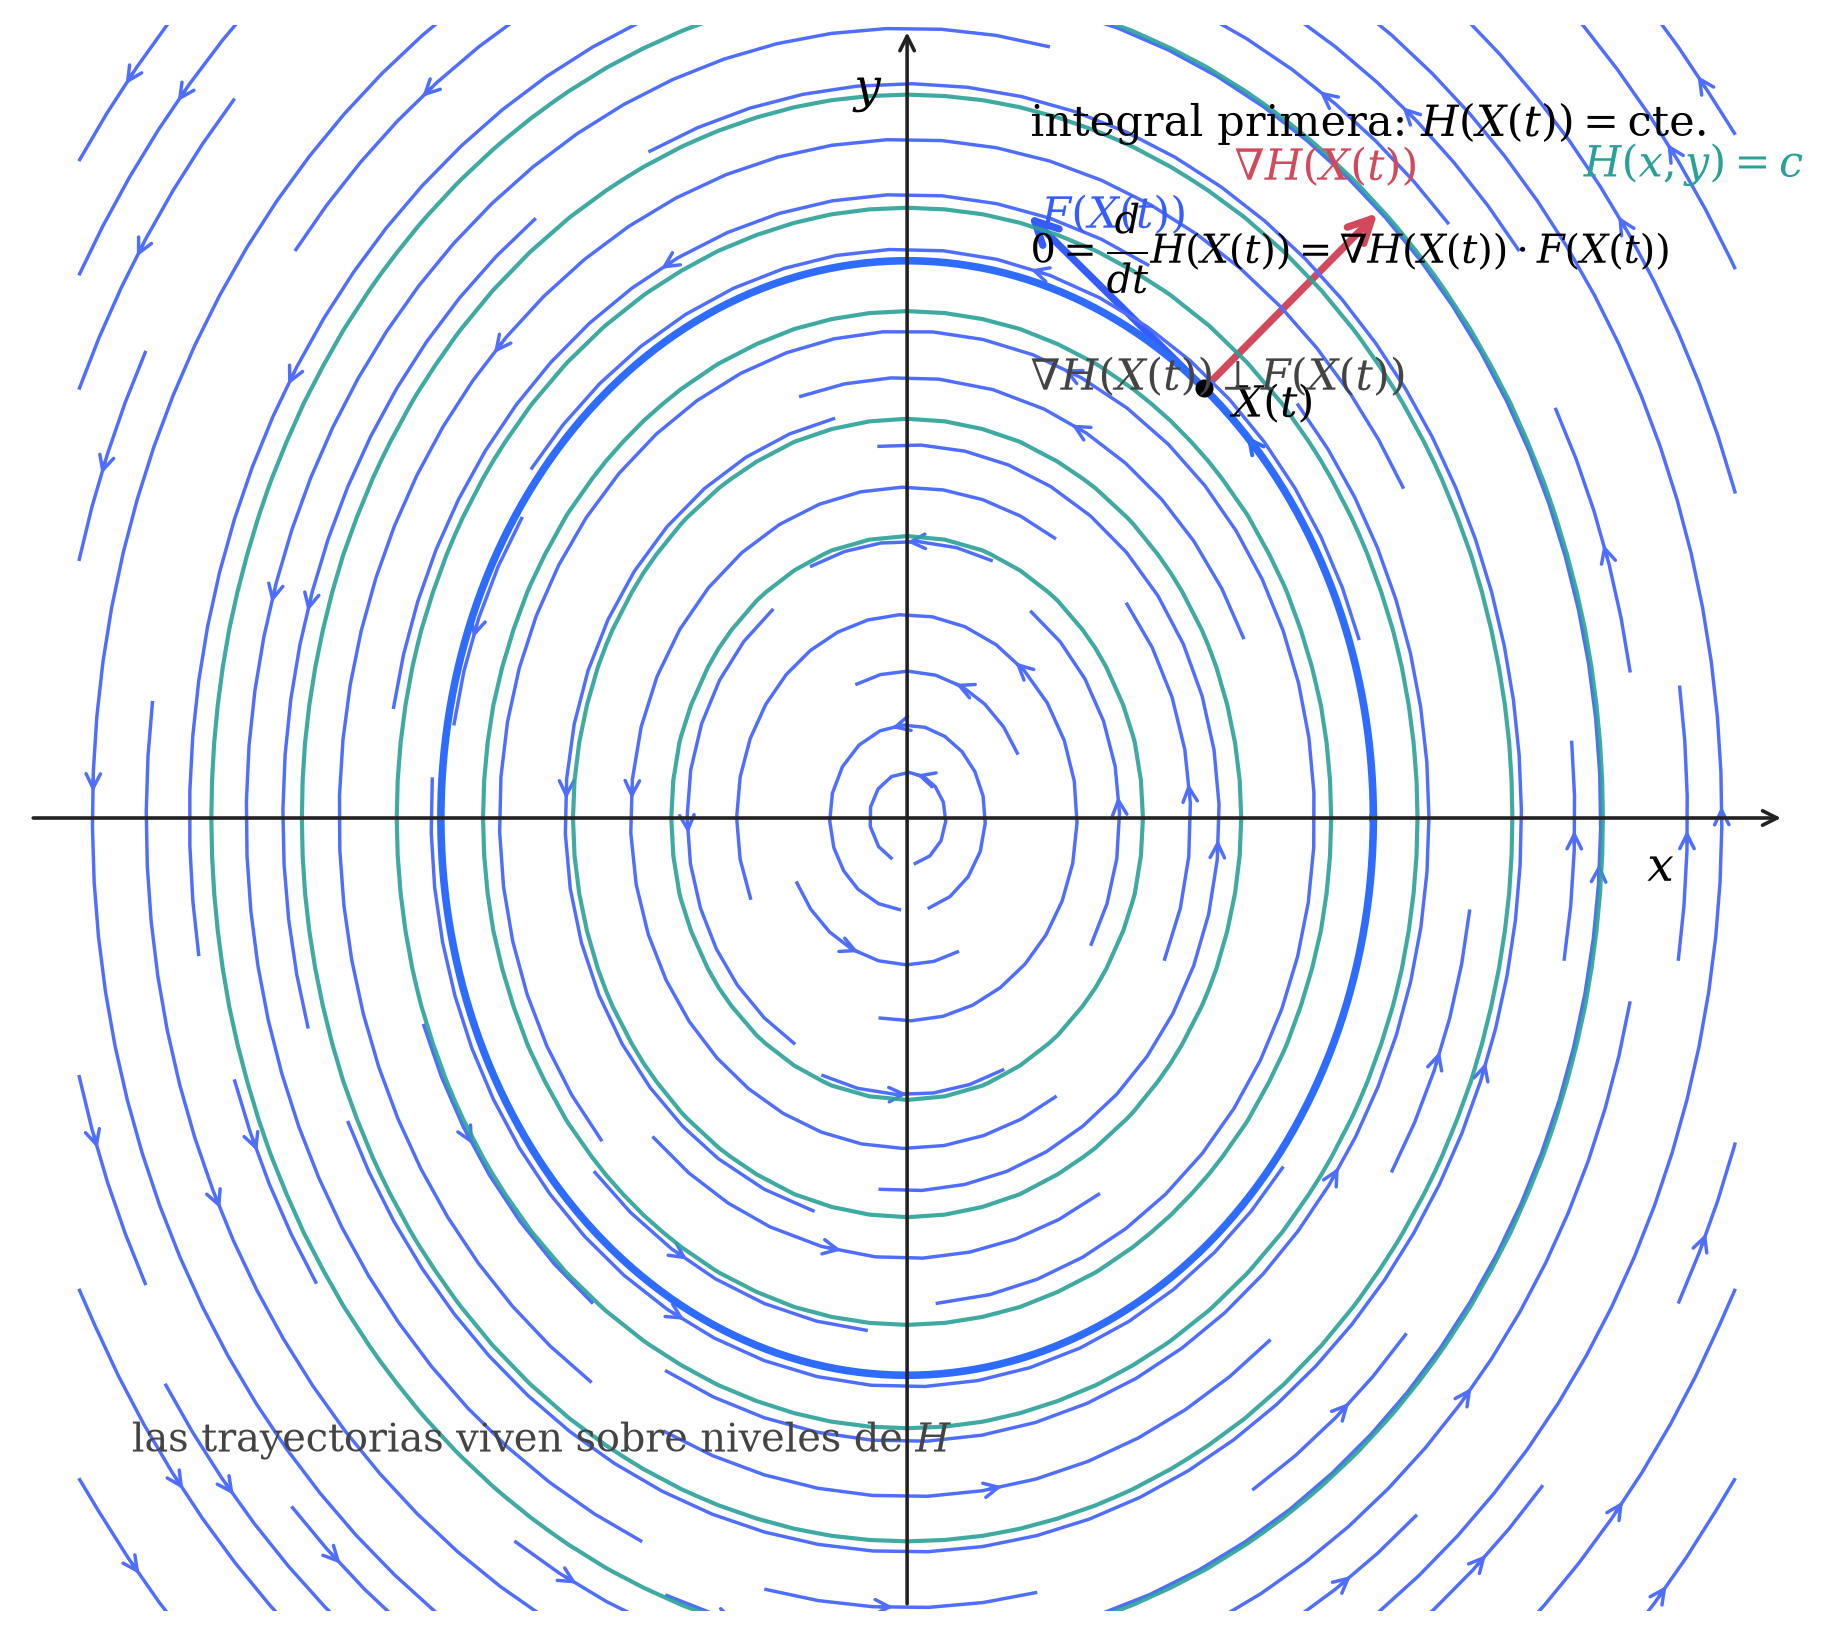
\includegraphics[width=0.92\linewidth]{fig_30_integral_primera_esquema.png}
\caption{Curvas de nivel de $H$ y trayectorias del sistema: $F(X(t))$ es tangente
a las curvas de nivel y $\nabla H(X(t))$ es perpendicular a ellas.}
\end{figure}

\textbf{Derivación de la integral primera de Lotka-Volterra.}
En la región biológicamente relevante $P,D>0$, se puede escribir la relación entre
las componentes eliminando el tiempo:
\[
\frac{dD}{dP}=\frac{D(-\gamma+\delta P)}{P(\alpha-\beta D)}.
\]
Separando variables:
\[
\frac{\alpha-\beta D}{D}\,dD = \frac{-\gamma+\delta P}{P}\,dP.
\]
Integrando ambos lados:
\[
\alpha\ln D - \beta D = -\gamma\ln P + \delta P + C.
\]
Reorganizando, se obtiene la integral primera:
\[
\boxed{H(P,D)=-\gamma\ln P+\delta P+\beta D-\alpha\ln D = \text{cte}.}
\]
Sus curvas de nivel son exactamente las órbitas del sistema. Como $H$ es una función
estrictamente convexa con mínimo en $E^*$, las curvas de nivel son cerradas alrededor
de $E^*$: las soluciones son periódicas para cualquier condición inicial positiva.

\begin{figure}[H]
\centering

\includegraphics[width=0.92\linewidth]{fig_32_depredador_presa_integral_derivacion.png}
\caption{Derivación algebraica de la integral primera: de la ecuación $dD/dP$
a la expresión final de $H(P,D)$.}
\end{figure}

\subsection{Verificación: $H$ es integral primera}

Tomemos
\[
H(P,D)=\alpha \ln D-\beta D-\delta P+\gamma \ln P
\]
y el sistema
\[
(*)\begin{cases}
\dfrac{dP}{dt}=\alpha P-\beta PD\\[4pt]
\dfrac{dD}{dt}=-\gamma D+\delta PD.
\end{cases}
\]

\textbf{Afirmación:} $H(P,D)$ es una integral primera de $(*)$, es decir, $H$ es
constante a lo largo de cualquier solución de $(*)$.

\textbf{Demostración.} Sea $X(t)=(P(t),D(t))$ una solución de $(*)$. Calculamos
la derivada de Lie de $H$ a lo largo de $X(t)$:
\[
\dot{H}(t)
\stackrel{\mathrm{def}}{=}\frac{d}{dt}H(X(t))
=\nabla H(X(t))\cdot X'(t)
=\left(\frac{\partial H}{\partial P},\frac{\partial H}{\partial D}\right)\cdot\bigl(P'(t),D'(t)\bigr).
\]
Calculando las derivadas parciales de $H$:
\[
\frac{\partial H}{\partial P}=-\delta+\frac{\gamma}{P},\qquad
\frac{\partial H}{\partial D}=\frac{\alpha}{D}-\beta.
\]
Sustituyendo el sistema $(*)$:
\[
\dot{H}
=\left(-\delta+\frac{\gamma}{P}\right)(\alpha P-\beta PD)+
\left(\frac{\alpha}{D}-\beta\right)(-\gamma D+\delta PD).
\]
Expandiendo término a término:
\[
\dot{H}
=-\delta\alpha P+\delta\beta PD+\gamma\alpha-\gamma\beta D
-\alpha\gamma+\alpha\delta P+\beta\gamma D-\beta\delta PD.
\]
Todos los términos se cancelan:
\[
\dot{H}=(-\delta\alpha P+\alpha\delta P)+(\delta\beta PD-\beta\delta PD)
+(\gamma\alpha-\alpha\gamma)+(-\gamma\beta D+\beta\gamma D)=0.
\]
Por lo tanto $H(X(t))=\text{cte}$ para toda solución positiva. $\square$

\textbf{Interpretación geométrica.} La condición $\dot{H}=0$ equivale a
$\nabla H(X)\cdot F(X)=0$: el gradiente de $H$, que apunta en la dirección de
máximo crecimiento de $H$, es perpendicular al campo vectorial $F$. Esto
significa que el flujo es tangente a las curvas de nivel de $H$, y la trayectoria
$X(t)$ se mueve sobre una de esas curvas sin abandonarla jamás.

Como $H$ es estrictamente convexa con mínimo en $E^*=(\gamma/\delta,\alpha/\beta)$,
sus curvas de nivel son cerradas alrededor de $E^*$: todas las soluciones con
condición inicial positiva son periódicas y orbitan alrededor del equilibrio de
coexistencia.

\begin{figure}[H]
\centering
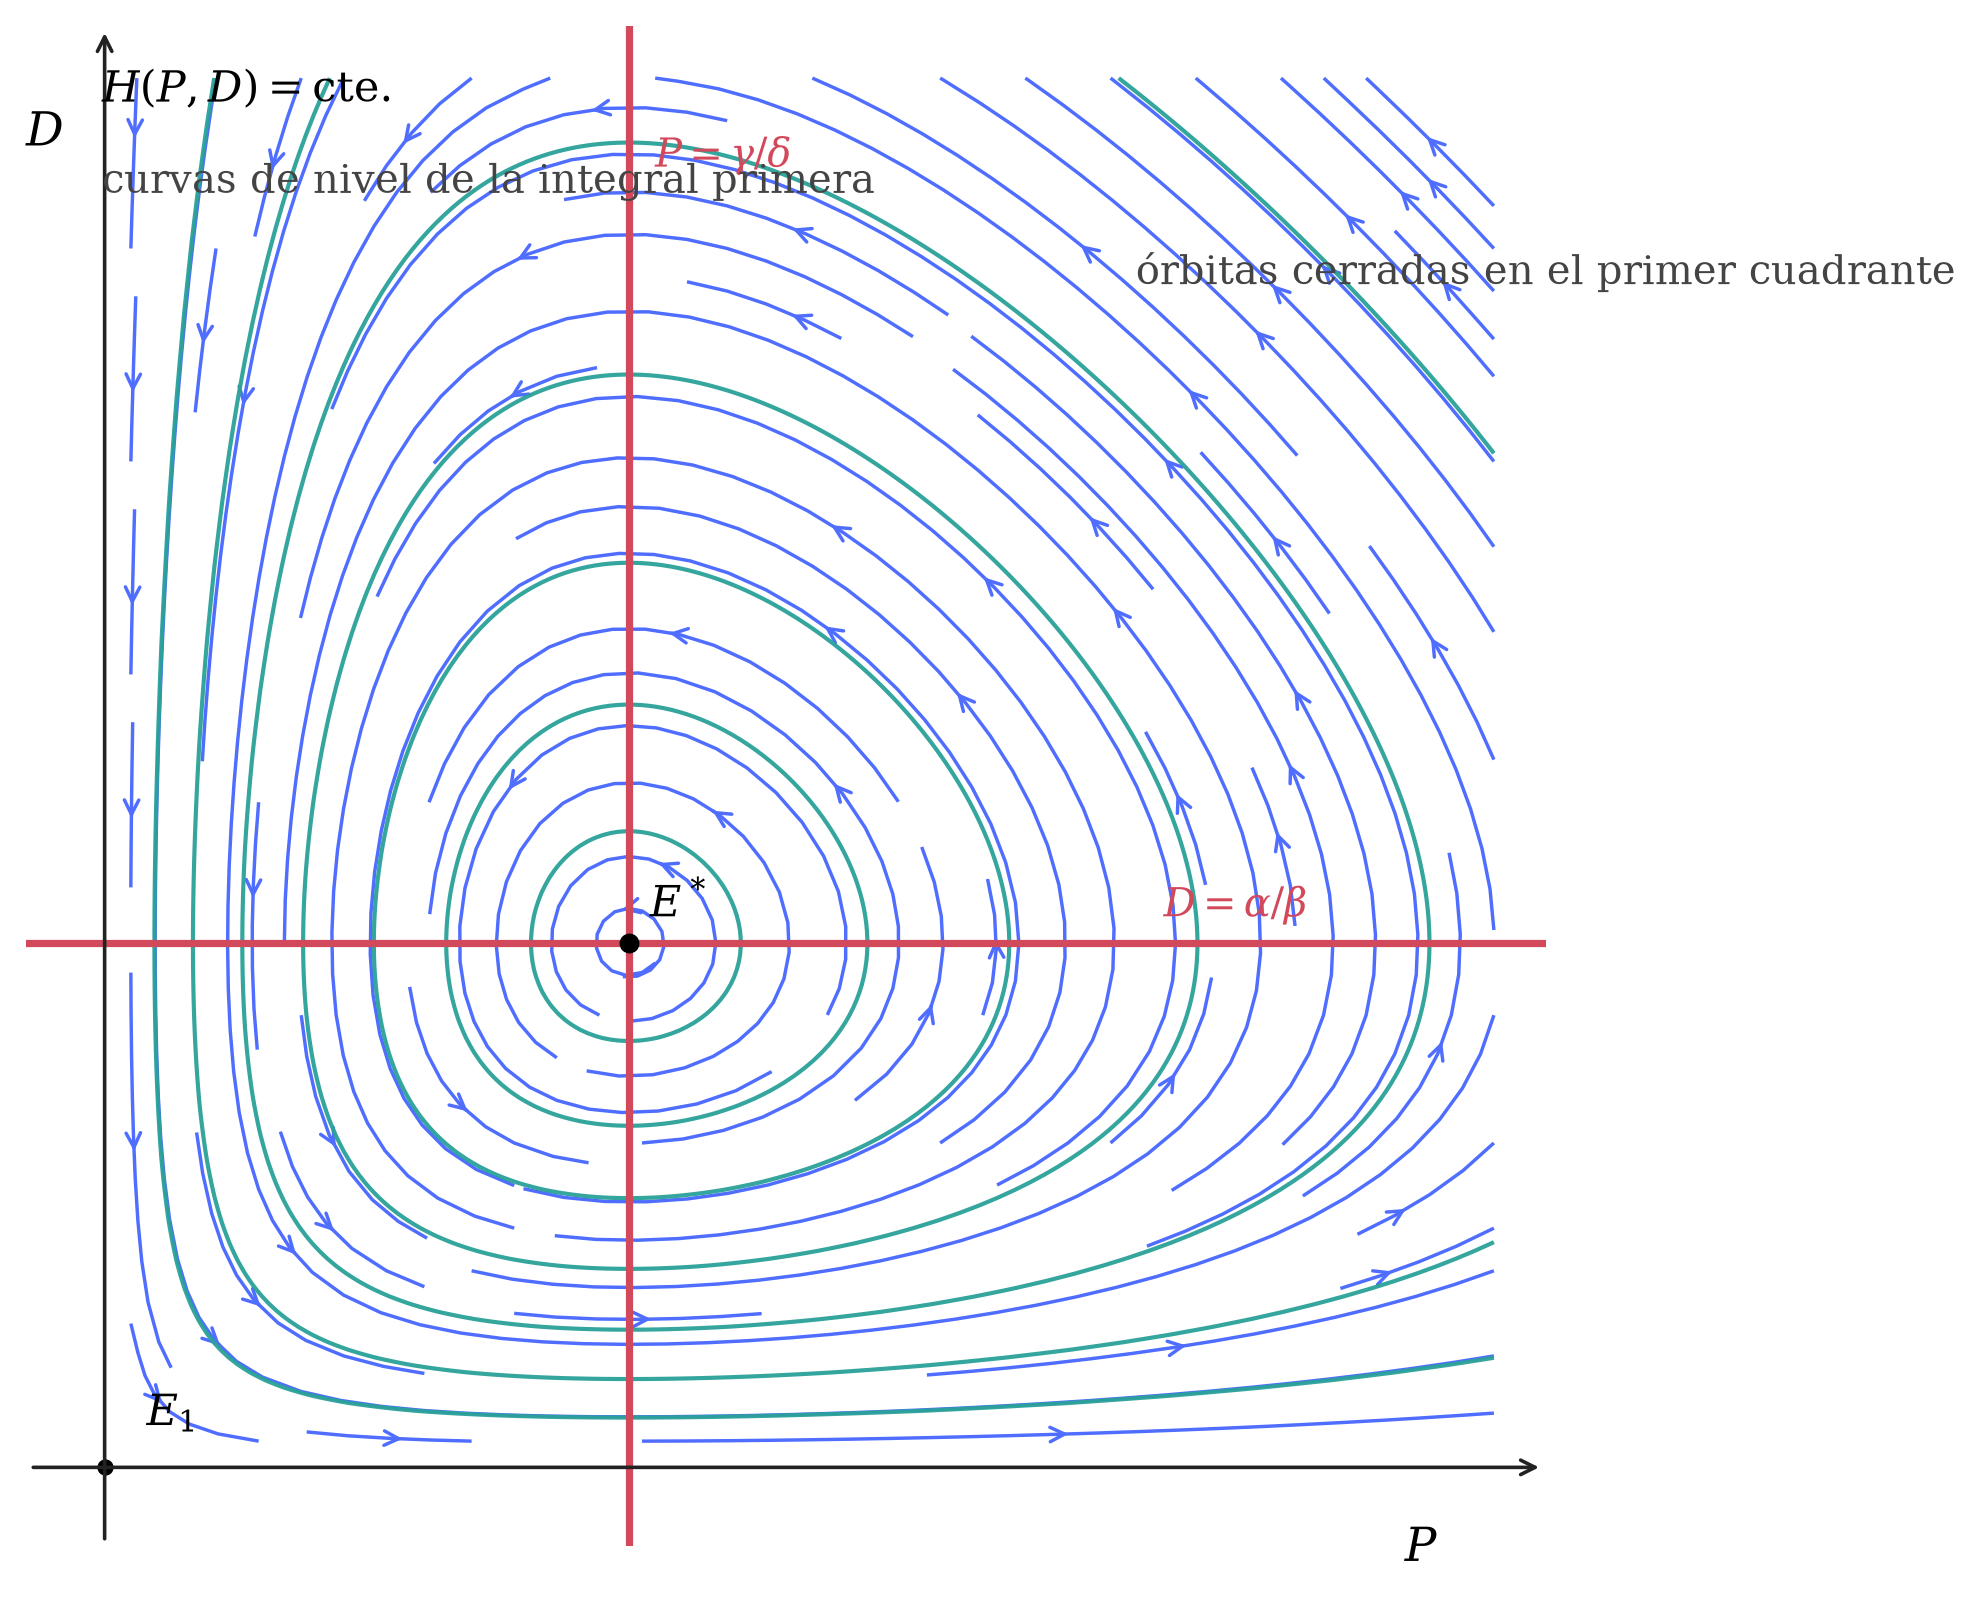
\includegraphics[width=0.92\linewidth]{fig_33_depredador_presa_integral_orbitas.png}
\caption{Campo vectorial con curvas de nivel de $H(P,D)$: $E_1=(0,0)$ es silla,
$E^*=(\gamma/\delta,\alpha/\beta)$ es el mínimo de $H$ y las órbitas son cerradas.}
\end{figure}

\textbf{Interpretación temporal.} Visto en el tiempo, el movimiento sobre las
curvas de nivel de $H$ se traduce en oscilaciones desfasadas: primero crece la
presa, esto permite que el depredador aumente, la abundancia del depredador reduce
la presa, y la escasez de presa hace disminuir al depredador, reiniciando el ciclo.

\begin{figure}[H]
\centering
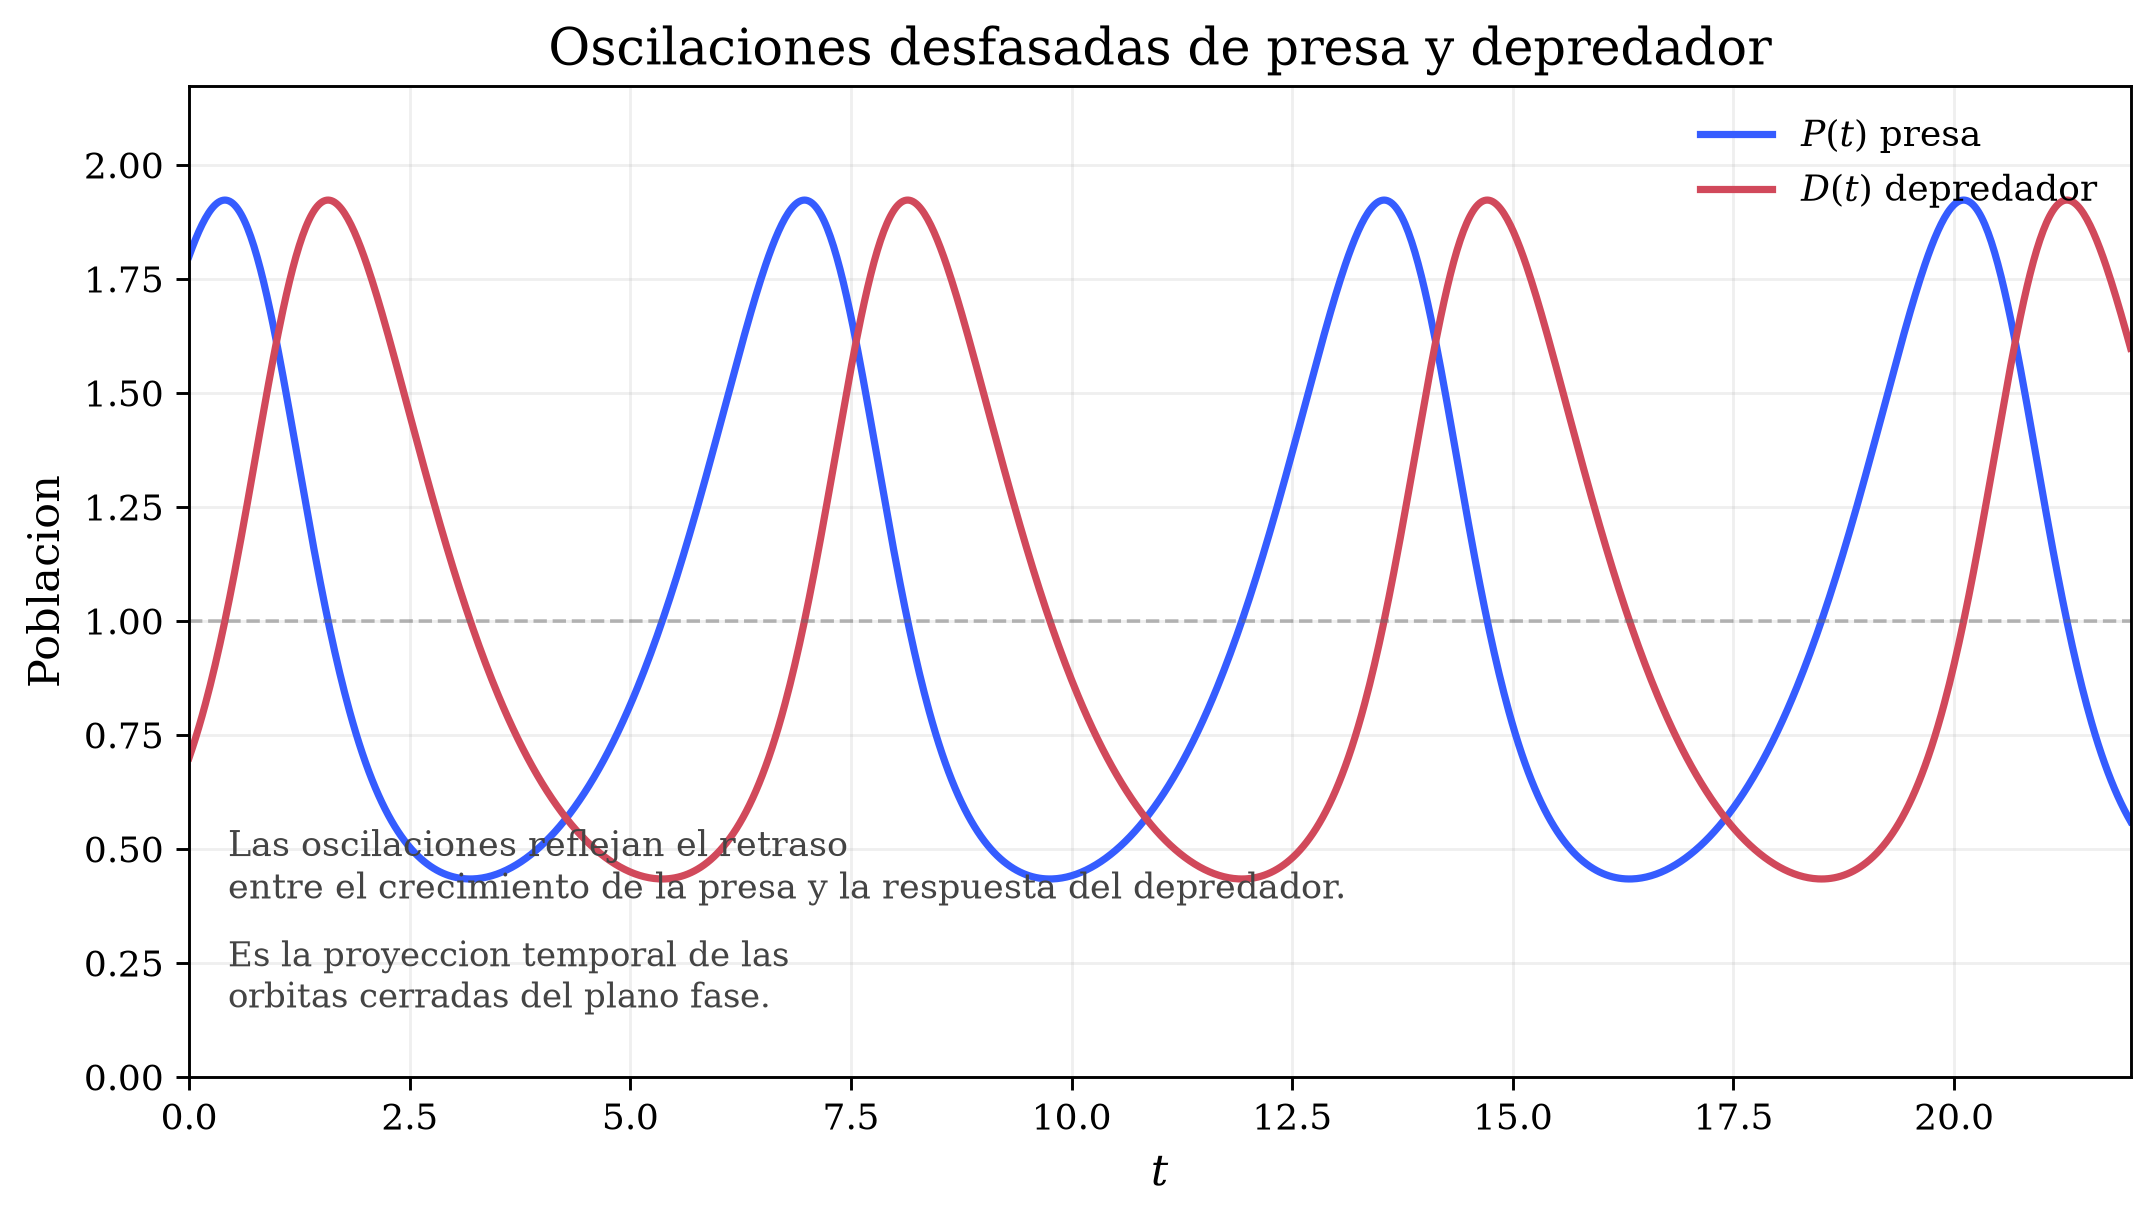
\includegraphics[width=0.92\linewidth]{fig_34_depredador_presa_series_tiempo.png}
\caption{Evolución temporal de $P(t)$ y $D(t)$: las dos poblaciones oscilan con
desfase, en coherencia con el retrato de fases.}
\end{figure}

\begin{figure}[H]
\centering
\begin{minipage}[t]{0.56\textwidth}
\centering
\begin{tikzpicture}[scale=0.95]
\draw[->] (0,0) -- (7,0) node[right] {$P$};
\draw[->] (0,0) -- (0,5.5) node[above] {$D$};
\draw[thick,blue!70!black] (0,4.6) -- (4.6,0)
    node[pos=0.85,above] {$D=\frac{r}{\beta}\!\left(1-\frac{P}{K}\right)$};
\draw[thick,red!70!black,dashed] (3.0,0) -- (3.0,5.2) node[above] {$P=\frac{\gamma}{\delta}$};
\fill (3.0,1.55) circle (2pt) node[above right] {$E^*$};
\foreach \x/\y in {0.8/0.8,1.5/1.2,2.0/2.7,3.8/1.0,4.8/2.8,2.0/4.0,4.8/4.2}{
  \pgfmathsetmacro{\u}{(\x*(1-\x/4)-0.45*\x*\y)}
  \pgfmathsetmacro{\v}{(-\y+0.35*\x*\y)}
  \pgfmathsetmacro{\len}{sqrt(\u*\u+\v*\v)}
  \draw[-{Latex[length=2mm]},gray!70] (\x,\y)--++({0.48*\u/\len},{0.48*\v/\len});
}
\end{tikzpicture}
\end{minipage}
\hfill
\begin{minipage}[t]{0.40\textwidth}
\centering
\begin{tikzpicture}
\begin{axis}[
    width=\linewidth, height=4.8cm,
    xmin=0,xmax=5,ymin=0,ymax=5,
    axis lines=middle,
    xlabel={$P$},ylabel={$f(P)$},
    tick style={draw=none},xtick=\empty,ytick=\empty,
    legend style={draw=none,at={(0.02,0.98)},anchor=north west,font=\small}
]
\addplot[thick,red!70!black,domain=0:5,samples=200]{x};
\addlegendentry{$f=P$}
\addplot[thick,blue!70!black,domain=0:5,samples=200]{x/(1+x)};
\addlegendentry{$f=\frac{P}{1+P}$}
\end{axis}
\end{tikzpicture}
\end{minipage}
\caption{Plano de fases presa-depredador (versión generalizada con capacidad de
carga) y respuestas funcionales típicas: lineal $f=P$ (Lotka-Volterra clásico)
y saturada $f=P/(1+P)$ (Holling tipo II).}
\end{figure}

\subsection{Cosecha en el modelo logístico: perspectiva de integrales}

Consideremos el modelo logístico con cosecha constante:
\[
p'=\alpha p\!\left(1-\frac{p}{k}\right)-H.
\]
Definiendo $f(p)=\alpha p(1-p/k)$, la dinámica se determina comparando la
curva de crecimiento $f(p)$ con el nivel de cosecha $H$.

\begin{figure}[H]
\centering
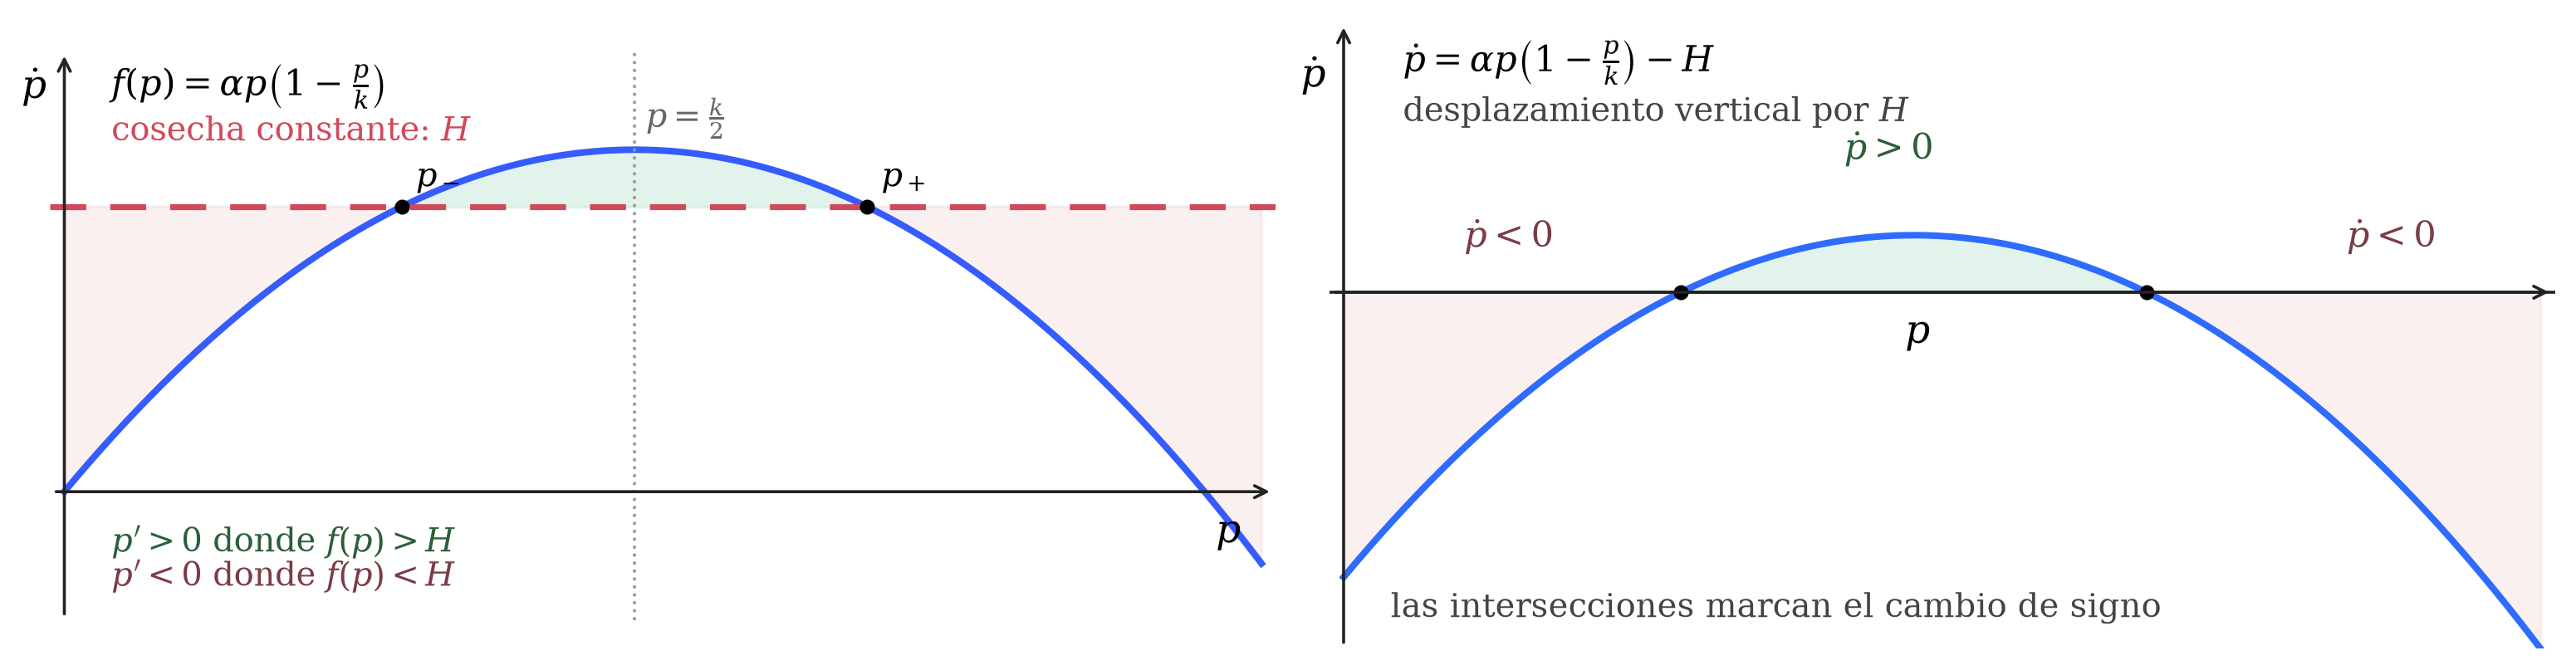
\includegraphics[width=0.92\linewidth]{fig_31_cosecha_logistica.png}
\caption{Izquierda: curva de crecimiento logístico $f(p)$ y recta de cosecha $H$.
Derecha: función neta $p'=f(p)-H$ con sus ceros y signos. Los ceros son los
equilibrios y su estabilidad se lee del signo de la derivada.}
\end{figure}

% ============================================================
\section{Sistemas de tres variables y planos invariantes}
\label{sec:tres-variables}
% ============================================================

Muchos sistemas ecológicos involucran tres especies o tres variables de estado.
Un sistema de la forma
\begin{align*}
x_1' &= x_1 f_1(x_1,x_2,x_3),\\
x_2' &= x_2 f_2(x_1,x_2,x_3),\\
x_3' &= x_3 f_3(x_1,x_2,x_3),
\end{align*}
tiene una propiedad fundamental de invarianza: si alguna variable se anula,
su derivada también se anula, por lo que no puede cambiar de signo.

En particular:
\begin{itemize}
    \item $x_1=0 \Rightarrow x_1'=0$: el plano $x_2 x_3$ es invariante.
    \item $x_2=0 \Rightarrow x_2'=0$: el plano $x_1 x_3$ es invariante.
    \item $x_3=0 \Rightarrow x_3'=0$: el plano $x_1 x_2$ es invariante.
\end{itemize}
\textbf{Por consiguiente, el primer octante} $\{x_1,x_2,x_3\geq 0\}$
\textbf{es invariante}: si el sistema empieza con variables no negativas
(poblaciones, concentraciones), permanece en esa región para todo tiempo.
Esta propiedad simplifica enormemente el análisis y garantiza la relevancia
biológica de las soluciones.

\begin{figure}[H]
\centering
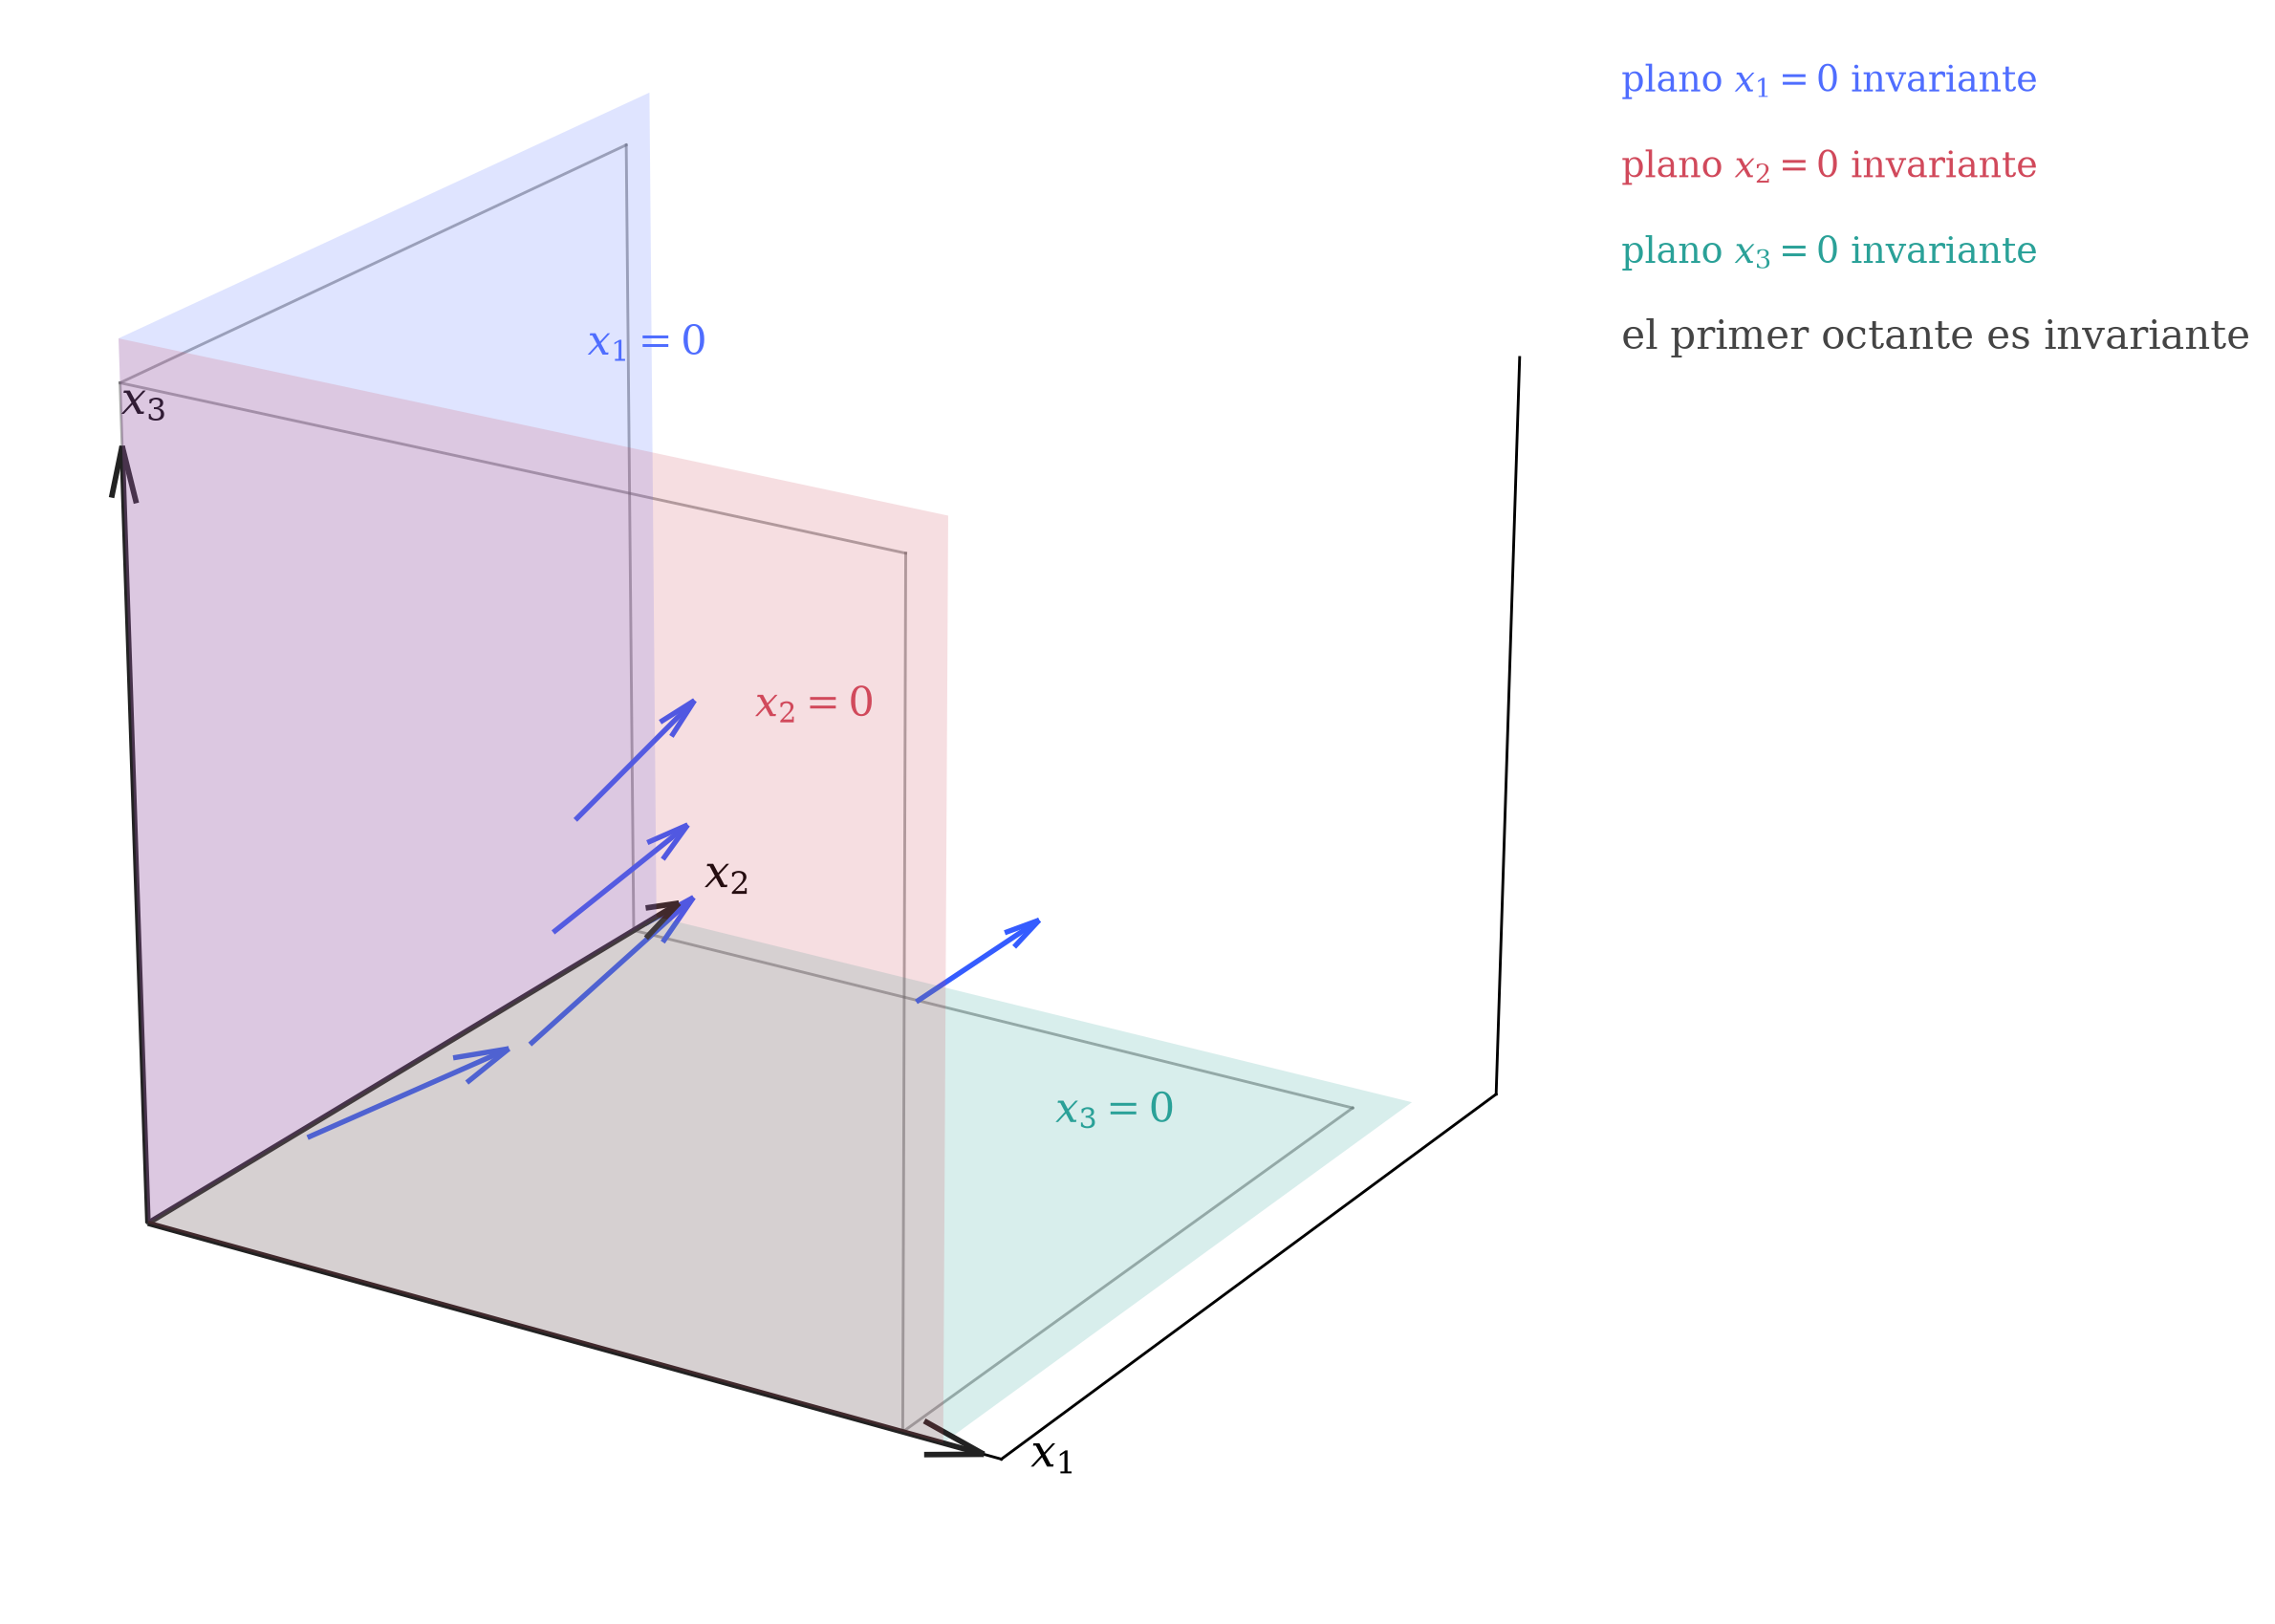
\includegraphics[width=0.92\linewidth]{fig_26_octante_invariante.png}
\caption{El primer octante es invariante: las caras del octante son planos
invariantes y las trayectorias que comienzan en el interior permanecen en él.}
\end{figure}

\naglecite{cap.~12: en sistemas de mayor dimensión, los subespacios invariantes
simplifican el análisis global.}

% ============================================================
\section{Modelos de dos especies en competencia}
\label{sec:competencia}
% ============================================================

Cuando dos especies compiten por los mismos recursos, las interacciones
son recíprocamente perjudiciales. El primer modelo captura esto con términos
multiplicativos, mientras que el segundo incorpora la saturación logística.

\textbf{Modelo 1: crecimiento multiplicativo.}
\[
\begin{cases}
\dfrac{dN_1}{dt}=r_1 N_1 - \beta N_1 N_2,\\[4pt]
\dfrac{dN_2}{dt}=r_2 N_2 - \delta N_1 N_2.
\end{cases}
\]
Este modelo es análogo al de Lotka-Volterra pero con interacciones simétricamente
negativas para ambas especies.

\textbf{Modelo 2: crecimiento logístico con competencia.}
\[
\begin{cases}
\dfrac{dN_1}{dt}=r_1 N_1\!\left(1-\dfrac{N_1}{K_1}\right)-\beta N_1 N_2,\\[4pt]
\dfrac{dN_2}{dt}=r_2 N_2\!\left(1-\dfrac{N_2}{K_2}\right)+\delta N_1 N_2.
\end{cases}
\]
Aquí cada especie tiene capacidad de carga propia $K_1$, $K_2$ y la interacción
modifica el crecimiento de forma asimétrica según los signos de $\beta$ y $\delta$.
El resultado biológico depende de si los coeficientes de competencia permiten
la coexistencia o si una especie desplaza a la otra.

\subsection{Sistema adimensionalizado y significado biológico}

Normalizando cada población por su propia capacidad de carga ($u=N_1/K_1$,
$v=N_2/K_2$) y el tiempo por la tasa de crecimiento de la primera especie
($\tau=r_1 t$), el Modelo~2 se reduce a la forma estándar:
\[
\boxed{u' = u(1-u-Av),\qquad v' = \rho\, v(1-v-Bu).}
\]

\textbf{Significado de los parámetros:}
\begin{itemize}
    \item $u$, $v$: densidades poblacionales adimensionales (normalizadas por la
          capacidad de carga de cada especie; $u=1$ significa que la especie 1
          está en su capacidad de carga).
    \item $A$: coeficiente de competencia interespecífica de $v$ sobre $u$; mide
          cuánto inhibe la presencia de la especie 2 el crecimiento de la especie 1.
          Si $A>1$, la especie 2 es un competidor más dañino para la especie 1 que
          los propios individuos de la especie 1.
    \item $B$: coeficiente de competencia interespecífica de $u$ sobre $v$; papel
          simétrico al de $A$.
    \item $\rho=r_2/r_1$: razón de tasas de crecimiento intrínsecas; si $\rho>1$
          la especie 2 crece más rápido en ausencia de competencia.
\end{itemize}

\subsection{Isoclinas nulas y puntos de equilibrio}

\textbf{Isoclinas nulas:}
\begin{itemize}
    \item Para $u'=0$: \quad $u=0$ \quad o \quad $v=\dfrac{1-u}{A}$
          (recta con interceptos $(1,0)$ y $(0,1/A)$).
    \item Para $v'=0$: \quad $v=0$ \quad o \quad $v=1-Bu$
          (recta con interceptos $(1/B,0)$ y $(0,1)$).
\end{itemize}

\textbf{Puntos de equilibrio.} Combinando las condiciones $u'=0$ y $v'=0$:

\begin{itemize}
    \item $E_1=(0,0)$: extinción de ambas especies.
    \item $E_2=(0,1)$: extinción de la especie 1, especie 2 en su capacidad de carga.
    \item $E_3=(1,0)$: extinción de la especie 2, especie 1 en su capacidad de carga.
    \item $E^*$: coexistencia interior, solución del sistema lineal
\[
u + Av = 1,\qquad Bu + v = 1,
\]
que en forma matricial es
\[
\underbrace{\begin{pmatrix}1 & A\\ B & 1\end{pmatrix}}_{\Delta}
\begin{pmatrix}u\\v\end{pmatrix}
=\begin{pmatrix}1\\1\end{pmatrix}.
\]
El determinante es $\det\Delta=1-AB$. Si $AB\neq 1$, existe una única solución:
\[
\begin{pmatrix}u\\v\end{pmatrix}
=\frac{1}{1-AB}
\begin{pmatrix}1 & -A\\-B & 1\end{pmatrix}
\begin{pmatrix}1\\1\end{pmatrix}
=\frac{1}{1-AB}\begin{pmatrix}1-A\\1-B\end{pmatrix}.
\]
Por lo tanto:
\[
\boxed{E^*=\left(\frac{1-A}{1-AB},\;\frac{1-B}{1-AB}\right).}
\]
Este equilibrio interior pertenece al primer cuadrante (coexistencia biológicamente
viable) cuando $1-A$ y $1-B$ tienen el mismo signo que $1-AB$.
\end{itemize}

\subsection{Estabilidad local de los equilibrios}

El jacobiano del sistema es
\[
DF(u,v)=
\begin{pmatrix}
1-2u-Av & -Au\\
-\rho Bv & \rho(1-2v-Bu)
\end{pmatrix}.
\]

\textbf{Equilibrio $E_1=(0,0)$:}
\[
DF(E_1)=\begin{pmatrix}1 & 0\\ 0 & \rho\end{pmatrix}.
\]
Los valores propios son $\lambda_1=1>0$ y $\lambda_2=\rho>0$. $E_1$ es hiperbólico
y el sistema linealizado es una \textbf{fuente}. Por el teorema de Hartman-Grobman,
$E_1$ es también una fuente para el sistema no lineal. Biológicamente, esto significa
que cuando ambas poblaciones son raras, ambas crecen: la extinción simultánea es
inestable.

\textbf{Equilibrio $E_2=(0,1)$:}
\[
DF(E_2)=\begin{pmatrix}1-A & 0\\ -\rho B & -\rho\end{pmatrix}.
\]
Los valores propios son $\lambda_1=1-A$ y $\lambda_2=-\rho<0$. La estabilidad
depende del signo de $1-A$:
\begin{itemize}
    \item Si $A>1$: $\lambda_1<0$, ambos valores propios son negativos, $E_2$ es
          \textbf{sumidero} (asintóticamente estable). La especie 2 excluye a la especie 1.
    \item Si $A<1$: $\lambda_1>0$, los valores propios tienen signos opuestos, $E_2$
          es una \textbf{silla} (inestable). La especie 1 puede invadir.
\end{itemize}

\textbf{Equilibrio $E_3=(1,0)$:}
\[
DF(E_3)=\begin{pmatrix}-1 & -A\\ 0 & \rho(1-B)\end{pmatrix}.
\]
Los valores propios son $\lambda_1=-1<0$ y $\lambda_2=\rho(1-B)$. La estabilidad
depende del signo de $1-B$:
\begin{itemize}
    \item Si $B>1$: $\lambda_2<0$, ambos valores propios son negativos, $E_3$ es
          \textbf{sumidero} (asintóticamente estable). La especie 1 excluye a la especie 2.
    \item Si $B<1$: $\lambda_2>0$, los valores propios tienen signos opuestos, $E_3$
          es una \textbf{silla} (inestable). La especie 2 puede invadir.
\end{itemize}

\textbf{Equilibrio interior $E^*$:} su estabilidad depende de los valores de $A$
y $B$ y requiere evaluar $DF(E^*)$. El resultado cualitativo es que si $A<1$ y
$B<1$ (competencia interespecífica débil), $E^*$ es asintóticamente estable y
hay coexistencia; si $A>1$ y $B>1$ (competencia interespecífica fuerte), $E^*$
es inestable y el resultado depende de la condición inicial (bistabilidad).

\begin{figure}[H]
\centering
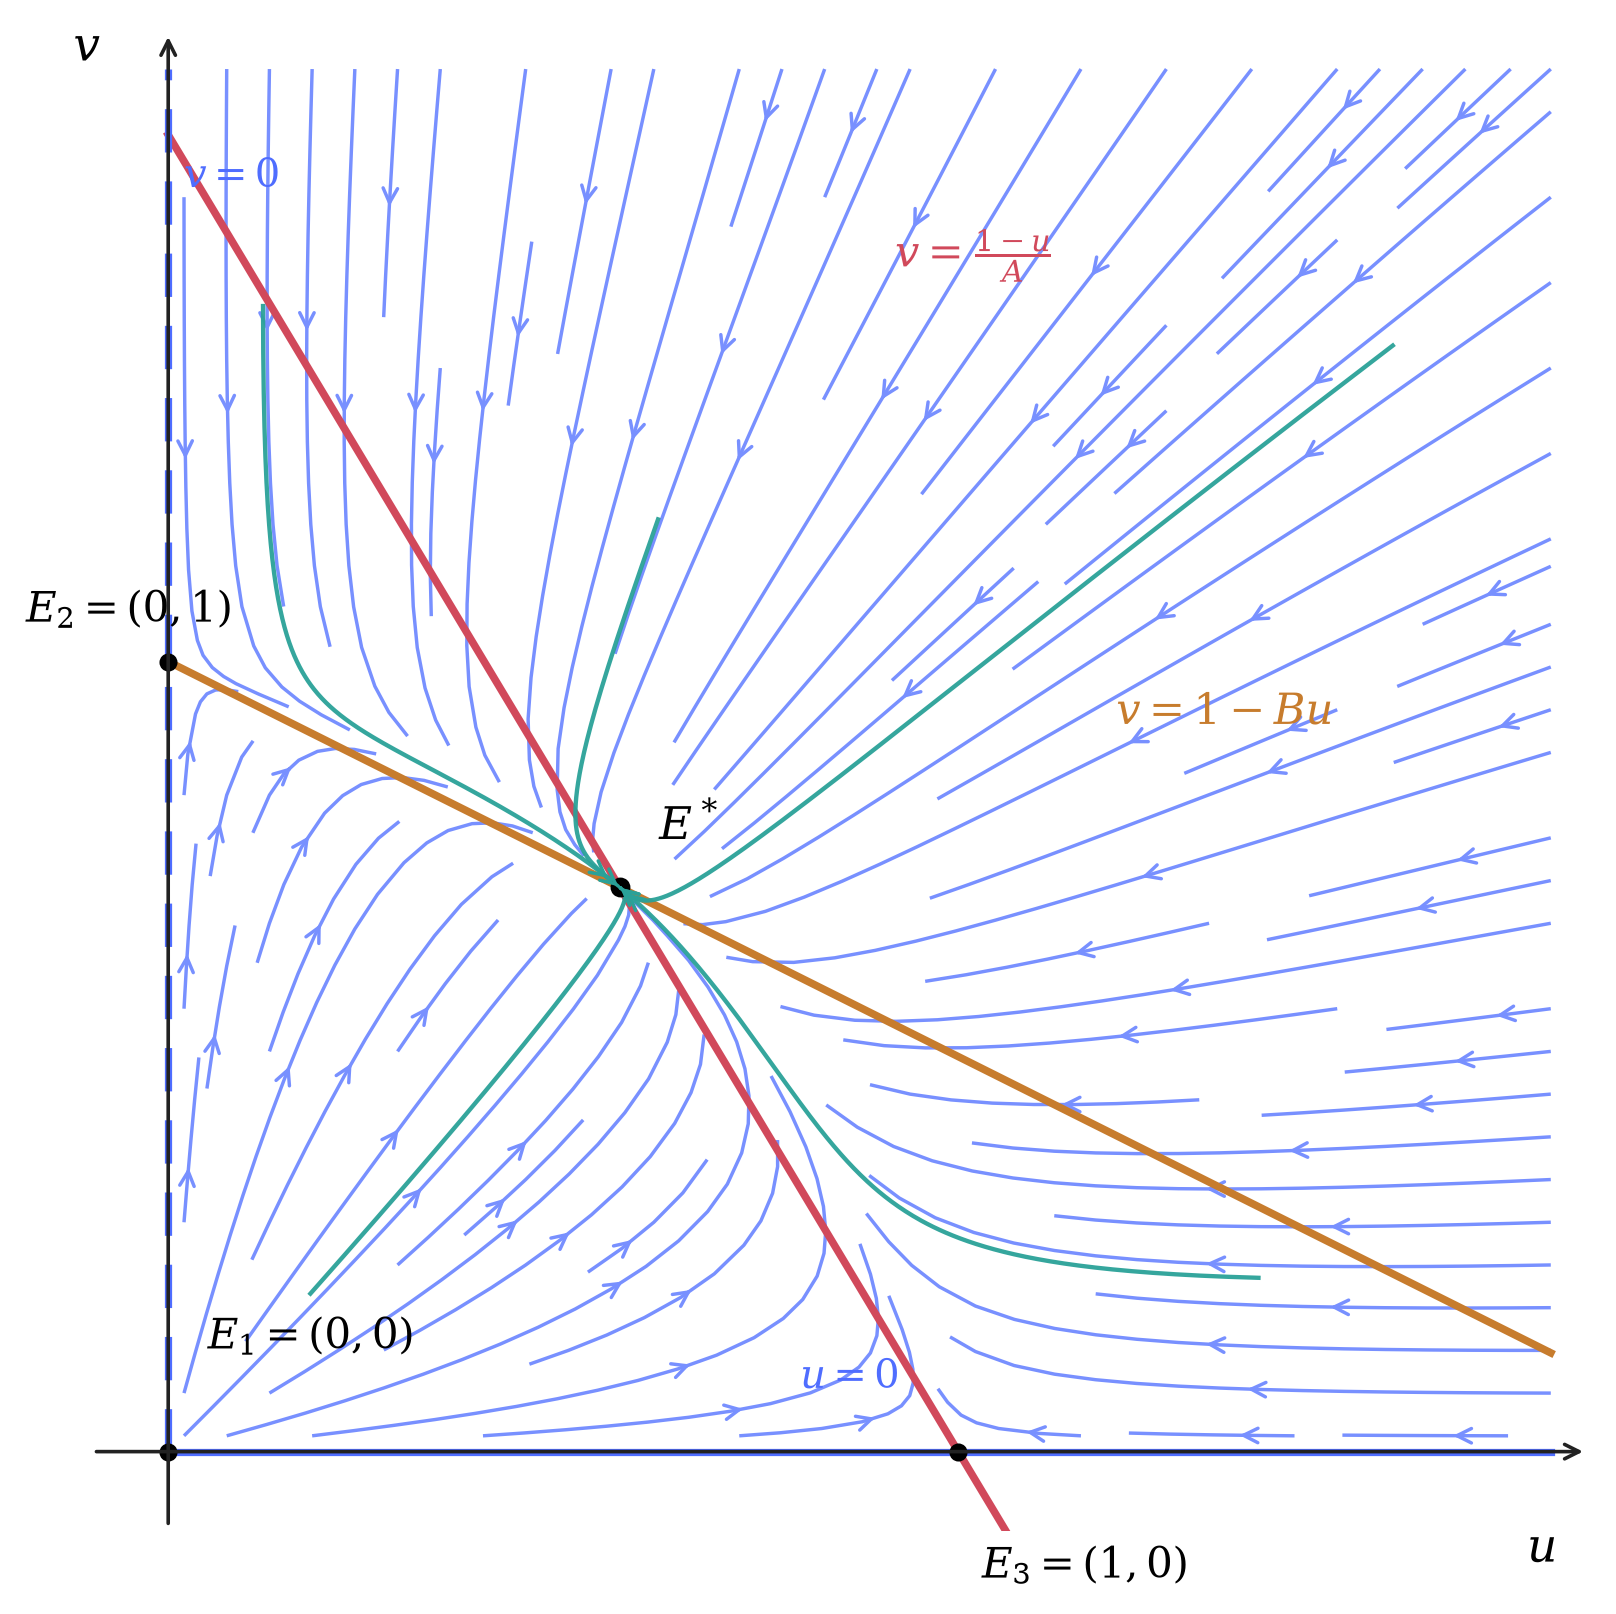
\includegraphics[width=0.92\linewidth]{fig_35_competencia_26Jun26.png}
\caption{Retrato de fase del sistema de competencia: ejes invariantes,
isoclinas nulas (recta de $u'=0$ con interceptos $(1,0)$ y $(0,1/A)$;
recta de $v'=0$ con interceptos $(1/B,0)$ y $(0,1)$), trayectorias
representativas y los cuatro equilibrios $E_1$, $E_2$, $E_3$ y $E^*$.}
\end{figure}

\subsection{29/06/2026}

Retomamos el sistema adimensionalizado de competencia entre dos especies:
\[
\dot u = u(1-u-\alpha v), \qquad
\dot v = \rho\,v(1-v-\beta u),
\]
con $\alpha,\beta,\rho>0$.

\subsubsection*{Isoclinas nulas y puntos de equilibrio}

Las isoclinas nulas son:
\begin{itemize}
    \item Para $\dot u=0$: $u=0$ \quad o \quad $1-u-\alpha v=0$.
    \item Para $\dot v=0$: $v=0$ \quad o \quad $1-v-\beta u=0$.
\end{itemize}

Combinando las condiciones $\dot u=0$ y $\dot v=0$ se obtienen cuatro puntos de equilibrio:
\begin{enumerate}
    \item $E_1=(0,0)$.
    \item $u=0$, $1-v-\beta u=0 \Rightarrow v=1$, luego $E_2=(0,1)$.
    \item $v=0$, $1-u-\alpha v=0 \Rightarrow u=1$, luego $E_3=(1,0)$.
    \item El equilibrio interior $E^*$ satisface simultáneamente
    \[
    u+\alpha v=1,\qquad \beta u+v=1,
    \]
    es decir, el sistema lineal
    \[
    \begin{pmatrix}1 & \alpha\\ \beta & 1\end{pmatrix}
    \begin{pmatrix}u\\v\end{pmatrix}
    =\begin{pmatrix}1\\1\end{pmatrix}.
    \]
    El determinante de la matriz de coeficientes es $1-\alpha\beta$. Si $\alpha\beta\neq 1$, la solución única es
    \[
    \begin{pmatrix}u^*\\v^*\end{pmatrix}
    =\frac{1}{1-\alpha\beta}
    \begin{pmatrix}1 & -\alpha\\-\beta & 1\end{pmatrix}
    \begin{pmatrix}1\\1\end{pmatrix}
    =\frac{1}{1-\alpha\beta}\begin{pmatrix}1-\alpha\\1-\beta\end{pmatrix},
    \]
    es decir,
    \[
    \boxed{E^*=\left(\frac{1-\alpha}{1-\alpha\beta},\;\frac{1-\beta}{1-\alpha\beta}\right).}
    \]
\end{enumerate}

\begin{observacion}{Positividad del equilibrio interior}{}
El equilibrio $E^*$ pertenece al primer cuadrante ($u^*,v^*>0$) exactamente en dos casos:
\begin{itemize}
    \item \textbf{Caso $0<\alpha,\beta<1$:} entonces $1-\alpha>0$, $1-\beta>0$ y $1-\alpha\beta>0$,
          por lo que $u^*=(+)/(+)>0$ y $v^*=(+)/(+)>0$.
    \item \textbf{Caso $\alpha,\beta>1$:} entonces $1-\alpha<0$, $1-\beta<0$ y $1-\alpha\beta<0$,
          por lo que $u^*=(-)/(-)>0$ y $v^*=(-)/(-)>0$.
\end{itemize}
En cualquier otro caso $E^*$ no es biológicamente viable.
\end{observacion}

\subsubsection*{Análisis de signos del campo}

El signo de cada componente del campo queda determinado por la posición relativa a las isoclinas:
\begin{itemize}
    \item $\dot u > 0$ si y solo si $u>0$ y $v < \dfrac{1-u}{\alpha}$,
          es decir, para puntos del primer cuadrante \emph{por debajo} de la recta $1-u-\alpha v=0$.
    \item $\dot u < 0$ para puntos del primer cuadrante \emph{por encima} de esa recta.
\end{itemize}
Un argumento análogo aplica para $\dot v$ respecto a la recta $1-v-\beta u=0$.

\begin{figure}[H]
\centering
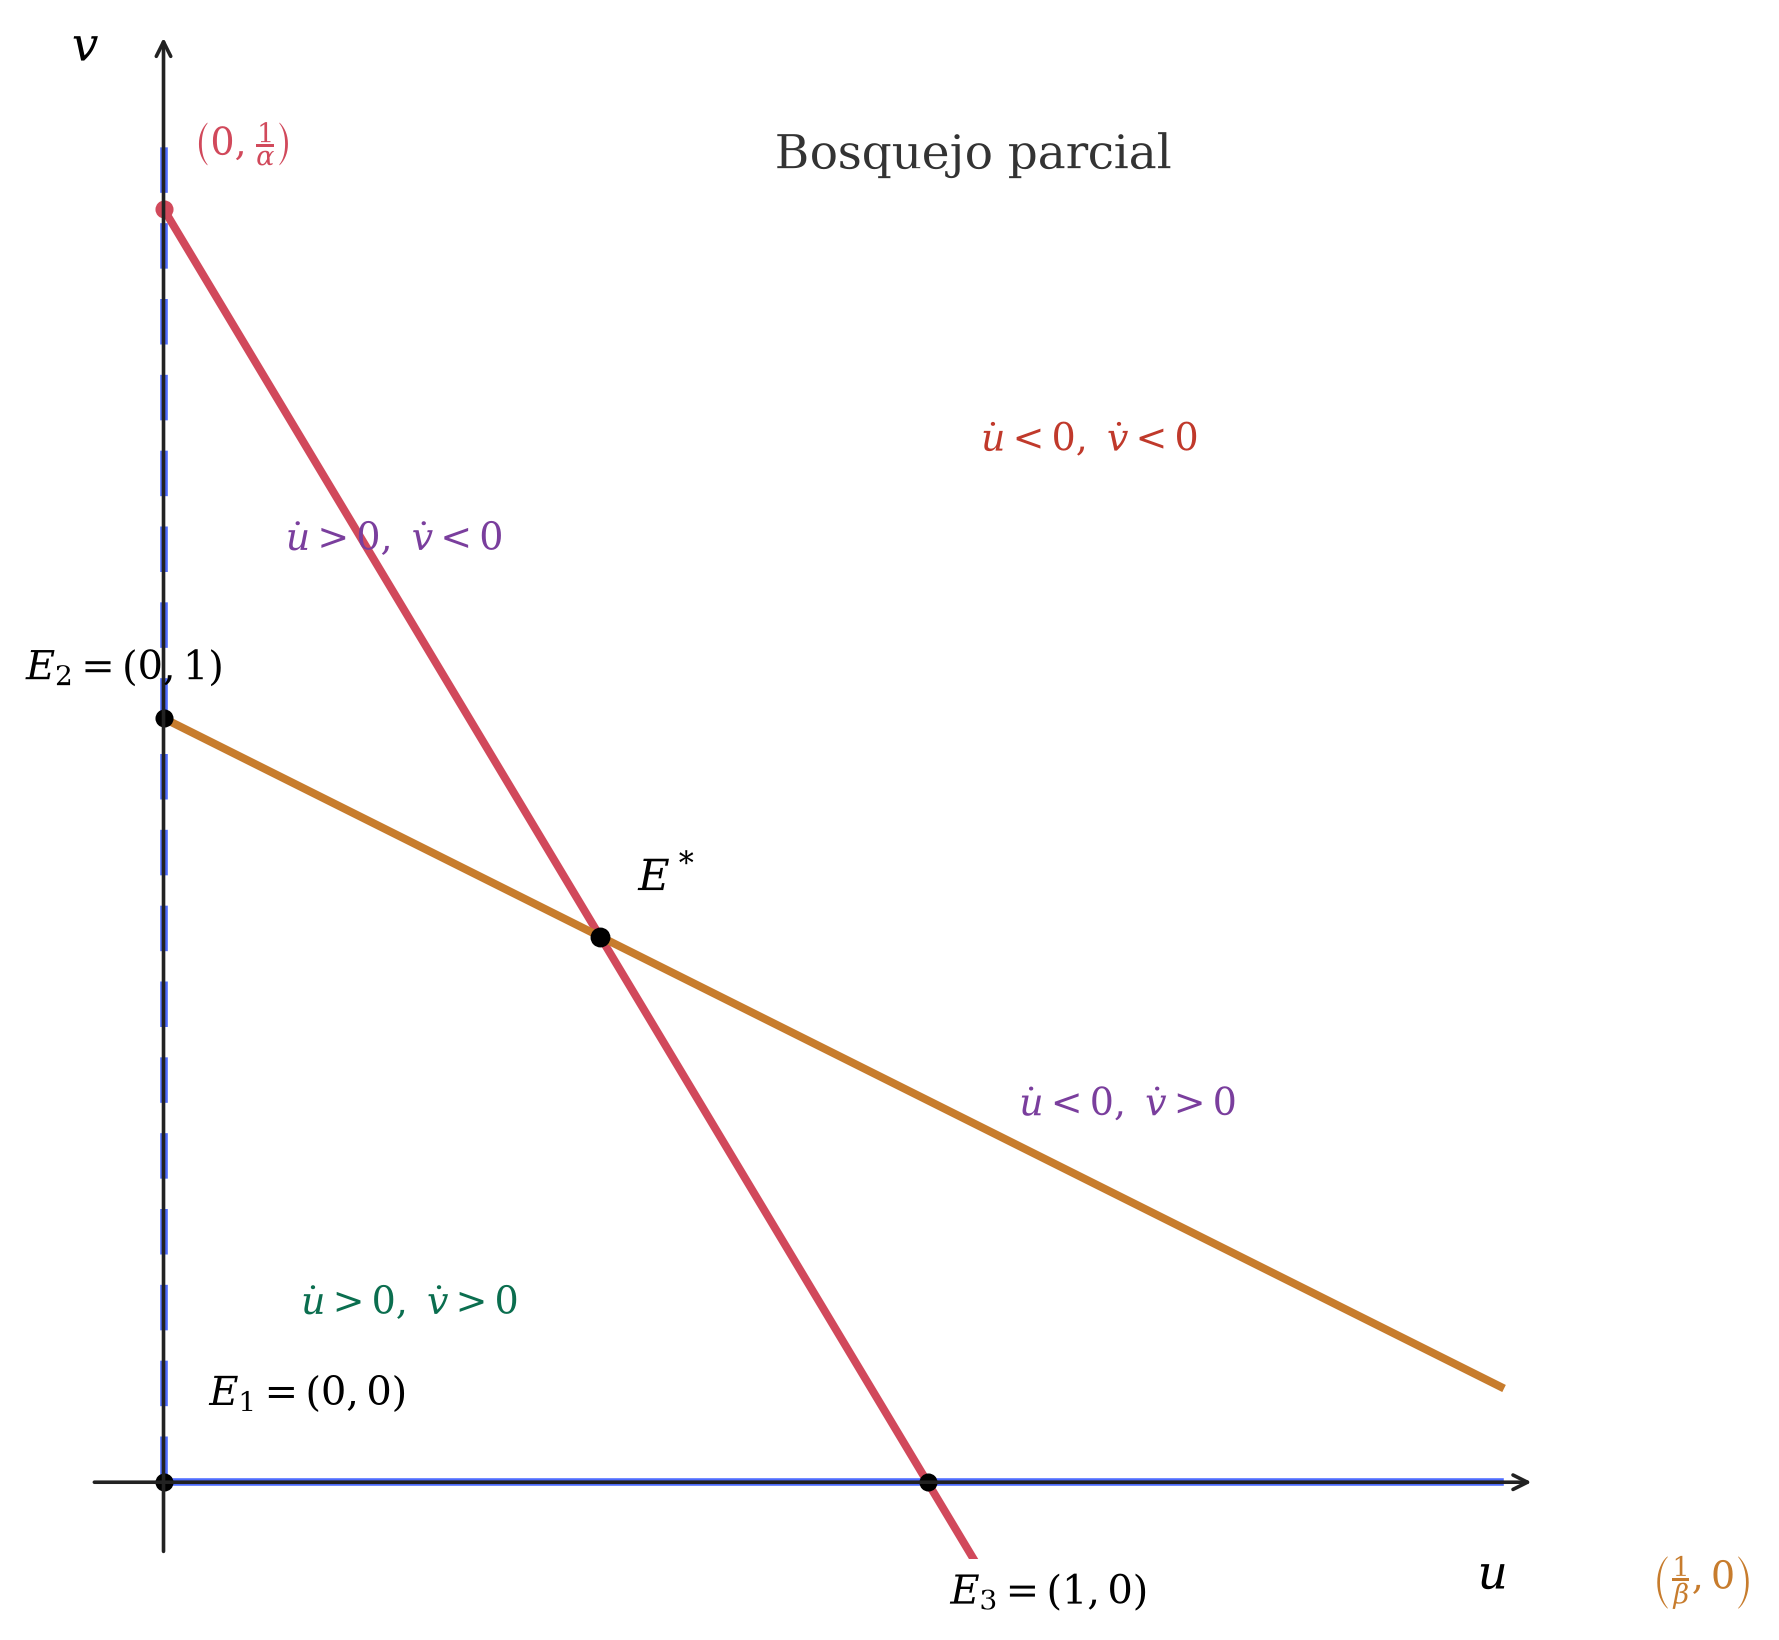
\includegraphics[width=0.92\textwidth]{fig_36_competencia_bosquejo_29Jun26.png}
\caption{Bosquejo del plano de fases a partir de las isoclinas nulas y los signos de $\dot u$ y $\dot v$.}
\end{figure}

\begin{figure}[H]
\centering
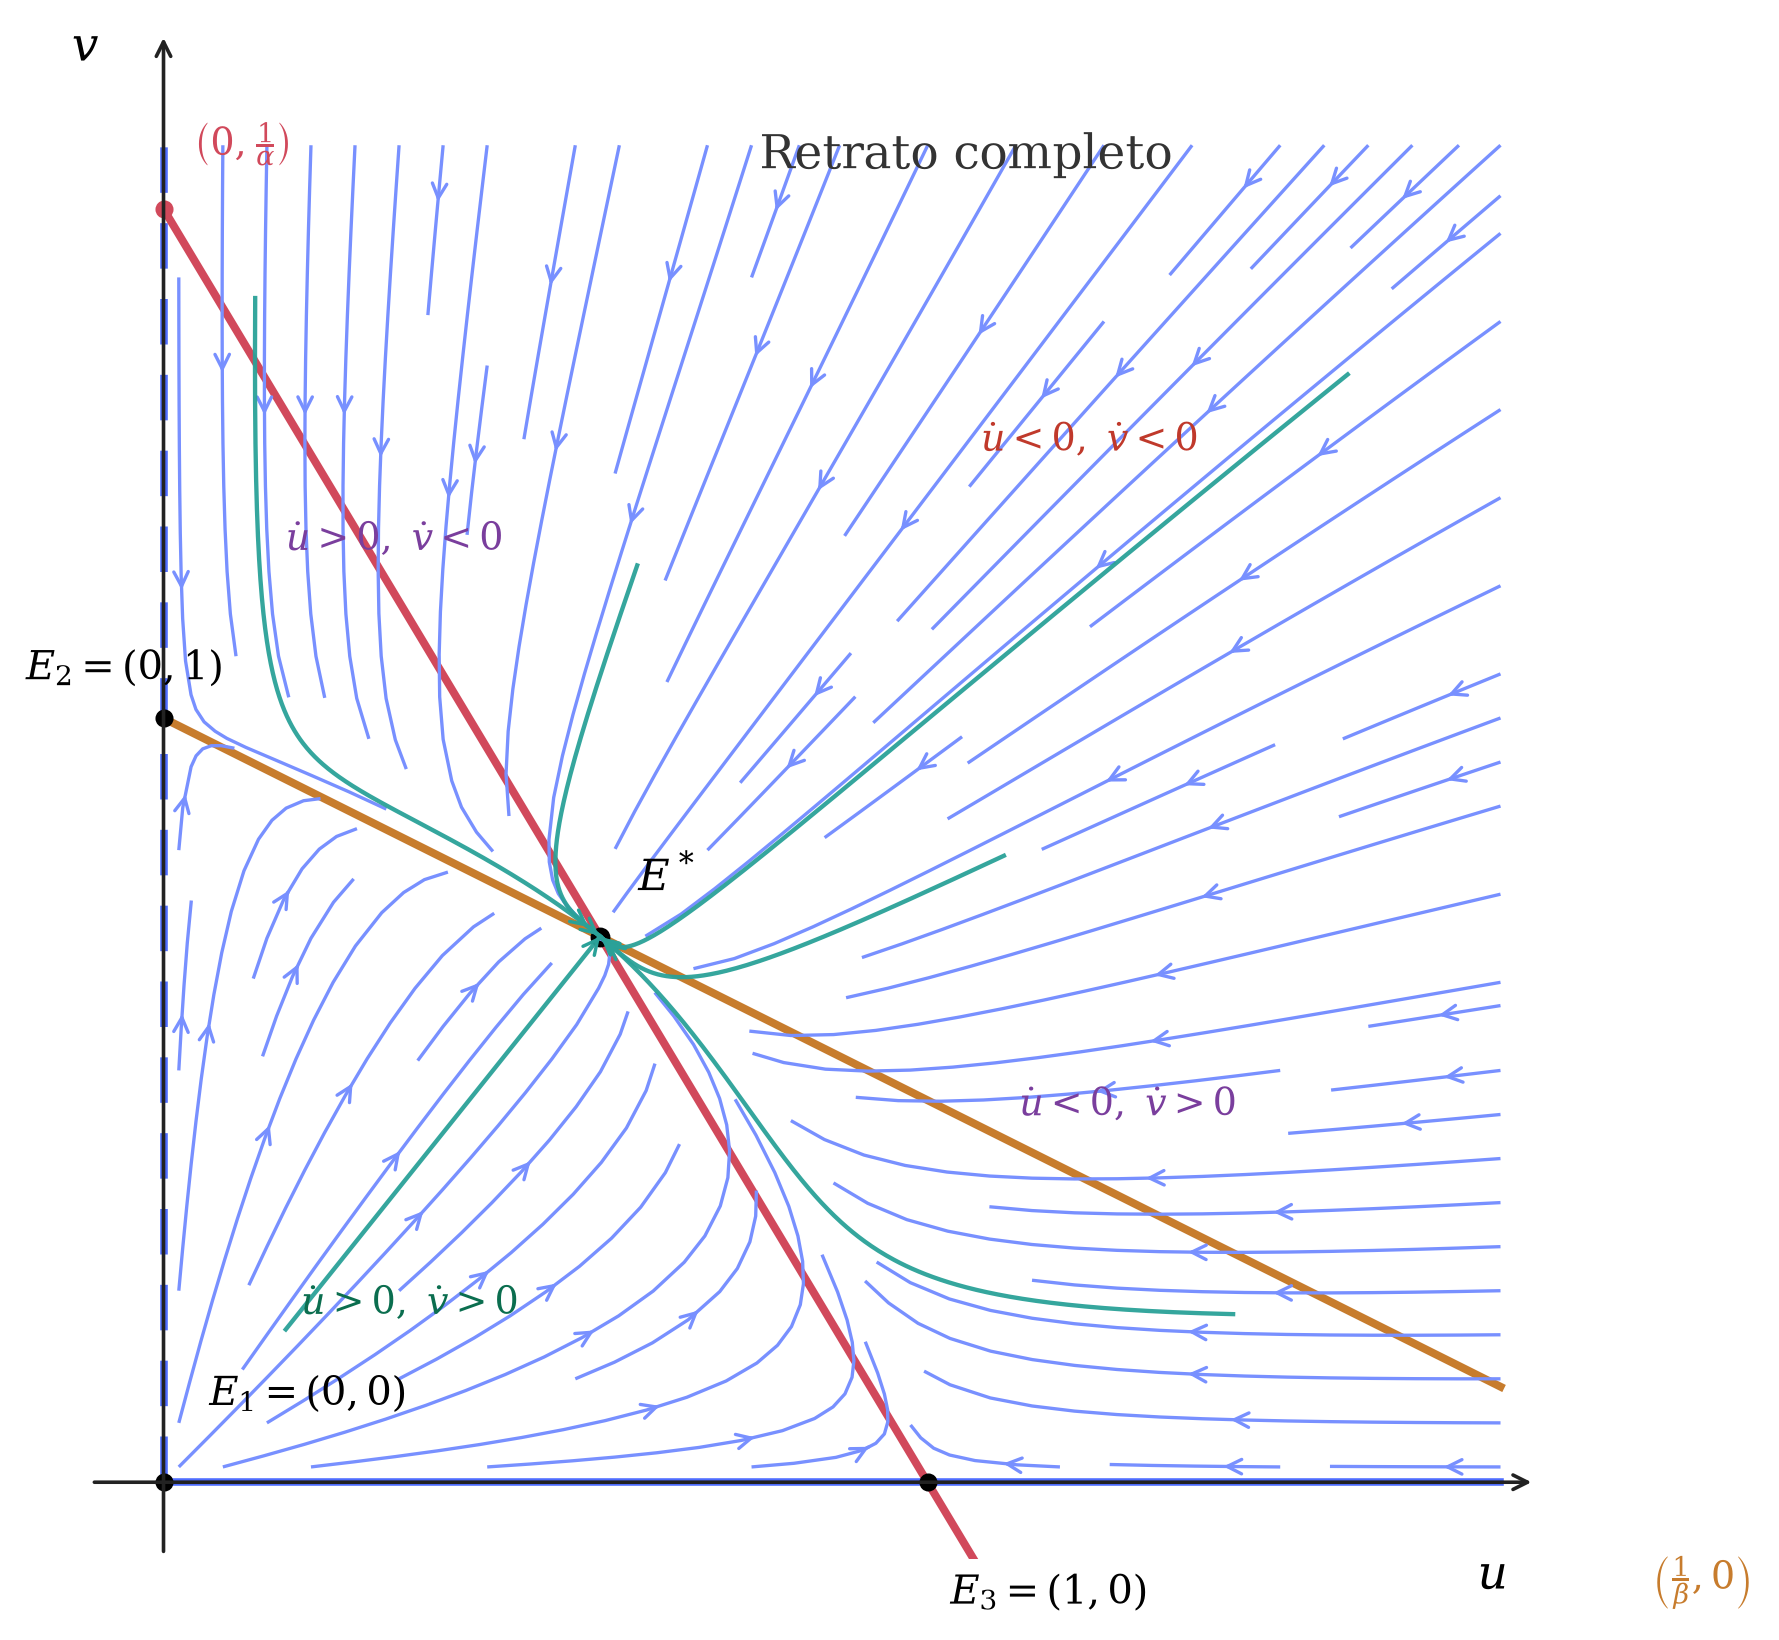
\includegraphics[width=0.92\textwidth]{fig_37_competencia_completa_29Jun26.png}
\caption{Retrato completo del plano de fases para el sistema de competencia, con dirección del campo y trayectorias representativas.}
\end{figure}

\subsubsection*{Estabilidad lineal de los equilibrios: caso $0<\alpha,\beta<1$}

El jacobiano del sistema es
\[
J(u,v)=
\begin{pmatrix}
1-2u-\alpha v & -\alpha u\\
-\rho\beta v & \rho(1-2v-\beta u)
\end{pmatrix}.
\]

\textbf{Equilibrio $E_1=(0,0)$:}
\[
J(E_1)=\begin{pmatrix}1 & 0\\ 0 & \rho\end{pmatrix}.
\]
Los valores propios $\lambda_1=1>0$ y $\lambda_2=\rho>0$ son positivos; $E_1$ es hiperbólico.
Por el teorema de Hartman--Grobman, $E_1$ es localmente una \textbf{fuente}.

\textbf{Equilibrio $E_2=(0,1)$:}
\[
J(E_2)=\begin{pmatrix}1-\alpha & 0\\ -\rho\beta & -\rho\end{pmatrix}.
\]
Al ser triangular, los valores propios son $\lambda_1=1-\alpha$ y $\lambda_2=-\rho<0$.
Como $0<\alpha<1$, se tiene $\lambda_1>0$: los valores propios tienen signos opuestos.
$E_2$ es hiperbólico y, por Hartman--Grobman, localmente un \textbf{punto silla}.

\textbf{Equilibrio $E_3=(1,0)$:}
\[
J(E_3)=\begin{pmatrix}-1 & -\alpha\\ 0 & \rho(1-\beta)\end{pmatrix}.
\]
Al ser triangular, los valores propios son $\lambda_1=-1<0$ y $\lambda_2=\rho(1-\beta)$.
Como $0<\beta<1$, se tiene $\lambda_2>0$: los valores propios tienen signos opuestos.
$E_3$ es hiperbólico y localmente un \textbf{punto silla}.

\subsubsection*{Estabilidad del equilibrio interior $E^*$}

\begin{observacion}{Traza y determinante en una matriz $2\times 2$}{}
Para cualquier matriz $A$ de $2\times 2$: la traza es la suma de los valores propios y el determinante es su producto. En particular:
\begin{itemize}
    \item $\det(A)>0$ implica que los valores propios tienen el mismo signo (o son complejos conjugados con parte real del mismo signo).
    \item $\det(A)<0$ implica que los valores propios tienen signos opuestos (punto silla).
    \item El signo de $\operatorname{Tr}(A)$ determina si la suma es positiva o negativa.
\end{itemize}
\end{observacion}

Como $(u^*,v^*)$ satisface las ecuaciones de isoclinas, se pueden simplificar las entradas del jacobiano:
\[
1-u^*-\alpha v^*=0 \;\Rightarrow\; 1-2u^*-\alpha v^* = -u^*,
\]
\[
1-v^*-\beta u^*=0 \;\Rightarrow\; 1-2v^*-\beta u^* = -v^*.
\]
El jacobiano evaluado en $E^*$ se reduce a la forma elegante:
\[
\boxed{J(E^*)=\begin{pmatrix}-u^* & -\alpha u^*\\ -\rho\beta v^* & -\rho v^*\end{pmatrix}.}
\]

\begin{observacion}{Traza de $J(E^*)$ en el caso $0<\alpha,\beta<1$}{}
Como $u^*,v^*>0$, la traza satisface
\[
\operatorname{Tr}(J(E^*))=-u^*-\rho v^*<0.
\]
Esto garantiza que al menos uno de los valores propios es negativo. La clasificación completa de $E^*$ depende del signo del determinante:
si $\det(J(E^*))>0$, ambos valores propios son negativos y $E^*$ es un \textbf{sumidero} (coexistencia estable);
si $\det(J(E^*))<0$, los valores propios tienen signos opuestos y $E^*$ es una \textbf{silla} (bistabilidad).
\end{observacion}

% Pendiente: análisis de imágenes 7 y 8.

% ============================================================
\section{Dinámica de dos poblaciones: modelo general}
\label{sec:modelo-general-dos-poblaciones}
% ============================================================

La versión anterior de Lotka-Volterra se puede enriquecer incorporando
capacidad de carga en la presa y una respuesta funcional más general $f(P)$:
\[
\frac{dP}{dt}=rP\!\left(1-\frac{P}{K}\right)-f(P)D,\qquad
\frac{dD}{dt}=-\gamma D+\delta f(P)D.
\]
El caso $f(P)=P$ recupera el sistema clásico. Esta formulación sirve como
puente entre el modelo básico y sus variantes ecológicas más realistas, como
la respuesta funcional de Holling tipo II: $f(P)=P/(1+hP)$, que satura
cuando la presa es abundante.

% ============================================================
\section{Ejercicios de cierre y correspondencias}
\label{sec:tarea-referencia}
% ============================================================

\subsection{EDOs: cinética química}

\begin{enumerate}
\item Sistema $A'=-kA$, $B'=kA$, $A(0)=A_0$, $B(0)=0$.
      Solución completa en la Sección~\ref{sec:cinetica} (reacción $A\to B$).
\item Sistema $A'=-2kA^2$, $B'=kA^2$, $A(0)=A_0$, $B(0)=0$.
      Solución completa en la Sección~\ref{sec:cinetica} (ley de acción de masas).
\end{enumerate}

\subsection{Estabilidad: modelo logístico}

Los incisos (a)--(e) se desarrollan en la Sección~\ref{sec:modelo-logistico}:
equilibrios, análisis geométrico, linealización, concordancia y solución analítica.

\subsection{Adimensionalización}

\begin{itemize}
    \item Problemas 1--3 (logístico, cosecha, Allee): Sección~\ref{sec:adimensionalizacion}.
    \item Problema 4 (caída libre con resistencia): Sección~\ref{sec:adimensionalizacion}.
    \item Problema 5 (oscilador amortiguado): Sección~\ref{sec:adimensionalizacion}.
    \item Problema 8 (Lotka-Volterra): Sección~\ref{sec:lotka-volterra}.
    \item Problema 10 (péndulo): Sección~\ref{sec:adimensionalizacion}.
    \item Problema 11 (circuito RC): Sección~\ref{sec:ecuaciones-lineales-primer-orden}.
\end{itemize}

\subsection{Bifurcaciones (al menos 5 de 10)}

La Sección~\ref{sec:bifurcaciones-unidim} reúne los tipos silla-nodo,
transcrítica, pitchfork supercrítica y pitchfork subcrítica con ejemplos
canónicos que corresponden directamente a los ejercicios (a), (b), (c), (d),
(f), (g), (h) del listado.

\subsection{Sistemas lineales y Hartman-Grobman}

El ejemplo trabajado del sistema $x_1'=-x_1+x_1^2$, $x_2'=-2x_2+x_1^2$
en la Sección~\ref{sec:hartman-grobman} cubre el análisis completo:
cálculo del jacobiano, valores y vectores propios, clasificación de los
equilibrios $X_0$ y $X_1$ y aplicación del teorema.

\end{document}
